% Generated by scripts/build_readers.py; change the reviewed sources and rebuild.
\def\EditionMode{1}
\def\EditionLabel{Corrected reader with apparatus}
\def\EditionStatus{WORKING EDITION: 27 of 706 source pages reviewed and included}
\documentclass[10pt,oneside]{book}
\usepackage{fontspec}
\setmainfont{Latin Modern Roman}
\setsansfont{Latin Modern Sans}
\usepackage{amsmath,amssymb,mathtools}
\usepackage{unicode-math}
\setmathfont{Latin Modern Math}
\usepackage{xcolor,tikz-cd,lua-ul,marginnote,pdflscape}
\usetikzlibrary{arrows.meta,decorations.pathmorphing,calc,shapes.geometric}
\tikzcdset{ampersand replacement=\&}
\tikzcdset{every label/.append style={text=black}}
\usepackage[a4paper,left=18mm,right=45mm,top=18mm,bottom=22mm,marginparwidth=28mm,marginparsep=7mm]{geometry}
\usepackage[unicode,colorlinks=true,urlcolor=black,linkcolor=black]{hyperref}
\usepackage{bookmark}
\setlength{\parindent}{0pt}
\setlength{\parskip}{4pt plus 1pt minus 1pt}
\setlength{\emergencystretch}{1.5em}
\raggedbottom
\definecolor{PSHand}{RGB}{25,58,132}
\definecolor{PSDelete}{RGB}{146,37,37}
\definecolor{PSTypedOld}{RGB}{95,95,95}
\ifnum\EditionMode=2\colorlet{blue}{black}\else\colorlet{blue}{PSHand}\fi
\RenewDocumentCommand{\textcircled}{m}{\tikz[baseline=(PSCircle.base)]\node[draw,circle,inner sep=.5pt,line width=.4pt](PSCircle){#1};}
\newif\ifPSInApparatus
\newcounter{psnote}
\newcounter{psvariant}
\newcounter{pslinkmark}
\newif\ifPSInLink
\newsavebox{\PSNoteBox}
\newdimen\PSNoteLimit
{\footnotesize\global\PSNoteLimit=3\baselineskip}
\newcommand{\CurrentScanURL}{}
\newcommand{\CurrentKey}{}
\newcommand{\CurrentScan}{}
\newcommand{\pssource}[3]{\psflushmargins\clearpage\gdef\CurrentKey{#1}\gdef\CurrentScan{#2}\gdef\CurrentScanURL{#3}\setcounter{psvariant}{0}\typeout{PS-SOURCE: #1}}
\newcommand{\pslinkmarker}[2]{\stepcounter{pslinkmark}\latelua{texio.write_nl('log','PS-LINK-SHIP|#1|\CurrentKey|\arabic{pslinkmark}|#2')}}
\newcommand{\pslink}[2]{\ifPSInLink\pslinkmarker{#1}{nested}#2\else\begingroup\PSInLinktrue\href{\CurrentScanURL}{\pslinkmarker{#1}{outer}#2}\endgroup\fi}
\newcommand{\scanpage}[1]{\ifnum\EditionMode=2\marginnote{\scriptsize\sffamily\pslink{scanpage}{scan #1}}\else\par\noindent{\small\sffamily\pslink{scanpage}{[scan #1]}}\par\medskip\fi}
\newcommand{\mspage}[1]{\ifnum\EditionMode=2\marginnote{\scriptsize\sffamily p.\,#1}\else{\small\sffamily[p.\,#1]}\fi}
\newcommand{\hand}[1]{{\ifnum\EditionMode=2\color{black}\else\color{PSHand}\fi #1}}
\let\over\relax
\NewDocumentCommand{\over}{O{} m m}{{\textcolor{PSTypedOld}{#2}\ensuremath{^{\!\nearrow}}\if\relax\detokenize{#1}\relax\hand{#3}\else #3\fi}}
\NewDocumentCommand{\inserted}{O{} m}{{\if\relax\detokenize{#1}\relax\hand{\ensuremath{\langle}#2\ensuremath{\rangle}}\else\ensuremath{\langle}#2\ensuremath{\rangle}\fi}}
\newcommand{\deleted}[1]{{\color{PSDelete}\ifmmode\text{[del.: }#1\text{]}\else[\textsf{del.:} #1]\fi}}
\newcommand{\xout}[1]{{\color{PSTypedOld}\ifmmode\text{[x: }#1\text{]}\else[\textsf{x:} #1]\fi}}
\let\PSMathUnderline\underline
\RenewDocumentCommand{\underline}{+m}{\ifmmode\PSMathUnderline{#1}\else\underLine{#1}\fi}
\NewDocumentCommand{\uline}{+m}{\underline{#1}}
\NewDocumentCommand{\uuline}{+m}{\ifmmode\PSMathUnderline{\PSMathUnderline{#1}}\else\underLine{\underLine{#1}}\fi}
\newunderlinetype\PSWaveLine{\leaders\hbox{\lower.7ex\hbox{\tikz[x=1pt,y=1pt,baseline=0pt]{\draw[line width=.3pt] (0,0) .. controls (1,1) and (2,1) .. (3,0) .. controls (4,-1) and (5,-1) .. (6,0);}}}}
\NewDocumentCommand{\uwave}{+m}{{\PSWaveLine #1}}
\newcommand{\unsure}[1]{\pslink{unsure}{[#1\ifmmode\,?\else\,?\fi]}}
\newcommand{\illegible}[1]{\ifmmode\text{\pslink{illegible}{[illeg.\ #1]}}\else\pslink{illegible}{[illeg.\ #1]}\fi}
\NewDocumentCommand{\diagram}{+m}{\ifmmode\vcenter{\hbox{#1}}\else\par\medskip{\centering #1\par}\medskip\psflushmargins\fi}
\newenvironment{diagramblock}{\par\begin{center}}{\end{center}\par}
\newcommand{\PSMathNotes}{}
\makeatletter
\NewDocumentCommand{\psplacednote}{m +m}{%
      \sbox{\PSNoteBox}{\parbox{\marginparwidth}{\footnotesize\raggedright\hand{\textsf{m#1.} #2}}}%
      \ifdim\dimexpr\ht\PSNoteBox+\dp\PSNoteBox\relax<\PSNoteLimit
        \leavevmode\marginpar{\usebox{\PSNoteBox}}%
      \else
        \par\nobreak\smallskip\hrule\nobreak\smallskip
        {\footnotesize\textsf{Marginal note m#1.}\quad\hand{#2}\par}
        \nobreak\smallskip\hrule\smallskip
      \fi}
\newcommand{\psflushmargins}{\ifmmode\else\ifinner\else\ifx\PSMathNotes\@empty\else\let\PSTempNotes\PSMathNotes\global\let\PSMathNotes\@empty\PSTempNotes\fi\fi\fi}
\NewDocumentCommand{\margin}{+m}{%
  \ifPSInApparatus\ifmmode\hand{\text{[marg.: }#1\text{]}}\else\hand{\textsf{[marg.: }#1\textsf{]}}\fi
  \else\stepcounter{psnote}%
    \ifmmode
      \text{\textsuperscript{m\arabic{psnote}}}%
      \begingroup\edef\PSQueue{\endgroup\noexpand\g@addto@macro\noexpand\PSMathNotes{\noexpand\psplacednote{\arabic{psnote}}{\unexpanded{$#1$}}}}\PSQueue
    \else
      \textsuperscript{m\arabic{psnote}}\psplacednote{\arabic{psnote}}{#1}%
    \fi
  \fi}
\AtBeginDocument{\everymath\expandafter{\the\everymath\aftergroup\psflushmargins}\everydisplay\expandafter{\the\everydisplay\aftergroup\psflushmargins}}
\makeatother
\newcommand{\psnumber}[2]{\expandafter\gdef\csname psnum@#1\endcsname{#2}}
\NewDocumentCommand{\var}{+m +m m m}{\ifnum\EditionMode=0 #1\else\ifnum\EditionMode=1\ifmmode\text{\textsuperscript{\tiny\csname psnum@#4\endcsname}}\else\textsuperscript{\tiny\csname psnum@#4\endcsname}\fi\fi #2\fi}
\newcommand{\psapparatusstart}{\par\bigskip\hrule\smallskip\PSInApparatustrue\begingroup\footnotesize\textsf{Apparatus for scan \CurrentScan}\par}
\newcommand{\psapparatusend}{\par\endgroup\PSInApparatusfalse}
\NewDocumentCommand{\psentry}{m m m +m +m m}{\par\noindent\textbf{#2. #3.}\quad\textit{Typescript:} #4\quad\textit{Corrected:} \if\relax\detokenize{#5}\relax\textnormal{[omitted]}\else #5\fi\quad #6\par}
\newcommand{\psfrontmatter}{%
\hypersetup{pageanchor=false}\begin{titlepage}\raggedright
{\Large Alexander Grothendieck\par}\vspace{12mm}
{\Huge Pursuing Stacks\par}\medskip{\LARGE 1983\par}\vspace{12mm}
{\Large\EditionLabel\par}\vspace{8mm}
{\large\EditionStatus\par}\vfill
Université de Montpellier, Grothendieck archive, cotes 134-2--134-8.\par
Including the 26 source pages of R. Brown's translation at cote 134-2, sites 115--143.\par
\end{titlepage}\hypersetup{pageanchor=true}
\chapter*{Editorial statement}
AI-transcribed by Claude Opus 5.5 (Anthropic, effort high); checked against the scans, and this edition built, by GPT-6 Astra (OpenAI, ChatGPT Pro mode); prompts and records by Claude (Anthropic).

The witness consulted and not reproduced is the LaTeX edition of Mateo Carmona with the collaboration of Ulrik Buchholtz (arXiv 2111.01000 v2, 2021), extended from the 2015 edition by ``the scrivener'', CC0 1.0.

The translation in the appendix is R. Brown's, prepared with assistance from L. Breen and J-L. Loday, as his note says; the rights in it belong to its translator or his heirs.

The rights in the original work belong to its author or the author's representatives or heirs. Where we hold rights, in the AI-produced transcription, translation, corrections and typesetting, they are dedicated to the public domain under CC0 1.0. This edition is published for educational, non-profit purposes, and we claim no rights we do not hold. If you hold rights in this work and object to its publication here, please open a GitHub issue and we will take it down.

\section*{How to read this form}
\ifnum\EditionMode=0
The diplomatic form preserves typed and handwritten wording, cancellations, insertions, overwritten readings, underlining, doubts, and original page numbers. Blue marks handwriting; red labels handwritten cancellations; gray labels typewriter cancellations and underlying overwritten text. Angle brackets mark insertions; a superscript arrow separates an overwritten reading from its replacement. Typed insertions and typed overwriting remain plain. The disposition of long marginal notes is identified explicitly.
\else
The corrected text applies the author's insertions, replacements, cancellations, and recorded transpositions. It retains his English and notation, including consistent forms such as ``standart'', ``developped'', ``it's'' for ``its'', and ``A la''. An isolated slip is corrected only when specifically recorded and justified. Mathematical anomalies are preserved and discussed in the guide.
\ifnum\EditionMode=1
Blue continues to identify handwriting. A numbered call identifies each maximal editorial operation, with its full diplomatic and corrected readings and reason in the apparatus following the source page. Internal layers of a wholly replaced or deleted passage are preserved within that entry rather than duplicated as separate entries. These entries are generated from the same variants that govern the running text.
\else
This reading form omits the apparatus, cancelled material, superseded readings, insertion brackets, and color distinctions. It retains the resulting text, marginal notes, underlining, and unresolved doubts. Scan and source-page references appear in the margin.
\fi\fi

Every scan mark and remaining doubt links to its source page in the archive viewer. Doubts are editorial reading marks, not emendations. The source-page breaks identify the archival sequence; a source page may occupy more than one printed page. A partial working edition is explicitly labelled and contains only reviewed source pages.
\clearpage}

\begin{document}
\psfrontmatter
\pssource{ps_134-2_001}{134-2/1}{https://grothendieck.umontpellier.fr/web/viewer.html?file=../134-2.pdf\#page=2}
%% BEGIN SOURCE ps_134-2_001
% Pursuing Stacks (cotes 134-2 to 134-8): archive cote 134-2, site page 1 (PDF page 2).
% front matter. Draft compared: none.
% AI-transcribed by Claude Opus 5.5 (claude-opus-5-5, adaptive thinking, effort high), Message Batches API, batch ps1 (msgbatch_01Rv5hCaNTtUt4JHx1yqoHPL), 2026-11-12; reviewed against both supplied scan halves; see CHECK_DECISIONS.tsv.
\scanpage{134-2/1}
\hand{The \unsure{Modelizing|Modelising} Story}\par

\margin{\unsure{$\checkmark$}}\par

% NOTE: the rest of the page is blank apart from stains and a few faint pencil marks

\mspage{\hand{1}}

%% END SOURCE ps_134-2_001
\pssource{ps_134-2_002}{134-2/2}{https://grothendieck.umontpellier.fr/web/viewer.html?file=../134-2.pdf\#page=3}
\psnumber{ps_134-2_002-v0001}{1}
\psnumber{ps_134-2_002-v0002}{2}
\psnumber{ps_134-2_002-v0003}{3}
\psnumber{ps_134-2_002-v0004}{4}
\psnumber{ps_134-2_002-v0005}{5}
\psnumber{ps_134-2_002-v0006}{6}
\psnumber{ps_134-2_002-v0007}{7}
\psnumber{ps_134-2_002-v0008}{8}
\psnumber{ps_134-2_002-v0009}{9}
\psnumber{ps_134-2_002-v0010}{10}
\psnumber{ps_134-2_002-v0011}{11}
\psnumber{ps_134-2_002-v0012}{12}
\psnumber{ps_134-2_002-v0013}{13}
\psnumber{ps_134-2_002-v0014}{14}
%% BEGIN SOURCE ps_134-2_002
% Pursuing Stacks (cotes 134-2 to 134-8): archive cote 134-2, site page 2 (PDF page 3).
% front matter. Draft compared: none.
% AI-transcribed by Claude Opus 5.5 (claude-opus-5-5, adaptive thinking, effort high), Message Batches API, batch ps1 (msgbatch_01Rv5hCaNTtUt4JHx1yqoHPL), 2026-11-12; reviewed against both supplied scan halves; see CHECK_DECISIONS.tsv.
\scanpage{134-2/2}
THE MODELIZING STORY\par

(\var{\over{\unsure{h}}{H}}{\hand{H}}{writing over}{ps_134-2_002-v0001}istoire de \var{\over{\unsure{m}}{M}}{\hand{M}}{writing over}{ps_134-2_002-v0002}odèles)\par

\margin{\unsure{XI} Modelization (II)}\par

I \quad Take-off\par

II \quad \uline{Test categories} \var{\deleted{and test functors}}{}{deletion}{ps_134-2_002-v0003}\par

III \uline{Homotopy structures} \var{\deleted{and contractibility structures}}{}{deletion}{ps_134-2_002-v0004}\par

IV \quad \uline{Asphericity structures} \var{\deleted{and canonical modelizers}}{}{deletion}{ps_134-2_002-v0005}\par

\var{\inserted{Abelianization \unsure{\deleted{of homotopy types}} \unsure{I}}}{\hand{Abelianization \unsure{} \unsure{I}}}{insertion}{ps_134-2_002-v0006}\par
V \var{\deleted{Homology and cohomology (abelianization of homotopy types)}}{}{deletion}{ps_134-2_002-v0007}\par
\hand{\unsure{\var{\deleted{VII}}{}{deletion}{ps_134-2_002-v0008}}} \var{\inserted{Schematization \unsure{\deleted{of homotopy types}}}}{\hand{Schematization \unsure{}}}{insertion}{ps_134-2_002-v0009}\par

\var{\over{VI}{VIII}}{\hand{VIII}}{writing over}{ps_134-2_002-v0010} \uline{Homotopy} properties of (Cat) and A\^{} (closed model structures)\par

\hand{IX} \var{\deleted{VII}}{}{deletion}{ps_134-2_002-v0011} D\var{\over{\unsure{erivators|eriuators}}{erivators}}{\hand{erivators}}{writing over}{ps_134-2_002-v0012}\par

\hand{X} \var{\deleted{VIII}}{}{deletion}{ps_134-2_002-v0013} Back to topoi\par

\diagram{
\begin{tikzcd}
\hand{I} \& \hand{II} \arrow[color=blue, r, Rightarrow] \& \hand{III} \arrow[color=blue, r, Rightarrow] \& \hand{IV} \arrow[color=blue, d, Rightarrow] \& \hand{V\ \var{\deleted{VI}}{}{deletion}{ps_134-2_002-v0014}} \arrow[color=blue, dl, Rightarrow] \arrow[color=blue, d, Rightarrow] \arrow[color=blue, dr, Rightarrow] \& \\
 \& \& \& \hand{VIII} \arrow[color=blue, d, Rightarrow] \& \hand{VII} \& \hand{VI} \\
 \& \& \& \hand{IX} \& \&
\end{tikzcd}
}\par

\mspage{\hand{2}}

%% END SOURCE ps_134-2_002
\ifnum\EditionMode=1
\psapparatusstart
\psentry{ps_134-2_002-v0001}{1}{writing over}{\over{\unsure{h}}{H}}{\hand{H}}{The superposed handwritten reading replaces the underlying reading.}
\psentry{ps_134-2_002-v0002}{2}{writing over}{\over{\unsure{m}}{M}}{\hand{M}}{The superposed handwritten reading replaces the underlying reading.}
\psentry{ps_134-2_002-v0003}{3}{deletion}{\deleted{and test functors}}{}{The author cancels this material by hand; it leaves the corrected running text.}
\psentry{ps_134-2_002-v0004}{4}{deletion}{\deleted{and contractibility structures}}{}{The author cancels this material by hand; it leaves the corrected running text.}
\psentry{ps_134-2_002-v0005}{5}{deletion}{\deleted{and canonical modelizers}}{}{The author cancels this material by hand; it leaves the corrected running text.}
\psentry{ps_134-2_002-v0006}{6}{insertion}{\inserted{Abelianization \unsure{\deleted{of homotopy types}} \unsure{I}}}{\hand{Abelianization \unsure{} \unsure{I}}}{The handwritten insertion is incorporated at its indicated position; insertion brackets leave the running text.}
\psentry{ps_134-2_002-v0007}{7}{deletion}{\deleted{Homology and cohomology (abelianization of homotopy types)}}{}{The author cancels this material by hand; it leaves the corrected running text.}
\psentry{ps_134-2_002-v0008}{8}{deletion}{\deleted{VII}}{}{The author cancels this material by hand; it leaves the corrected running text.}
\psentry{ps_134-2_002-v0009}{9}{insertion}{\inserted{Schematization \unsure{\deleted{of homotopy types}}}}{\hand{Schematization \unsure{}}}{The handwritten insertion is incorporated at its indicated position; insertion brackets leave the running text.}
\psentry{ps_134-2_002-v0010}{10}{writing over}{\over{VI}{VIII}}{\hand{VIII}}{The superposed handwritten reading replaces the underlying reading.}
\psentry{ps_134-2_002-v0011}{11}{deletion}{\deleted{VII}}{}{The author cancels this material by hand; it leaves the corrected running text.}
\psentry{ps_134-2_002-v0012}{12}{writing over}{\over{\unsure{erivators|eriuators}}{erivators}}{\hand{erivators}}{The superposed handwritten reading replaces the underlying reading.}
\psentry{ps_134-2_002-v0013}{13}{deletion}{\deleted{VIII}}{}{The author cancels this material by hand; it leaves the corrected running text.}
\psentry{ps_134-2_002-v0014}{14}{deletion}{$\deleted{VI}$}{}{The author cancels this material by hand; it leaves the corrected running text.}
\psapparatusend
\fi
\pssource{ps_134-2_003}{134-2/3}{https://grothendieck.umontpellier.fr/web/viewer.html?file=../134-2.pdf\#page=4}
\psnumber{ps_134-2_003-v0001}{1}
\psnumber{ps_134-2_003-v0002}{2}
\psnumber{ps_134-2_003-v0003}{3}
\psnumber{ps_134-2_003-v0004}{4}
\psnumber{ps_134-2_003-v0005}{5}
\psnumber{ps_134-2_003-v0006}{6}
%% BEGIN SOURCE ps_134-2_003
% Pursuing Stacks (cotes 134-2 to 134-8): archive cote 134-2, site page 3 (PDF page 4).
% provisional contents. Draft compared: none.
% AI-transcribed by Claude Opus 5.5 (claude-opus-5-5, adaptive thinking, effort high), Message Batches API, batch ps1 (msgbatch_01Rv5hCaNTtUt4JHx1yqoHPL), 2026-11-12; reviewed against both supplied scan halves; see CHECK_DECISIONS.tsv.
\scanpage{134-2/3}
\mspage{i}

\margin{\uline{NB} Les chiffres souli-gnés \uline{5}, \uline{7}, \uline{13}, \uline{App.3}, \uline{App.6}, \uline{App 11}, \uline{App 12} etc sont à imprimer en caractères \unsure{gras}}\par

TABLE OF CONTENTS of The Modilizing Story (1) .\par

I \uline{Take-off} ( A letter to ... )\par

1. The importance of innocence.\par
2. A short look into purgatory.\par
3. ``Fundamental $\infty$-groupoids'' as objects of a ``model category'' ?\par
4. A bit of ordering in the mess of ``higher order structures''\hand{.}\par
\uline{5}. Jumping over the abyss !\par
6. The topological model; hemispheres building up the (tentative)\par
``universal $\infty$-- (co)groupoid''.\par
7. Gluing hemispheres: the ``standard'' amalgamations.\par
8. Description of the universal \uline{primitive} structure.\par
\uline{9}. The main inductive step: just add coherence arrows ! And the\par
abridged story of an (unescapable and irrelevant) ambiguity ...\par
10. Cutting down redundancies - or: ``l'embarras du choix''\hand{.}\par
\unsure{\hand{\textasciicircum}}11. Back to the topological model. The canonical functor from\par
spaces to `` $\infty$- groupoids'' .\par
12. About replacing spaces by objects of a ``model category''.\par
\uline{13}. An urgent reflection on proper names: ``stacks'' and ``coherators''\hand{.}\par

\margin{espacer deux fois (with arrows to the space before and after the following line)}\par
\uline{Appendix} : Three letters to Larry Breen\par

(App.1) Exemples de 2-catégories de Picard.\par
(App.2) \var{\xout{Lesxnxgroupoi}}{}{typewriter deletion}{ps_134-2_003-v0001} Théorème de Lefschetz (faible) en termes de \hand{(}Champs.\hand{)}\par
(\uline{App.3}) Les n-groupoides comme types d'homotopie tronqués.\par
(App.4) Relativisation sur un topos.\par
(App.5) Ingrédients principaux vers une ``Algèbre Topologique''.\par

\margin{espacer}\par
(\uline{App.6}) Champs essentiellement localement constants et types d'homoto\hand{(}pie\par
% NOTE: the right edge of the page is cut; the end of the App.6 line ("pie" typed above, with a hand bracket) is partly lost
(App.7) Intégration de champs et cohomologie.\par
(App.8) Les trois approches vers la cohomologie d'un topos.\par

\margin{espacer}\par
(App.9) \var{\xout{Rsfle}}{}{typewriter deletion}{ps_134-2_003-v0002} Question about a non-abelian Dold-Kan theorem.\par
(App.10) The ``six operations'' and homology.\par
(\uline{App.11}) Complex of generalized jacobians.\par
(\uline{App.12}) Global ``geometric'' class field theory as a cohomological\par
duality formula. Serre duality and the ``Lang trick''.\par
(\uline{App.13}) Case of local ``geometric'' class field theory.\par
(App.14) Comments on fppf cohomology \var{\deleted{and}}{}{deletion}{ps_134-2_003-v0003} \var{\inserted{versus}}{\hand{versus}}{insertion}{ps_134-2_003-v0004} \hand{crystallin cohomology.}\par
(App.15) The homotopical trinity:\var{\deleted{\hand{(}}}{}{deletion}{ps_134-2_003-v0005}``spaces'', ``$\infty$-groupoids'', \hand{(}essential-\par%
-ly locally constant) ``coefficient categories''\hand{...}\par
(App.16) The\hand{``}six operations\hand{''}for P-constructible sheaves (for a given\par
equisingular stratification P).\par
(\uline{App.17}) Relation with ``indexed homotopy types'' and with ``dévissage''\par
of stratified spaces. The ``fine\hand{''} homotopy type\hand{''} of a (tame)\par
space or of a scheme.\par
(App.18) How far do\hand{``}essentially constant\hand{''} \uline{abelian} coefficients determi-\par%
ne a homotopy type ?\par

II \uline{Test Categories}\par

\unsure{\var{\over{1}{1}}{\hand{1}}{writing over}{ps_134-2_003-v0006}}4. The unnoticed failure (of the foundations of topology).\par
15. Overall review on standard descriptions of homotopy types.\par
16. Stacks over topoi as the unifying concept for homotopical and\par
cohomological algebra.\par
16\hand{'}. Categories as models for homotopy types. First glimpse upon an\par
``impressive bunch'' (of modelizers).\par
17. The Artin-Mazur cohomological criterion for weak equivalence.\par
18. Corrections and comments to letter. Benabou's lonely approach.\par

\mspage{\hand{3}}

%% END SOURCE ps_134-2_003
\ifnum\EditionMode=1
\psapparatusstart
\psentry{ps_134-2_003-v0001}{1}{typewriter deletion}{\xout{Lesxnxgroupoi}}{}{The typewriter strikes out this material; it leaves the corrected running text.}
\psentry{ps_134-2_003-v0002}{2}{typewriter deletion}{\xout{Rsfle}}{}{The typewriter strikes out this material; it leaves the corrected running text.}
\psentry{ps_134-2_003-v0003}{3}{deletion}{\deleted{and}}{}{The author cancels this material by hand; it leaves the corrected running text.}
\psentry{ps_134-2_003-v0004}{4}{insertion}{\inserted{versus}}{\hand{versus}}{The handwritten insertion is incorporated at its indicated position; insertion brackets leave the running text.}
\psentry{ps_134-2_003-v0005}{5}{deletion}{\deleted{\hand{(}}}{}{The author cancels this material by hand; it leaves the corrected running text.}
\psentry{ps_134-2_003-v0006}{6}{writing over}{\over{1}{1}}{\hand{1}}{The superposed handwritten reading replaces the underlying reading.}
\psapparatusend
\fi
\pssource{ps_134-2_004}{134-2/4}{https://grothendieck.umontpellier.fr/web/viewer.html?file=../134-2.pdf\#page=5}
\psnumber{ps_134-2_004-v0001}{1}
\psnumber{ps_134-2_004-v0002}{2}
\psnumber{ps_134-2_004-v0003}{3}
\psnumber{ps_134-2_004-v0004}{4}
\psnumber{ps_134-2_004-v0005}{5}
\psnumber{ps_134-2_004-v0006}{6}
\psnumber{ps_134-2_004-v0007}{7}
\psnumber{ps_134-2_004-v0008}{8}
\psnumber{ps_134-2_004-v0009}{9}
\psnumber{ps_134-2_004-v0010}{10}
\psnumber{ps_134-2_004-v0011}{11}
\psnumber{ps_134-2_004-v0012}{12}
\psnumber{ps_134-2_004-v0013}{13}
\psnumber{ps_134-2_004-v0014}{14}
\psnumber{ps_134-2_004-v0015}{15}
\psnumber{ps_134-2_004-v0016}{16}
\psnumber{ps_134-2_004-v0017}{17}
\psnumber{ps_134-2_004-v0018}{18}
\psnumber{ps_134-2_004-v0019}{19}
\psnumber{ps_134-2_004-v0020}{20}
\psnumber{ps_134-2_004-v0021}{21}
\psnumber{ps_134-2_004-v0022}{22}
\psnumber{ps_134-2_004-v0023}{23}
\psnumber{ps_134-2_004-v0024}{24}
\psnumber{ps_134-2_004-v0025}{25}
\psnumber{ps_134-2_004-v0026}{26}
\psnumber{ps_134-2_004-v0027}{27}
\psnumber{ps_134-2_004-v0028}{28}
\psnumber{ps_134-2_004-v0029}{29}
\psnumber{ps_134-2_004-v0030}{30}
\psnumber{ps_134-2_004-v0031}{31}
\psnumber{ps_134-2_004-v0032}{32}
\psnumber{ps_134-2_004-v0033}{33}
\psnumber{ps_134-2_004-v0034}{34}
\psnumber{ps_134-2_004-v0035}{35}
\psnumber{ps_134-2_004-v0036}{36}
\psnumber{ps_134-2_004-v0037}{37}
\psnumber{ps_134-2_004-v0038}{38}
\psnumber{ps_134-2_004-v0039}{39}
%% BEGIN SOURCE ps_134-2_004
% Pursuing Stacks (cotes 134-2 to 134-8): archive cote 134-2, site page 4 (PDF page 5).
% provisional contents. Draft compared: none.
% AI-transcribed by Claude Opus 5.5 (claude-opus-5-5, adaptive thinking, effort high), Message Batches API, batch ps1 (msgbatch_01Rv5hCaNTtUt4JHx1yqoHPL), 2026-11-12; reviewed against both supplied scan halves; see CHECK_DECISIONS.tsv.
\scanpage{134-2/4}
\var{\over{\unsure{PURSU}}{PURSU}}{\hand{PURSU}}{writing over}{ps_134-2_004-v0001}ING STACKS\par

( A la \var{\over{p}{P}}{\hand{P}}{writing over}{ps_134-2_004-v0002}oursuite des Champs )\par

First episode : THE MODELIZING STORY\par
% NOTE: a hand-drawn curved line runs from under "episode" around the opening parenthesis of the next line
(Histoire de Modèles )\par

\uline{C\var{\over{\unsure{o}}{O}}{\hand{O}}{writing over}{ps_134-2_004-v0003}ntents} \hand{,}\par

% NOTE: a hand-drawn line runs from the left margin under "I The Take-off"
\hand{I} \uline{The \var{\over{t}{T}}{\hand{T}}{writing over}{ps_134-2_004-v0004}ake-off} (a letter to Daniel Quillen)\par
1. The importance of innocence.\par
2. A \var{\deleted{quick}}{}{deletion}{ps_134-2_004-v0005}\var{\inserted{short}}{\hand{short}}{insertion}{ps_134-2_004-v0006} look into purgatory\par
3. \hand{``}Fundamen\unsure{tt}al \hand{$\infty$}- groupoids\hand{''}as objects of a "model category" ?\par
% NOTE: a hand-drawn line runs from the left margin between items 3 and 4
4. A bit of ordering in the mess of \var{\over{"}{``}}{\hand{``}}{writing over}{ps_134-2_004-v0007}higher order structures\hand{''}.\par
\hand{\textcircled{5.}} Jumping over the ab\var{\deleted{\unsure{y}}}{}{deletion}{ps_134-2_004-v0008}yss !\par
6. T\var{\over{\unsure{n}}{h}}{\hand{h}}{writing over}{ps_134-2_004-v0009}e topological model: hemispheres building up the (tentative)\par
\hand{``}universal \hand{$\infty$}- (co) groupoïd\hand{''}.\par
7. Gluing hemispheres: the "standard\var{\over{"}{''}}{\hand{''}}{writing over}{ps_134-2_004-v0010} amalgamations.\par
% NOTE: a hand-drawn line runs from the left margin between items 7 and 8
8. Description of the universal \uline{prim\var{\over{\unsure{ary}}{itive}}{\hand{itive}}{writing over}{ps_134-2_004-v0011}}\hand{/}structure.\par
\hand{\textcircled{9.}} The main inductive step: just add coherence arrows ! \var{\inserted{And the}}{\hand{And the}}{insertion}{ps_134-2_004-v0012} \var{\deleted{The}}{}{deletion}{ps_134-2_004-v0013} \var{\xout{\unsure{storyxxofx}}}{}{typewriter deletion}{ps_134-2_004-v0014} \var{\xout{\unsure{THEXIRRELEVANT}}}{}{typewriter deletion}{ps_134-2_004-v0015}\par
\var{\inserted[typed]{abridged story}}{abridged story}{typed insertion}{ps_134-2_004-v0016} \var{\xout{ambiguity}}{}{typewriter deletion}{ps_134-2_004-v0017} of an \hand{(}unescapable and irrelevant\hand{)} ambiguity ...\par
10. Cutting down redundancies - or\hand{:}"l'embarras du choix".\par
11. Returning to the topological model\var{\deleted{\unsure{: getting}}}{}{deletion}{ps_134-2_004-v0018} \hand{(}\var{\inserted{\unsure{i.e.|e.g.}}}{\hand{\unsure{i.e.|e.g.}}}{insertion}{ps_134-2_004-v0019} \var{\over{t}{T}}{\hand{T}}{writing over}{ps_134-2_004-v0020}he \var{\inserted[typed]{canonical functor}}{canonical functor}{typed insertion}{ps_134-2_004-v0021} \var{\xout{\unsure{geometricxrealization}}}{}{typewriter deletion}{ps_134-2_004-v0022}\par
\var{\xout{\unsure{for(oo-groupoids))x}}}{}{typewriter deletion}{ps_134-2_004-v0023} fr\var{\over{\unsure{o}}{om}}{\hand{om}}{writing over}{ps_134-2_004-v0024} spaces to "\unsure{$\infty$}-groupoids"\hand{)}.\par
12. About replacing spaces by objects of a "model category" \hand{.}\par
\hand{\textcircled{13.}} \var{\inserted[typed]{An urgent}}{An urgent}{typed insertion}{ps_134-2_004-v0025} \var{\xout{Reflection}}{}{typewriter deletion}{ps_134-2_004-v0026} reflection on proper names: "\var{\over{s}{S}}{\hand{S}}{writing over}{ps_134-2_004-v0027}tacks" and "coherators".\par
% NOTE: a hand-drawn double line runs across the whole page here
\var{\deleted{\illegible{1}}}{}{deletion}{ps_134-2_004-v0028}\par
II \hand{\uline{Test categories} \uline{and} \uline{test functors}.}\par
14. \var{\deleted{Homotopical algebra versus "topology"}}{}{deletion}{ps_134-2_004-v0029} The \var{\inserted[typed]{unnoticed \deleted{breakdown}}}{unnoticed }{typed insertion}{ps_134-2_004-v0030} \var{\inserted{failure}}{\hand{failure}}{insertion}{ps_134-2_004-v0031} \var{\xout{\unsure{essentialxinadequacy}}}{}{typewriter deletion}{ps_134-2_004-v0032}\par
(of the present foundations of topology for expressing topological\par
intuition).\par
15. Overall review \hand{(}on\hand{)} \var{\inserted[typed]{standard}}{standard}{typed insertion}{ps_134-2_004-v0033} descriptions of homotopy types. \var{\deleted{by models.}}{}{deletion}{ps_134-2_004-v0034}\par
16. \var{\deleted{The main motivation: stacks over topoi.}}{}{deletion}{ps_134-2_004-v0035} Stacks \var{\inserted{over topoi}}{\hand{over topoi}}{insertion}{ps_134-2_004-v0036} as the unifying\par
concept for homotopical and cohomological algebra.\par
1\var{\over{7}{5}}{\hand{5}}{writing over}{ps_134-2_004-v0037}.\hand{bis} Categori\var{\over{\unsure{a}}{e}}{\hand{e}}{writing over}{ps_134-2_004-v0038}s as models for homotopy types. F\var{\over{\unsure{u}}{i}}{\hand{i}}{writing over}{ps_134-2_004-v0039}rst glimpse upon an\par
"impressive bunch" \hand{(of modelizers)}.\par

\mspage{\hand{4}}

%% END SOURCE ps_134-2_004
\ifnum\EditionMode=1
\psapparatusstart
\psentry{ps_134-2_004-v0001}{1}{writing over}{\over{\unsure{PURSU}}{PURSU}}{\hand{PURSU}}{The superposed handwritten reading replaces the underlying reading.}
\psentry{ps_134-2_004-v0002}{2}{writing over}{\over{p}{P}}{\hand{P}}{The superposed handwritten reading replaces the underlying reading.}
\psentry{ps_134-2_004-v0003}{3}{writing over}{\over{\unsure{o}}{O}}{\hand{O}}{The superposed handwritten reading replaces the underlying reading.}
\psentry{ps_134-2_004-v0004}{4}{writing over}{\over{t}{T}}{\hand{T}}{The superposed handwritten reading replaces the underlying reading.}
\psentry{ps_134-2_004-v0005}{5}{deletion}{\deleted{quick}}{}{The author cancels this material by hand; it leaves the corrected running text.}
\psentry{ps_134-2_004-v0006}{6}{insertion}{\inserted{short}}{\hand{short}}{The handwritten insertion is incorporated at its indicated position; insertion brackets leave the running text.}
\psentry{ps_134-2_004-v0007}{7}{writing over}{\over{"}{``}}{\hand{``}}{The superposed handwritten reading replaces the underlying reading.}
\psentry{ps_134-2_004-v0008}{8}{deletion}{\deleted{\unsure{y}}}{}{The author cancels this material by hand; it leaves the corrected running text.}
\psentry{ps_134-2_004-v0009}{9}{writing over}{\over{\unsure{n}}{h}}{\hand{h}}{The superposed handwritten reading replaces the underlying reading.}
\psentry{ps_134-2_004-v0010}{10}{writing over}{\over{"}{''}}{\hand{''}}{The superposed handwritten reading replaces the underlying reading.}
\psentry{ps_134-2_004-v0011}{11}{writing over}{\over{\unsure{ary}}{itive}}{\hand{itive}}{The superposed handwritten reading replaces the underlying reading.}
\psentry{ps_134-2_004-v0012}{12}{insertion}{\inserted{And the}}{\hand{And the}}{The handwritten insertion is incorporated at its indicated position; insertion brackets leave the running text.}
\psentry{ps_134-2_004-v0013}{13}{deletion}{\deleted{The}}{}{The author cancels this material by hand; it leaves the corrected running text.}
\psentry{ps_134-2_004-v0014}{14}{typewriter deletion}{\xout{\unsure{storyxxofx}}}{}{The typewriter strikes out this material; it leaves the corrected running text.}
\psentry{ps_134-2_004-v0015}{15}{typewriter deletion}{\xout{\unsure{THEXIRRELEVANT}}}{}{The typewriter strikes out this material; it leaves the corrected running text.}
\psentry{ps_134-2_004-v0016}{16}{typed insertion}{\inserted[typed]{abridged story}}{abridged story}{The typed insertion is incorporated at its indicated position; insertion brackets leave the running text.}
\psentry{ps_134-2_004-v0017}{17}{typewriter deletion}{\xout{ambiguity}}{}{The typewriter strikes out this material; it leaves the corrected running text.}
\psentry{ps_134-2_004-v0018}{18}{deletion}{\deleted{\unsure{: getting}}}{}{The author cancels this material by hand; it leaves the corrected running text.}
\psentry{ps_134-2_004-v0019}{19}{insertion}{\inserted{\unsure{i.e.|e.g.}}}{\hand{\unsure{i.e.|e.g.}}}{The handwritten insertion is incorporated at its indicated position; insertion brackets leave the running text.}
\psentry{ps_134-2_004-v0020}{20}{writing over}{\over{t}{T}}{\hand{T}}{The superposed handwritten reading replaces the underlying reading.}
\psentry{ps_134-2_004-v0021}{21}{typed insertion}{\inserted[typed]{canonical functor}}{canonical functor}{The typed insertion is incorporated at its indicated position; insertion brackets leave the running text.}
\psentry{ps_134-2_004-v0022}{22}{typewriter deletion}{\xout{\unsure{geometricxrealization}}}{}{The typewriter strikes out this material; it leaves the corrected running text.}
\psentry{ps_134-2_004-v0023}{23}{typewriter deletion}{\xout{\unsure{for(oo-groupoids))x}}}{}{The typewriter strikes out this material; it leaves the corrected running text.}
\psentry{ps_134-2_004-v0024}{24}{writing over}{\over{\unsure{o}}{om}}{\hand{om}}{The superposed handwritten reading replaces the underlying reading.}
\psentry{ps_134-2_004-v0025}{25}{typed insertion}{\inserted[typed]{An urgent}}{An urgent}{The typed insertion is incorporated at its indicated position; insertion brackets leave the running text.}
\psentry{ps_134-2_004-v0026}{26}{typewriter deletion}{\xout{Reflection}}{}{The typewriter strikes out this material; it leaves the corrected running text.}
\psentry{ps_134-2_004-v0027}{27}{writing over}{\over{s}{S}}{\hand{S}}{The superposed handwritten reading replaces the underlying reading.}
\psentry{ps_134-2_004-v0028}{28}{deletion}{\deleted{\illegible{1}}}{}{The author cancels this material by hand; it leaves the corrected running text.}
\psentry{ps_134-2_004-v0029}{29}{deletion}{\deleted{Homotopical algebra versus "topology"}}{}{The author cancels this material by hand; it leaves the corrected running text.}
\psentry{ps_134-2_004-v0030}{30}{typed insertion}{\inserted[typed]{unnoticed \deleted{breakdown}}}{unnoticed }{The typed insertion is incorporated at its indicated position; insertion brackets leave the running text.}
\psentry{ps_134-2_004-v0031}{31}{insertion}{\inserted{failure}}{\hand{failure}}{The handwritten insertion is incorporated at its indicated position; insertion brackets leave the running text.}
\psentry{ps_134-2_004-v0032}{32}{typewriter deletion}{\xout{\unsure{essentialxinadequacy}}}{}{The typewriter strikes out this material; it leaves the corrected running text.}
\psentry{ps_134-2_004-v0033}{33}{typed insertion}{\inserted[typed]{standard}}{standard}{The typed insertion is incorporated at its indicated position; insertion brackets leave the running text.}
\psentry{ps_134-2_004-v0034}{34}{deletion}{\deleted{by models.}}{}{The author cancels this material by hand; it leaves the corrected running text.}
\psentry{ps_134-2_004-v0035}{35}{deletion}{\deleted{The main motivation: stacks over topoi.}}{}{The author cancels this material by hand; it leaves the corrected running text.}
\psentry{ps_134-2_004-v0036}{36}{insertion}{\inserted{over topoi}}{\hand{over topoi}}{The handwritten insertion is incorporated at its indicated position; insertion brackets leave the running text.}
\psentry{ps_134-2_004-v0037}{37}{writing over}{\over{7}{5}}{\hand{5}}{The superposed handwritten reading replaces the underlying reading.}
\psentry{ps_134-2_004-v0038}{38}{writing over}{\over{\unsure{a}}{e}}{\hand{e}}{The superposed handwritten reading replaces the underlying reading.}
\psentry{ps_134-2_004-v0039}{39}{writing over}{\over{\unsure{u}}{i}}{\hand{i}}{The superposed handwritten reading replaces the underlying reading.}
\psapparatusend
\fi
\pssource{ps_134-2_005}{134-2/5}{https://grothendieck.umontpellier.fr/web/viewer.html?file=../134-2.pdf\#page=6}
\psnumber{ps_134-2_005-v0001}{1}
\psnumber{ps_134-2_005-v0002}{2}
\psnumber{ps_134-2_005-v0003}{3}
\psnumber{ps_134-2_005-v0004}{4}
\psnumber{ps_134-2_005-v0005}{5}
\psnumber{ps_134-2_005-v0006}{6}
\psnumber{ps_134-2_005-v0007}{7}
\psnumber{ps_134-2_005-v0008}{8}
\psnumber{ps_134-2_005-v0009}{9}
\psnumber{ps_134-2_005-v0010}{10}
\psnumber{ps_134-2_005-v0011}{11}
\psnumber{ps_134-2_005-v0012}{12}
\psnumber{ps_134-2_005-v0013}{13}
\psnumber{ps_134-2_005-v0014}{14}
\psnumber{ps_134-2_005-v0015}{15}
\psnumber{ps_134-2_005-v0016}{16}
\psnumber{ps_134-2_005-v0017}{17}
\psnumber{ps_134-2_005-v0018}{18}
\psnumber{ps_134-2_005-v0019}{19}
\psnumber{ps_134-2_005-v0020}{20}
\psnumber{ps_134-2_005-v0021}{21}
\psnumber{ps_134-2_005-v0022}{22}
\psnumber{ps_134-2_005-v0023}{23}
\psnumber{ps_134-2_005-v0024}{24}
\psnumber{ps_134-2_005-v0025}{25}
%% BEGIN SOURCE ps_134-2_005
% Pursuing Stacks (cotes 134-2 to 134-8): archive cote 134-2, site page 5 (PDF page 6).
% provisional contents. Draft compared: none.
% AI-transcribed by Claude Opus 5.5 (claude-opus-5-5, adaptive thinking, effort high), Message Batches API, batch ps1 (msgbatch_01Rv5hCaNTtUt4JHx1yqoHPL), 2026-11-12; reviewed against both supplied scan halves; see CHECK_DECISIONS.tsv.
\scanpage{134-2/5}
17.  The Artin-Mazur \unsure{cohomological} criterion for weak equivalence.\par
18.  Corrections and comments to \var{\over{\unsure{L}}{l}}{\hand{l}}{writing over}{ps_134-2_005-v0001}etter.  Benabou's lonely approach.\par
19.  \var{\deleted{Starting}}{}{deletion}{ps_134-2_005-v0002}\var{\inserted{Beginning}}{\hand{Beginning}}{insertion}{ps_134-2_005-v0003} a provisional itinerary \hand{(}through stacks\hand{)}. \margin{\rule{2cm}{0.4pt}}\par
20.  Are model categories sites ?\par
21.  Further glimpse upon the\hand{``}bunch\hand{''} of possible model categories\hand{;} \var{\deleted{and}}{}{deletion}{ps_134-2_005-v0004}\var{\inserted{and upon}}{\hand{and upon}}{insertion}{ps_134-2_005-v0005}\par
relation between n-compl\var{\over{\unsure{exes}}{exes}}{\hand{exes}}{writing over}{ps_134-2_005-v0006} and n-stacks.\par
22.  Ordered sets as models for homotopy types.\par
\margin{$\bigcirc$}23.  \var{\over{\unsure{C}}{G}}{\hand{G}}{writing over}{ps_134-2_005-v0007}etting a basic functor  $M \hand{\longrightarrow}$(Hot)  \var{\inserted[typed]{from a site}}{from a site}{typed insertion}{ps_134-2_005-v0008}\var{\xout{first step}}{}{typewriter deletion}{ps_134-2_005-v0009}  structure M\par
(\var{\over{\illegible{1}}{the}}{\hand{the}}{writing over}{ps_134-2_005-v0010}/faltering beginning of a systematic \unsure{reflection}). \margin{\rule{2cm}{0.4pt}}\par

24.  A bunch of topologies on (Cat).\par
25.  A tentative equivalence relation for topologies.\par
26.  T\unsure{\hand{h}}e dawn of \var{\inserted[typed]{test categories}}{test categories}{typed insertion}{ps_134-2_005-v0011}\var{\xout{\illegible{1}}}{}{typewriter deletion}{ps_134-2_005-v0012}  and test functors ...\par
2\var{\over{7}{7}}{\hand{7}}{writing over}{ps_134-2_005-v0013}.  Digression on ``geometric realization'' functors. \margin{\rule{2cm}{0.4pt}}\par
\margin{$\bigcirc$}28.  The\hand{``}inspiring assumption\hand{''}.  Modelizers .\par
29.  The basic modelizer (Cat).  Provisional definition of test catego-\par%
ries and elementary modelizers. \margin{\rule{2cm}{0.4pt}}\par

30.  Starting \var{\deleted{with}}{}{deletion}{ps_134-2_005-v0014} the ``asphericity game''.\par
\margin{$\bigcirc$}31.  The end of the thin air conjecturing:  \var{\inserted[typed]{a criterion for}}{a criterion for}{typed insertion}{ps_134-2_005-v0015}\var{\xout{characterization of}}{}{typewriter deletion}{ps_134-2_005-v0016} test\par
categories. \margin{\rule{2cm}{0.4pt}}\par

\margin{$\downarrow$}32.  Provisional program of work.\par
\margin{$\bigcirc$}33.  Necessity of conditions T 1 to T 3, \var{\deleted{And trans\over{\unsure{cription}}{lation} in terms of}}{}{deletion}{ps_134-2_005-v0017}\par
\var{\deleted{elementary modelizers\hand{,}}}{}{deletion}{ps_134-2_005-v0018}\par
34.  Examples of test categories. \margin{\rule{2cm}{0.4pt}}\par

35.  \unsure{The} notion of a modelizing topos.   Need\var{\inserted[typed]{for}}{for}{typed insertion}{ps_134-2_005-v0019}\var{\xout{\illegible{1}}}{}{typewriter deletion}{ps_134-2_005-v0020} revising the \var{\over{C}{Č}}{\hand{Č}}{writing over}{ps_134-2_005-v0021}ech-Verdi-\par%
er-Artin-Mazur construction.\par
36.  \var{\over{\unsure{Ca}}{Cha}}{\hand{Cha}}{writing over}{ps_134-2_005-v0022}racterization of\var{\inserted{(a particular type of)}}{\hand{(a particular type of)}}{insertion}{ps_134-2_005-v0023} test functors with values in (Cat). \margin{\rule{2cm}{0.4pt}}\par

\margin{$\bigcirc$}37.  The``asphericity story'' told anew  -  the ``key result''\var{\inserted{(on test functors)}}{\hand{(on test functors)}}{insertion}{ps_134-2_005-v0024}. \margin{[Homotopy intervals]} \margin{\rule{2cm}{0.4pt}}\par
38.  Asphericity story retold (contd)\hand{:} \var{\over{\unsure{G}}{g}}{\hand{g}}{writing over}{ps_134-2_005-v0025}eneralized nerve functors.\par
39.  Returning upon terminology:  strict test categories, and strict\par
modelizers.\par
40.  Digression on cartesian products of weak equivalences in (Cat)\hand{;}\par
\hand{\unsure{\&}}  weak equivalences\hand{\uline{relative}} to a given base object.\par
\hand{41.}  Role of the ``inspiring assumption'',  and of saturation conditions\par
on\hand{``}weak equivalences\hand{''}. \margin{\rule{2cm}{0.4pt}}\par

\mspage{\hand{5}}

%% END SOURCE ps_134-2_005
\ifnum\EditionMode=1
\psapparatusstart
\psentry{ps_134-2_005-v0001}{1}{writing over}{\over{\unsure{L}}{l}}{\hand{l}}{The superposed handwritten reading replaces the underlying reading.}
\psentry{ps_134-2_005-v0002}{2}{deletion}{\deleted{Starting}}{}{The author cancels this material by hand; it leaves the corrected running text.}
\psentry{ps_134-2_005-v0003}{3}{insertion}{\inserted{Beginning}}{\hand{Beginning}}{The handwritten insertion is incorporated at its indicated position; insertion brackets leave the running text.}
\psentry{ps_134-2_005-v0004}{4}{deletion}{\deleted{and}}{}{The author cancels this material by hand; it leaves the corrected running text.}
\psentry{ps_134-2_005-v0005}{5}{insertion}{\inserted{and upon}}{\hand{and upon}}{The handwritten insertion is incorporated at its indicated position; insertion brackets leave the running text.}
\psentry{ps_134-2_005-v0006}{6}{writing over}{\over{\unsure{exes}}{exes}}{\hand{exes}}{The superposed handwritten reading replaces the underlying reading.}
\psentry{ps_134-2_005-v0007}{7}{writing over}{\over{\unsure{C}}{G}}{\hand{G}}{The superposed handwritten reading replaces the underlying reading.}
\psentry{ps_134-2_005-v0008}{8}{typed insertion}{\inserted[typed]{from a site}}{from a site}{The typed insertion is incorporated at its indicated position; insertion brackets leave the running text.}
\psentry{ps_134-2_005-v0009}{9}{typewriter deletion}{\xout{first step}}{}{The typewriter strikes out this material; it leaves the corrected running text.}
\psentry{ps_134-2_005-v0010}{10}{writing over}{\over{\illegible{1}}{the}}{\hand{the}}{The superposed handwritten reading replaces the underlying reading.}
\psentry{ps_134-2_005-v0011}{11}{typed insertion}{\inserted[typed]{test categories}}{test categories}{The typed insertion is incorporated at its indicated position; insertion brackets leave the running text.}
\psentry{ps_134-2_005-v0012}{12}{typewriter deletion}{\xout{\illegible{1}}}{}{The typewriter strikes out this material; it leaves the corrected running text.}
\psentry{ps_134-2_005-v0013}{13}{writing over}{\over{7}{7}}{\hand{7}}{The superposed handwritten reading replaces the underlying reading.}
\psentry{ps_134-2_005-v0014}{14}{deletion}{\deleted{with}}{}{The author cancels this material by hand; it leaves the corrected running text.}
\psentry{ps_134-2_005-v0015}{15}{typed insertion}{\inserted[typed]{a criterion for}}{a criterion for}{The typed insertion is incorporated at its indicated position; insertion brackets leave the running text.}
\psentry{ps_134-2_005-v0016}{16}{typewriter deletion}{\xout{characterization of}}{}{The typewriter strikes out this material; it leaves the corrected running text.}
\psentry{ps_134-2_005-v0017}{17}{deletion}{\deleted{And trans\over{\unsure{cription}}{lation} in terms of}}{}{The author cancels this material by hand; it leaves the corrected running text.}
\psentry{ps_134-2_005-v0018}{18}{deletion}{\deleted{elementary modelizers\hand{,}}}{}{The author cancels this material by hand; it leaves the corrected running text.}
\psentry{ps_134-2_005-v0019}{19}{typed insertion}{\inserted[typed]{for}}{for}{The typed insertion is incorporated at its indicated position; insertion brackets leave the running text.}
\psentry{ps_134-2_005-v0020}{20}{typewriter deletion}{\xout{\illegible{1}}}{}{The typewriter strikes out this material; it leaves the corrected running text.}
\psentry{ps_134-2_005-v0021}{21}{writing over}{\over{C}{Č}}{\hand{Č}}{The superposed handwritten reading replaces the underlying reading.}
\psentry{ps_134-2_005-v0022}{22}{writing over}{\over{\unsure{Ca}}{Cha}}{\hand{Cha}}{The superposed handwritten reading replaces the underlying reading.}
\psentry{ps_134-2_005-v0023}{23}{insertion}{\inserted{(a particular type of)}}{\hand{(a particular type of)}}{The handwritten insertion is incorporated at its indicated position; insertion brackets leave the running text.}
\psentry{ps_134-2_005-v0024}{24}{insertion}{\inserted{(on test functors)}}{\hand{(on test functors)}}{The handwritten insertion is incorporated at its indicated position; insertion brackets leave the running text.}
\psentry{ps_134-2_005-v0025}{25}{writing over}{\over{\unsure{G}}{g}}{\hand{g}}{The superposed handwritten reading replaces the underlying reading.}
\psapparatusend
\fi
\pssource{ps_134-2_006}{134-2/6}{https://grothendieck.umontpellier.fr/web/viewer.html?file=../134-2.pdf\#page=7}
\psnumber{ps_134-2_006-v0001}{1}
\psnumber{ps_134-2_006-v0002}{2}
\psnumber{ps_134-2_006-v0003}{3}
\psnumber{ps_134-2_006-v0004}{4}
\psnumber{ps_134-2_006-v0005}{5}
\psnumber{ps_134-2_006-v0006}{6}
\psnumber{ps_134-2_006-v0007}{7}
\psnumber{ps_134-2_006-v0008}{8}
\psnumber{ps_134-2_006-v0009}{9}
\psnumber{ps_134-2_006-v0010}{10}
\psnumber{ps_134-2_006-v0011}{11}
\psnumber{ps_134-2_006-v0012}{12}
\psnumber{ps_134-2_006-v0013}{13}
\psnumber{ps_134-2_006-v0014}{14}
\psnumber{ps_134-2_006-v0015}{15}
\psnumber{ps_134-2_006-v0016}{16}
\psnumber{ps_134-2_006-v0017}{17}
\psnumber{ps_134-2_006-v0018}{18}
\psnumber{ps_134-2_006-v0019}{19}
\psnumber{ps_134-2_006-v0020}{20}
\psnumber{ps_134-2_006-v0021}{21}
\psnumber{ps_134-2_006-v0022}{22}
\psnumber{ps_134-2_006-v0023}{23}
\psnumber{ps_134-2_006-v0024}{24}
\psnumber{ps_134-2_006-v0025}{25}
\psnumber{ps_134-2_006-v0026}{26}
\psnumber{ps_134-2_006-v0027}{27}
\psnumber{ps_134-2_006-v0028}{28}
\psnumber{ps_134-2_006-v0029}{29}
\psnumber{ps_134-2_006-v0030}{30}
\psnumber{ps_134-2_006-v0031}{31}
%% BEGIN SOURCE ps_134-2_006
% Pursuing Stacks (cotes 134-2 to 134-8): archive cote 134-2, site page 6 (PDF page 7).
% provisional contents. Draft compared: none.
% AI-transcribed by Claude Opus 5.5 (claude-opus-5-5, adaptive thinking, effort high), Message Batches API, batch ps1 (msgbatch_01Rv5hCaNTtUt4JHx1yqoHPL), 2026-11-12; reviewed against both supplied scan halves; see CHECK_DECISIONS.tsv.
\scanpage{134-2/6}
42.  Terminology\var{\xout{x}}{}{typewriter deletion}{ps_134-2_006-v0001} revised (model preserving functors).  Submodelizers of\par
the basic modelizer (Cat).\par

43.  The category $\hand{\Delta}^{f}$ of simplices without degeneracies as a weak test\par
category  -  or``face complexes'' as models for homotopy types.\par

44.  Overall review of the basic notions:\par

a)  weak test categories\par

b)  test categories and local test categories\par

c) strict test categories\par

d) weak test functors and test functors(with values in (Cat)).\par

\var{\inserted{(Homotopy structures,}}{\hand{(Homotopy structures,}}{insertion}{ps_134-2_006-v0002} \var{\deleted{my way}}{}{deletion}{ps_134-2_006-v0003} \var{\inserted{contractibility structures}}{\hand{contractibility structures}}{insertion}{ps_134-2_006-v0004} \var{\deleted{towards canonical modelizers}}{}{deletion}{ps_134-2_006-v0005}\hand{)}\par
III\unsure{.} \hand{(}\var{\deleted{Grinding through abstract homotopy notions,}}{}{deletion}{ps_134-2_006-v0006}\par

45.  It's burning again ! Review of some ``recurring striking features''\par
of modelizers\hand{,} and \var{\inserted{of}}{\hand{of}}{insertion}{ps_134-2_006-v0007} standard \var{\xout{functor}}{}{typewriter deletion}{ps_134-2_006-v0008} \var{\inserted[typed]{modelizing}}{modelizing}{typed insertion}{ps_134-2_006-v0009} functors.\par

\hand{(}46.\hand{)} Test functors with values in any modelizer: an observation, and an \var{\inserted[typed]{inspiring}}{inspiring}{typed insertion}{ps_134-2_006-v0010}\par
``silly question\var{\xout{''}}{}{typewriter deletion}{ps_134-2_006-v0011} .\par

47.  An approach for handling (Cat)-valued test functors\hand{,} \var{\inserted{(and promise of a ``key result'' revised.)}}{\hand{(and promise of a ``key result'' revised.)}}{insertion}{ps_134-2_006-v0012} The \unsure{significan-|siggifican-}\par%
ce of con\hand{tr}actibility .\par

\hand{'}\par
48. \var{\deleted{(}}{}{deletion}{ps_134-2_006-v0013}A journey through \var{\inserted[typed]{abstract}}{abstract}{typed insertion}{ps_134-2_006-v0014} homotopy notions\hand{,} \unsure{\var{\deleted{(}}{}{deletion}{ps_134-2_006-v0015}}in terms of a set W of ``weak\par
equivalences''\var{\deleted{)}}{}{deletion}{ps_134-2_006-v0016}.\par

49.  Contractible objects.  Multiplicative intervals.\par

\hand{(}5\var{\over{0}{1}}{\hand{1}}{writing over}{ps_134-2_006-v0017}.\hand{)} The four basic ``pure'' homotopy notions\hand{.} \var{\inserted[typed]{\xout{``canonical modelizers''}}}{}{typed insertion}{ps_134-2_006-v0018} \var{\inserted[typed]{and their interplay!! \deleted{(a fugue}}}{and their interplay!! }{typed insertion}{ps_134-2_006-v0019} \var{\xout{\illegible{4}}}{}{typewriter deletion}{ps_134-2_006-v0020}\par
\var{\deleted{with variations ...)}}{}{deletion}{ps_134-2_006-v0021}\hand{.}\par

A) \var{\over{h}{H}}{\hand{H}}{writing over}{ps_134-2_006-v0022}omotopy relation between maps\hand{.}\par

B) \var{\over{h}{H}}{\hand{H}}{writing over}{ps_134-2_006-v0023}omotopisms, and homotopism str\hand{uc}tures\hand{.}\par

C) \var{\over{h}{H}}{\hand{H}}{writing over}{ps_134-2_006-v0024}omotopy interva\hand{l}\unsure{\var{\deleted{s}}{}{deletion}{ps_134-2_006-v0025}} structures\hand{.}\par

D) \var{\over{c}{C}}{\hand{C}}{writing over}{ps_134-2_006-v0026}ontractibility structures\hand{.}\par

E) Generating sets of homotopy intervals. Two standard ways of get-\par%
ting multiplicative intervals. Contractibility of $\underline{Hom}(X,Y)$\hand{'}s .\par

F) The canonical homotopy structure: preliminaries on $\hand{\pi}_{0}$ .\par

\hand{(}5\var{\over{1}{0}}{\hand{0}}{writing over}{ps_134-2_006-v0027}.\hand{)} Reflection \var{\over{in}{on}}{\hand{on}}{writing over}{ps_134-2_006-v0028} some main impressions. \var{\over{\illegible{1}}{The}}{\hand{The}}{writing over}{ps_134-2_006-v0029} foresight of an ``idyllic\par
picture'' (of would-be ``canonical modelizers'').\par

52.  Inaccuracies rectified.\par

53.  Compatibility of a functor u: $M\hand{\rightarrow}N$ with a homotopy structure on M.\par

54.  Compatibility of a homotopy structure h with a set W of ``weak equi-\par%
valences''.  The homotopy structure $h_{W}$ .\par

55.  Maps between homotopy s\var{\over{truc}{truc}}{\hand{truc}}{writing over}{ps_134-2_006-v0030}ture\var{\over{s}{s}}{\hand{s}}{writing over}{ps_134-2_006-v0031}.\par

\mspage{\hand{6}}

%% END SOURCE ps_134-2_006
\ifnum\EditionMode=1
\psapparatusstart
\psentry{ps_134-2_006-v0001}{1}{typewriter deletion}{\xout{x}}{}{The typewriter strikes out this material; it leaves the corrected running text.}
\psentry{ps_134-2_006-v0002}{2}{insertion}{\inserted{(Homotopy structures,}}{\hand{(Homotopy structures,}}{The handwritten insertion is incorporated at its indicated position; insertion brackets leave the running text.}
\psentry{ps_134-2_006-v0003}{3}{deletion}{\deleted{my way}}{}{The author cancels this material by hand; it leaves the corrected running text.}
\psentry{ps_134-2_006-v0004}{4}{insertion}{\inserted{contractibility structures}}{\hand{contractibility structures}}{The handwritten insertion is incorporated at its indicated position; insertion brackets leave the running text.}
\psentry{ps_134-2_006-v0005}{5}{deletion}{\deleted{towards canonical modelizers}}{}{The author cancels this material by hand; it leaves the corrected running text.}
\psentry{ps_134-2_006-v0006}{6}{deletion}{\deleted{Grinding through abstract homotopy notions,}}{}{The author cancels this material by hand; it leaves the corrected running text.}
\psentry{ps_134-2_006-v0007}{7}{insertion}{\inserted{of}}{\hand{of}}{The handwritten insertion is incorporated at its indicated position; insertion brackets leave the running text.}
\psentry{ps_134-2_006-v0008}{8}{typewriter deletion}{\xout{functor}}{}{The typewriter strikes out this material; it leaves the corrected running text.}
\psentry{ps_134-2_006-v0009}{9}{typed insertion}{\inserted[typed]{modelizing}}{modelizing}{The typed insertion is incorporated at its indicated position; insertion brackets leave the running text.}
\psentry{ps_134-2_006-v0010}{10}{typed insertion}{\inserted[typed]{inspiring}}{inspiring}{The typed insertion is incorporated at its indicated position; insertion brackets leave the running text.}
\psentry{ps_134-2_006-v0011}{11}{typewriter deletion}{\xout{''}}{}{The typewriter strikes out this material; it leaves the corrected running text.}
\psentry{ps_134-2_006-v0012}{12}{insertion}{\inserted{(and promise of a ``key result'' revised.)}}{\hand{(and promise of a ``key result'' revised.)}}{The handwritten insertion is incorporated at its indicated position; insertion brackets leave the running text.}
\psentry{ps_134-2_006-v0013}{13}{deletion}{\deleted{(}}{}{The author cancels this material by hand; it leaves the corrected running text.}
\psentry{ps_134-2_006-v0014}{14}{typed insertion}{\inserted[typed]{abstract}}{abstract}{The typed insertion is incorporated at its indicated position; insertion brackets leave the running text.}
\psentry{ps_134-2_006-v0015}{15}{deletion}{\deleted{(}}{}{The author cancels this material by hand; it leaves the corrected running text.}
\psentry{ps_134-2_006-v0016}{16}{deletion}{\deleted{)}}{}{The author cancels this material by hand; it leaves the corrected running text.}
\psentry{ps_134-2_006-v0017}{17}{writing over}{\over{0}{1}}{\hand{1}}{The superposed handwritten reading replaces the underlying reading.}
\psentry{ps_134-2_006-v0018}{18}{typed insertion}{\inserted[typed]{\xout{``canonical modelizers''}}}{}{The typed insertion is incorporated at its indicated position; insertion brackets leave the running text.}
\psentry{ps_134-2_006-v0019}{19}{typed insertion}{\inserted[typed]{and their interplay!! \deleted{(a fugue}}}{and their interplay!! }{The typed insertion is incorporated at its indicated position; insertion brackets leave the running text.}
\psentry{ps_134-2_006-v0020}{20}{typewriter deletion}{\xout{\illegible{4}}}{}{The typewriter strikes out this material; it leaves the corrected running text.}
\psentry{ps_134-2_006-v0021}{21}{deletion}{\deleted{with variations ...)}}{}{The author cancels this material by hand; it leaves the corrected running text.}
\psentry{ps_134-2_006-v0022}{22}{writing over}{\over{h}{H}}{\hand{H}}{The superposed handwritten reading replaces the underlying reading.}
\psentry{ps_134-2_006-v0023}{23}{writing over}{\over{h}{H}}{\hand{H}}{The superposed handwritten reading replaces the underlying reading.}
\psentry{ps_134-2_006-v0024}{24}{writing over}{\over{h}{H}}{\hand{H}}{The superposed handwritten reading replaces the underlying reading.}
\psentry{ps_134-2_006-v0025}{25}{deletion}{\deleted{s}}{}{The author cancels this material by hand; it leaves the corrected running text.}
\psentry{ps_134-2_006-v0026}{26}{writing over}{\over{c}{C}}{\hand{C}}{The superposed handwritten reading replaces the underlying reading.}
\psentry{ps_134-2_006-v0027}{27}{writing over}{\over{1}{0}}{\hand{0}}{The superposed handwritten reading replaces the underlying reading.}
\psentry{ps_134-2_006-v0028}{28}{writing over}{\over{in}{on}}{\hand{on}}{The superposed handwritten reading replaces the underlying reading.}
\psentry{ps_134-2_006-v0029}{29}{writing over}{\over{\illegible{1}}{The}}{\hand{The}}{The superposed handwritten reading replaces the underlying reading.}
\psentry{ps_134-2_006-v0030}{30}{writing over}{\over{truc}{truc}}{\hand{truc}}{The superposed handwritten reading replaces the underlying reading.}
\psentry{ps_134-2_006-v0031}{31}{writing over}{\over{s}{s}}{\hand{s}}{The superposed handwritten reading replaces the underlying reading.}
\psapparatusend
\fi
\pssource{ps_134-2_007}{134-2/7}{https://grothendieck.umontpellier.fr/web/viewer.html?file=../134-2.pdf\#page=8}
\psnumber{ps_134-2_007-v0001}{1}
\psnumber{ps_134-2_007-v0002}{2}
\psnumber{ps_134-2_007-v0003}{3}
\psnumber{ps_134-2_007-v0004}{4}
\psnumber{ps_134-2_007-v0005}{5}
\psnumber{ps_134-2_007-v0006}{6}
\psnumber{ps_134-2_007-v0007}{7}
\psnumber{ps_134-2_007-v0008}{8}
\psnumber{ps_134-2_007-v0009}{9}
\psnumber{ps_134-2_007-v0010}{10}
\psnumber{ps_134-2_007-v0011}{11}
\psnumber{ps_134-2_007-v0012}{12}
\psnumber{ps_134-2_007-v0013}{13}
\psnumber{ps_134-2_007-v0014}{14}
\psnumber{ps_134-2_007-v0015}{15}
\psnumber{ps_134-2_007-v0016}{16}
\psnumber{ps_134-2_007-v0017}{17}
\psnumber{ps_134-2_007-v0018}{18}
\psnumber{ps_134-2_007-v0019}{19}
\psnumber{ps_134-2_007-v0020}{20}
%% BEGIN SOURCE ps_134-2_007
% Pursuing Stacks (cotes 134-2 to 134-8): archive cote 134-2, site page 7 (PDF page 8).
% provisional contents. Draft compared: none.
% AI-transcribed by Claude Opus 5.5 (claude-opus-5-5, adaptive thinking, effort high), Message Batches API, batch ps1 (msgbatch_01Rv5hCaNTtUt4JHx1yqoHPL), 2026-11-12; reviewed against both supplied scan halves; see CHECK_DECISIONS.tsv.
\scanpage{134-2/7}
56. Another glimpse upon canonical modelizers. Provisional working\par
plan -- and recollection of some questions.\par

57. Relation of homotopy structures to 0-connectedness and $\hand{\pi}_0$ . \unsure{The}\par
canonical homotopy structure $h_M$ of a category M.\par

58. Case of totally 0-connected category M. The category $\overline{\text{(Cat)}}$ of\par
(small) categories and homotopy classes of \unsure{functors|fujctors}.\par

59. Case of the "next best" modelizer (Spaces) - and need of introducin\par
the $\hand{\pi}_0$ -functor as an extra structure\unsure{*} on a would-be modelizer M.\par

60. Case of \var{\inserted{a}}{\hand{a}}{insertion}{ps_134-2_007-v0001} strictly totally aspheric topos. A timid start on axiomati-\par%
zing the set $\underline{W}$ of weak equivalences in (Cat).\par

61. Remembering about the \var{\inserted[typed]{promised}}{promised}{typed insertion}{ps_134-2_007-v0002} ``key result'' at last!\par

\hand{\textcircled{\textcolor{black}{62.}}} An \var{\inserted[typed]{embarassing}}{embarassing}{typed insertion}{ps_134-2_007-v0003} case of hasty over-axiomatization. The unexpected richess ...\par

63. Review of terminology (provisional).\par

64. Review of properties of the ``basic localizer'' $\underline{W}_{(\text{Cat})}$ .\par
\margin{p. 168 -- \unsure{77}}\par

\hand{\textcircled{\textcolor{black}{65.}}} Still another review of the test notions \var{\inserted{(relative to given basic localizer $\underline{W}$)}}{\hand{(relative to given basic localizer $\underline{W}$)}}{insertion}{ps_134-2_007-v0004}.\par

A) Total \var{\inserted{$\underline{W}$-}}{\hand{$\underline{W}$-}}{insertion}{ps_134-2_007-v0005}asphericity.\par

B) Weak $\underline{W}$-test categories\par

C) $\underline{W}$-test categories\par

D) Strict $\underline{W}$-test categories\par

E) Weak $\underline{W}$-test functors, and $\underline{W}$-test functors. The ``key result'' in\par
the long last ! (\var{\over{f}{F}}{\hand{F}}{writing over}{ps_134-2_007-v0006}irst version\hand{\unsure{)}}.) \margin{cf §79 for ``final shape''...}\par

F) $\underline{W}$-test functors A $\to$ (Cat) of strict $\underline{W}$-test categories.\par

6\var{\over{\unsure{5}}{6}}{\hand{6}}{writing over}{ps_134-2_007-v0007}. Revising (and fixing ?) terminology again.\par

\var{\deleted{IV ASPHERICITY STRUCTURES AND CANONICAL MODELIZERS.}}{}{deletion}{ps_134-2_007-v0008}\par

\var{\deleted{67. Setting out for the asphericity game again: variance of the catego-}}{}{deletion}{ps_134-2_007-v0009}\par%
\var{\deleted{ry (Hot$_A$), for arbitrary small category A and aspheric functors.}}{}{deletion}{ps_134-2_007-v0010}\par

\var{\deleted{\hand{68. Digression on a ``New Continent''.}}}{}{deletion}{ps_134-2_007-v0011}\par

\var{\deleted{\hand{69. Digression on six weeks' scratchwork (1): derivators, and}}}{}{deletion}{ps_134-2_007-v0012}\par
\var{\deleted{\hand{integration of homotopy types.}}}{}{deletion}{ps_134-2_007-v0013}\par

\var{\deleted{\hand{70. Digression on scratchwork (2): cohomological properties of}}}{}{deletion}{ps_134-2_007-v0014}\par
\var{\deleted{\hand{maps in (Cat), and \inserted{in} \deleted{\illegible{1}} A\^{} . \deleted{Kan fibrations reha-} \inserted{\deleted{Foreboding of}}}}}{}{deletion}{ps_134-2_007-v0015}\par
\var{\deleted{\hand{\deleted{\inserted{a duality}} \deleted{bilitated} $\to$ Does \unsure{any} topos admit a ``dual'' topos ?}}}{}{deletion}{ps_134-2_007-v0016}\par
\var{\deleted{\hand{Kan - fibrations rehabilitated!}}}{}{deletion}{ps_134-2_007-v0017}\par

\var{\deleted{\hand{71. Working program, and rambling questions, (notably}}}{}{deletion}{ps_134-2_007-v0018}\par
\var{\deleted{\hand{on group objects as models, and on the Dold-Puppe}}}{}{deletion}{ps_134-2_007-v0019}\par
\var{\deleted{\hand{theorem...).}}}{}{deletion}{ps_134-2_007-v0020}\par

\mspage{\hand{7}}

%% END SOURCE ps_134-2_007
\ifnum\EditionMode=1
\psapparatusstart
\psentry{ps_134-2_007-v0001}{1}{insertion}{\inserted{a}}{\hand{a}}{The handwritten insertion is incorporated at its indicated position; insertion brackets leave the running text.}
\psentry{ps_134-2_007-v0002}{2}{typed insertion}{\inserted[typed]{promised}}{promised}{The typed insertion is incorporated at its indicated position; insertion brackets leave the running text.}
\psentry{ps_134-2_007-v0003}{3}{typed insertion}{\inserted[typed]{embarassing}}{embarassing}{The typed insertion is incorporated at its indicated position; insertion brackets leave the running text.}
\psentry{ps_134-2_007-v0004}{4}{insertion}{\inserted{(relative to given basic localizer $\underline{W}$)}}{\hand{(relative to given basic localizer $\underline{W}$)}}{The handwritten insertion is incorporated at its indicated position; insertion brackets leave the running text.}
\psentry{ps_134-2_007-v0005}{5}{insertion}{\inserted{$\underline{W}$-}}{\hand{$\underline{W}$-}}{The handwritten insertion is incorporated at its indicated position; insertion brackets leave the running text.}
\psentry{ps_134-2_007-v0006}{6}{writing over}{\over{f}{F}}{\hand{F}}{The superposed handwritten reading replaces the underlying reading.}
\psentry{ps_134-2_007-v0007}{7}{writing over}{\over{\unsure{5}}{6}}{\hand{6}}{The superposed handwritten reading replaces the underlying reading.}
\psentry{ps_134-2_007-v0008}{8}{deletion}{\deleted{IV ASPHERICITY STRUCTURES AND CANONICAL MODELIZERS.}}{}{The author cancels this material by hand; it leaves the corrected running text.}
\psentry{ps_134-2_007-v0009}{9}{deletion}{\deleted{67. Setting out for the asphericity game again: variance of the catego-}}{}{The author cancels this material by hand; it leaves the corrected running text.}
\psentry{ps_134-2_007-v0010}{10}{deletion}{\deleted{ry (Hot$_A$), for arbitrary small category A and aspheric functors.}}{}{The author cancels this material by hand; it leaves the corrected running text.}
\psentry{ps_134-2_007-v0011}{11}{deletion}{\deleted{\hand{68. Digression on a ``New Continent''.}}}{}{The author cancels this material by hand; it leaves the corrected running text.}
\psentry{ps_134-2_007-v0012}{12}{deletion}{\deleted{\hand{69. Digression on six weeks' scratchwork (1): derivators, and}}}{}{The author cancels this material by hand; it leaves the corrected running text.}
\psentry{ps_134-2_007-v0013}{13}{deletion}{\deleted{\hand{integration of homotopy types.}}}{}{The author cancels this material by hand; it leaves the corrected running text.}
\psentry{ps_134-2_007-v0014}{14}{deletion}{\deleted{\hand{70. Digression on scratchwork (2): cohomological properties of}}}{}{The author cancels this material by hand; it leaves the corrected running text.}
\psentry{ps_134-2_007-v0015}{15}{deletion}{\deleted{\hand{maps in (Cat), and \inserted{in} \deleted{\illegible{1}} A\^{} . \deleted{Kan fibrations reha-} \inserted{\deleted{Foreboding of}}}}}{}{The author cancels this material by hand; it leaves the corrected running text.}
\psentry{ps_134-2_007-v0016}{16}{deletion}{\deleted{\hand{\deleted{\inserted{a duality}} \deleted{bilitated} $\to$ Does \unsure{any} topos admit a ``dual'' topos ?}}}{}{The author cancels this material by hand; it leaves the corrected running text.}
\psentry{ps_134-2_007-v0017}{17}{deletion}{\deleted{\hand{Kan - fibrations rehabilitated!}}}{}{The author cancels this material by hand; it leaves the corrected running text.}
\psentry{ps_134-2_007-v0018}{18}{deletion}{\deleted{\hand{71. Working program, and rambling questions, (notably}}}{}{The author cancels this material by hand; it leaves the corrected running text.}
\psentry{ps_134-2_007-v0019}{19}{deletion}{\deleted{\hand{on group objects as models, and on the Dold-Puppe}}}{}{The author cancels this material by hand; it leaves the corrected running text.}
\psentry{ps_134-2_007-v0020}{20}{deletion}{\deleted{\hand{theorem...).}}}{}{The author cancels this material by hand; it leaves the corrected running text.}
\psapparatusend
\fi
\pssource{ps_134-2_008}{134-2/8}{https://grothendieck.umontpellier.fr/web/viewer.html?file=../134-2.pdf\#page=9}
\psnumber{ps_134-2_008-v0001}{1}
\psnumber{ps_134-2_008-v0002}{2}
%% BEGIN SOURCE ps_134-2_008
% Pursuing Stacks (cotes 134-2 to 134-8): archive cote 134-2, site page 8 (PDF page 9).
% provisional contents. Draft compared: none.
% AI-transcribed by Claude Opus 5.5 (claude-opus-5-5, adaptive thinking, effort high), Message Batches API, batch ps1 (msgbatch_01Rv5hCaNTtUt4JHx1yqoHPL), 2026-11-12; reviewed against both supplied scan halves; see CHECK_DECISIONS.tsv.
\scanpage{134-2/8}
\hand{\uline{IV} \var{\deleted{\illegible{1}}}{}{deletion}{ps_134-2_008-v0001} \uline{Asphericity structures \var{\deleted{and canonical modelizers}}{}{deletion}{ps_134-2_008-v0002}}.}\par

\hand{67. Back to the asphericity game: the categories Hot$_A$.}\par
\hand{\rule{4cm}{0.4pt}}\par

\hand{68. Digression on a ``new continent''.}\par
\hand{\rule{4cm}{0.4pt}}\par

\hand{69. Digression on six weeks' scratchwork: \uline{derivators}, and}\par
\hand{integration of homotopy types.}\par
\hand{70. Digression on scratchwork (2): cohomological}\par
\hand{properties of maps in (Cat) and in $A^\wedge$. Does any}\par
\hand{topos admit a ``dual'' topos? Kan fibrations reha-}\par%
\hand{bilitated.}\par
\hand{\rule{4cm}{0.4pt}}\par

\hand{71. Working program and rambling questions (group}\par
\hand{objects as models, Dold-Puppe theorem \dots).}\par
\hand{\rule{4cm}{0.4pt}}\par

\hand{\textcircled{72.} Back to asphericity: criteria for a map in (Cat).}\par
\hand{\rule{4cm}{0.4pt}}\par

\hand{73. Asphericity criteria (contd).}\par
\hand{74. Application to products of test categories.}\par
\hand{\rule{4cm}{0.4pt}}\par

\hand{\textcircled{75.} Asphericity structures: a bunch of useful}\par
\hand{tautologies.}\par
\hand{76. Examples. Totally aspheric asphericity structures.}\par
\hand{\textcircled{77.} The canonical functor Hot$_M \longrightarrow$ (Hot).}\par
\hand{\rule{4cm}{0.4pt}}\par

\hand{78. Test functors and modelizing asphericity struc-}\par%
\hand{tures: the outcome (at last!) of an early ``observation''.}\par
\hand{\rule{4cm}{0.4pt}}\par

\hand{\textcircled{79.} Asphericity structure generated by a con-}\par%
\hand{tractibility structure: the final shape of}\par
\hand{the ``awkward main result'' on test functors.}\par
\hand{80. Reminders and questions around canonical modelizers.}\par

\mspage{\hand{8}}

%% END SOURCE ps_134-2_008
\ifnum\EditionMode=1
\psapparatusstart
\psentry{ps_134-2_008-v0001}{1}{deletion}{\deleted{\illegible{1}}}{}{The author cancels this material by hand; it leaves the corrected running text.}
\psentry{ps_134-2_008-v0002}{2}{deletion}{\deleted{and canonical modelizers}}{}{The author cancels this material by hand; it leaves the corrected running text.}
\psapparatusend
\fi
\pssource{ps_134-2_009}{134-2/9}{https://grothendieck.umontpellier.fr/web/viewer.html?file=../134-2.pdf\#page=10}
\psnumber{ps_134-2_009-v0001}{1}
\psnumber{ps_134-2_009-v0002}{2}
\psnumber{ps_134-2_009-v0003}{3}
\psnumber{ps_134-2_009-v0004}{4}
\psnumber{ps_134-2_009-v0005}{5}
%% BEGIN SOURCE ps_134-2_009
% Pursuing Stacks (cotes 134-2 to 134-8): archive cote 134-2, site page 9 (PDF page 10).
% provisional contents. Draft compared: none.
% AI-transcribed by Claude Opus 5.5 (claude-opus-5-5, adaptive thinking, effort high), Message Batches API, batch ps1 (msgbatch_01Rv5hCaNTtUt4JHx1yqoHPL), 2026-11-12; reviewed against both supplied scan halves; see CHECK_DECISIONS.tsv.
\scanpage{134-2/9}
\hand{\textcircled{81.}} Contractibility as the common expression of homotopy,  asphericity\par
and O-connectedness notions. (An overall review of the notions met\par
with so far.)\par

82. Proof of injectivity of \hand{$\alpha$}: Contr(M)\hand{$\hookrightarrow$}$\underline{W}$-Asph(M). Application to\par
\underline{Hom} objects and to products of aspheric functors A\hand{$\longrightarrow$} M.\par

83. Tautologies on Im \hand{$\alpha$},  and related questions.\par

84. A silly (provisional) answer to the ``silly question''\var{\inserted{(cf section 90)}}{\hand{(cf section 90)}}{insertion}{ps_134-2_009-v0001} - and the new\par
perplexity  $f_{\hand{!}}(M_{as})\hand{\subset}M'_{as}$  ?\par

85. Digression on left exactness properties of $f_{\hand{!}}$ functors,  applicati\par
on to the inclusion i: \hand{$\Delta$}\hand{$\hookrightarrow$}(Cat).\par

86. Bimorphisms of contractibility structures as the (final ?) answer.\par
Does the notion of a map of asphericity structures exist ?\par

% NOTE: a wavy line is drawn by hand across the page here, and a box is drawn by hand around items 87 to 91
\margin{V Homology \unsure{and cohomology} \unsure{abelianization} \unsure{homotopy types}}\par
87. Comments on Thomason's paper on closed model structure of (Cat).\par

88.\hand{(}Review of pending questions and topics  (questions 1) to 5), inclu-\par%
ding characterizing canonical modelizers).\par

89. Digression (cont\var{\over{\illegible{1}}{\unsure{d}}}{\hand{\unsure{d}}}{writing over}{ps_134-2_009-v0002}) on left exactness properties of $f_{\hand{!}}$ functors.\par

90. Review of questions (contd): 6) Existence of test functors and re-\par%
lated questions.  Digression on strictly generating subcategories.\par

91. Review of questions (contd.): 7) Homotopy types of finite type,\par
8)  test categories with boundary operations,  9) miscellaneous.\par

92. Short range working program,  and an afterthought on abelianization\par
of homotopy types:  a handful of questions around the Whitehead and\par
\var{\inserted{Kan-}}{\hand{Kan-}}{insertion}{ps_134-2_009-v0003}Dold-Puppe theorems. \hand{(The unsuspected, awkward start of a systematic
reflection on \var{\deleted{\illegible{1}}}{}{deletion}{ps_134-2_009-v0004} ...)}\par

93. The af terthought continued: abelianizators, and ``standard'' abeliani\par
zators for categories with boundary operators.\par

94. Afterthought (contd): retrospective on the ``De Rham complex with\par
divided powers'' and on some wishful thinking about linearization\par
of homotopy types and \var{\inserted{arbitrary}}{\hand{arbitrary}}{insertion}{ps_134-2_009-v0005} ground-ring extension in homotopy types.\par

\hand{[}95. Contractors.\par

96. \hand{``}Vertical\hand{''} and \hand{``}horizontal\hand{''} topoi ... (afterthoughts on terminology).\par

97. ``Projective'' topoi. Morphisms and bimorphisms of contractors.\par

98. Sketch of proof of \hand{$\Delta$}$^{f}$ being a weak test category -  and perplexi-\par%
ties ab out it's being aspheric ! \hand{]}\par

99. Afterthoughts on abelianization IV: Integrators.\par

\mspage{\hand{9}}

%% END SOURCE ps_134-2_009
\ifnum\EditionMode=1
\psapparatusstart
\psentry{ps_134-2_009-v0001}{1}{insertion}{\inserted{(cf section 90)}}{\hand{(cf section 90)}}{The handwritten insertion is incorporated at its indicated position; insertion brackets leave the running text.}
\psentry{ps_134-2_009-v0002}{2}{writing over}{\over{\illegible{1}}{\unsure{d}}}{\hand{\unsure{d}}}{The superposed handwritten reading replaces the underlying reading.}
\psentry{ps_134-2_009-v0003}{3}{insertion}{\inserted{Kan-}}{\hand{Kan-}}{The handwritten insertion is incorporated at its indicated position; insertion brackets leave the running text.}
\psentry{ps_134-2_009-v0004}{4}{deletion}{\deleted{\illegible{1}}}{}{The author cancels this material by hand; it leaves the corrected running text.}
\psentry{ps_134-2_009-v0005}{5}{insertion}{\inserted{arbitrary}}{\hand{arbitrary}}{The handwritten insertion is incorporated at its indicated position; insertion brackets leave the running text.}
\psapparatusend
\fi
\pssource{ps_134-2_010}{134-2/10}{https://grothendieck.umontpellier.fr/web/viewer.html?file=../134-2.pdf\#page=11}
\psnumber{ps_134-2_010-v0001}{1}
\psnumber{ps_134-2_010-v0002}{2}
%% BEGIN SOURCE ps_134-2_010
% Pursuing Stacks (cotes 134-2 to 134-8): archive cote 134-2, site page 10 (PDF page 11).
% provisional contents. Draft compared: none.
% AI-transcribed by Claude Opus 5.5 (claude-opus-5-5, adaptive thinking, effort high), Message Batches API, batch ps1 (msgbatch_01Rv5hCaNTtUt4JHx1yqoHPL), 2026-11-12; reviewed against both supplied scan halves; see CHECK_DECISIONS.tsv.
\scanpage{134-2/10}
\hand{100. Homology versus cohomology}\par
\hand{101. Abelian integration $Lf_!^{ab}$ (versus abelian cointegra-}\par%
\hand{\textcircled{102} Integrators are abelianizators.} \hand{tion $Rf_*$ )}\par
\hand{103. Integrators versus cointegrators}\par
\hand{104. Overall review on abelianization (1): case of} \var{\inserted{pseudo-topoi}}{\hand{pseudo-topoi}}{insertion}{ps_134-2_010-v0001}\par
\hand{105. Review (2): duality equivalences for ``algebraic''}\par
\hand{topoi\unsure{,|.} \var{\deleted{and abelian topoi}}{}{deletion}{ps_134-2_010-v0002}.}\par
\hand{106. Review (3): A formulaire for the basic integra-}\par%
\hand{tion and cointegration operations $*$ and Hom.}\par
\hand{107. Review (4): Case of general ground ring $k$.}\par
\hand{108. Review (5): Homology and cohomology}\par
\hand{(absolute case)}\par
\hand{\textcircled{109.} Review (6): A further step in linearization:}\par
\hand{coalgebra structures $P\to P\otimes_k P$ in (Cat).}\par
% NOTE: a handwritten horizontal line runs across the page here
\margin{\fbox{VI} Schematization.}\par
\hand{\textcircled{110.} More wishful thinking on ``schematization'' of homotopy types.}\par
\hand{\textcircled{111.} Complexes of ``unipotent bundles'' as models, and}\par
\hand{``schematic'' linearization.}\par
\hand{112. Postnikov dévissage and Kan condition for}\par
\hand{schematic complexes.}\par
\hand{113. ``Soft'' versus ``hard'' Postnikov dévissage; $\pi_1$ as}\par
\hand{a group scheme.}\par
\hand{114. Outline of a program.}\par
\hand{115. $L(X)$ as the pro-quasicoherent substitute for $\underline{O}_k^{(X)}$.}\par
\hand{116. The need and the drive.}\par
\hand{117. ``Schematic'' versus ``formal'' homology and}\par
\hand{cohomology invariants.}\par
\hand{\textcircled{118.} The homotopy groups $\pi_i$ as derived functors}\par
\hand{of the ``Lie functor''. Lack of satisfactory}\par
\hand{models for $S^2$ and $S^3$.}\par

\mspage{\hand{10}}
\hand{-- -- --}\par
\hand{-- -- -- (à suivre)}\par

%% END SOURCE ps_134-2_010
\ifnum\EditionMode=1
\psapparatusstart
\psentry{ps_134-2_010-v0001}{1}{insertion}{\inserted{pseudo-topoi}}{\hand{pseudo-topoi}}{The handwritten insertion is incorporated at its indicated position; insertion brackets leave the running text.}
\psentry{ps_134-2_010-v0002}{2}{deletion}{\deleted{and abelian topoi}}{}{The author cancels this material by hand; it leaves the corrected running text.}
\psapparatusend
\fi
\pssource{ps_134-2_011}{134-2/11}{https://grothendieck.umontpellier.fr/web/viewer.html?file=../134-2.pdf\#page=12}
\psnumber{ps_134-2_011-v0001}{1}
\psnumber{ps_134-2_011-v0002}{2}
\psnumber{ps_134-2_011-v0003}{3}
\psnumber{ps_134-2_011-v0004}{4}
\psnumber{ps_134-2_011-v0005}{5}
\psnumber{ps_134-2_011-v0006}{6}
\psnumber{ps_134-2_011-v0007}{7}
%% BEGIN SOURCE ps_134-2_011
% Pursuing Stacks (cotes 134-2 to 134-8): archive cote 134-2, site page 11 (PDF page 12).
% provisional contents. Draft compared: none.
% AI-transcribed by Claude Opus 5.5 (claude-opus-5-5, adaptive thinking, effort high), Message Batches API, batch ps1 (msgbatch_01Rv5hCaNTtUt4JHx1yqoHPL), 2026-11-12; reviewed against both supplied scan halves; see CHECK_DECISIONS.tsv.
\scanpage{134-2/11}
\hand{\textcircled{\textcolor{black}{119.}}} Breakdown of an idyllic picture\unsure{\textsubscript{x}} -  and a tentative next best\par
``bin\unsure{o}mial'' version of the ``comparison theorem'' for schematic versus\par
discrete linearization.\par

\margin{\{}120. Digression on the Lazare``\unsure{a}nalyzers'' for ``binomial'' commutative\par
algebra, \hand{$\lambda$}- commutative algebra etc.\par

121. The basic pair of adjoint functors \diagram{\begin{tikzcd} \mathrm{Hotab}_{o} \arrow[r, color=blue, leftarrow, shift left, "L\hand{\tilde{}}H."] \arrow[r, color=blue, shift right, "\hand{\tilde{}}K"'] \& \mathrm{Hot}_{o} \end{tikzcd}} .\par

122. Rambling reflections on $L\hand{\tilde{\textcolor{black}{H}}}.$ , Postnikov invariants, S(H,n)'s -\par
and on the non-existence of a ``total homotopy''-object L$\Pi$.(X) \unsure{\var{\over{for}{for}}{\hand{for}}{writing over}{ps_134-2_011-v0001}|\var{\deleted{for}}{}{deletion}{ps_134-2_011-v0002}}\par
\var{\deleted{the discrete set-up.}}{}{deletion}{ps_134-2_011-v0003}\var{\inserted{ordinary homotopy}}{\hand{ordinary homotopy}}{insertion}{ps_134-2_011-v0004} \hand{types.}\par

123. The hypothetical complexes $^{n}\hand{\Pi}. = L\Pi.(S^{n})$, and comments on homo-\par%
topy groups of spheres.\par

\hand{\textcircled{\textcolor{black}{124.}}} Outline of a program (second version): an autodual formulaire for\par
the basic ``four functors'' $L\hand{\tilde{\textcolor{black}{H}}}.$ , L$\Pi$. , $\hand{\tilde{\textcolor{black}{K}}}$ , $\hand{\tilde{\textcolor{black}{S}}}$ .\par

125. Digression on Baues' cofibration and fibration categories, and\par
on weak equivalences alone as the basic data for a model category.\par

126. Dissymetry of $L\hand{\tilde{\textcolor{black}{H}}}.$ versus L$\Pi$. (no filtration dual to Postnikov\par
dévissage).\par

127. Schematic homotopy types and Illusie's derived category for a \var{\inserted[typed]{topos.}}{topos.}{typed insertion}{ps_134-2_011-v0005}\par

128. Looking for the right notion of ``bundles\hand{''}; V-bundles versus W-\var{\inserted[typed]{bundles.}}{bundles.}{typed insertion}{ps_134-2_011-v0006}\par

129. Quasi-coherent homological quasi-isomorphisms, versus weak equi\var{\inserted[typed]{valences.}}{valences.}{typed insertion}{ps_134-2_011-v0007}\par

130. A case for non-connected bundles.\par

\hand{\textcircled{\textcolor{black}{131.}}} Tentative description of the spherical functor $\hand{\tilde{\textcolor{black}{S}}}$, and ``inffinite-\par%
simal'' extension of the basic notion of ``bundles''.\par

\hand{\textcircled{\textcolor{black}{132.}}} A crazy\hand{,} tentative\hand{,} wrong-quadrant (bi)complex for the homotopy\par
groups of a sphere.\par
\margin{\hrulefill}\par

133. Birth of Suleyman.\par

\mspage{\hand{11}}

%% END SOURCE ps_134-2_011
\ifnum\EditionMode=1
\psapparatusstart
\psentry{ps_134-2_011-v0001}{1}{writing over}{\over{for}{for}}{\hand{for}}{The superposed handwritten reading replaces the underlying reading.}
\psentry{ps_134-2_011-v0002}{2}{deletion}{\deleted{for}}{}{The author cancels this material by hand; it leaves the corrected running text.}
\psentry{ps_134-2_011-v0003}{3}{deletion}{\deleted{the discrete set-up.}}{}{The author cancels this material by hand; it leaves the corrected running text.}
\psentry{ps_134-2_011-v0004}{4}{insertion}{\inserted{ordinary homotopy}}{\hand{ordinary homotopy}}{The handwritten insertion is incorporated at its indicated position; insertion brackets leave the running text.}
\psentry{ps_134-2_011-v0005}{5}{typed insertion}{\inserted[typed]{topos.}}{topos.}{The typed insertion is incorporated at its indicated position; insertion brackets leave the running text.}
\psentry{ps_134-2_011-v0006}{6}{typed insertion}{\inserted[typed]{bundles.}}{bundles.}{The typed insertion is incorporated at its indicated position; insertion brackets leave the running text.}
\psentry{ps_134-2_011-v0007}{7}{typed insertion}{\inserted[typed]{valences.}}{valences.}{The typed insertion is incorporated at its indicated position; insertion brackets leave the running text.}
\psapparatusend
\fi
\pssource{ps_134-2_012}{134-2/12}{https://grothendieck.umontpellier.fr/web/viewer.html?file=../134-2.pdf\#page=13}
\psnumber{ps_134-2_012-v0001}{1}
\psnumber{ps_134-2_012-v0002}{2}
%% BEGIN SOURCE ps_134-2_012
% Pursuing Stacks (cotes 134-2 to 134-8): archive cote 134-2, site page 12 (PDF page 13).
% provisional contents. Draft compared: none.
% AI-transcribed by Claude Opus 5.5 (claude-opus-5-5, adaptive thinking, effort high), Message Batches API, batch ps1 (msgbatch_01Rv5hCaNTtUt4JHx1yqoHPL), 2026-11-12; reviewed against both supplied scan halves; see CHECK_DECISIONS.tsv.
\scanpage{134-2/12}
VII \quad \uline{Linearization of homotopy types} \var{\xout{(III)}}{}{typewriter deletion}{ps_134-2_012-v0001} (2)\par

133. Birth of Suleyman.\par
134. Back to linearization in the modelizer (Cat): another handful of\par
questions around Kan-Dold-Puppe.\par

135. Pro\unsure{o}f of "integrators are abelianizators" (block against homology\par
receding ?).\par

136. Preliminary perplexities about a full-fledged ``six operations duali-\par%
ty formalism'' within (Cat).\par

137. Looking for the relevant notions of properness and smoothness for\par
maps in (Cat). Case of ordered sets as a paradigm for cohomology\par
theory of \var{\xout{\illegible{1}}}{}{typewriter deletion}{ps_134-2_012-v0002}onically stratified spaces.\par

138. Niceties and oddities: $Rf_!$ commutes to colocalization, not localiza-\par%
tion.\par

139. Retrospective on ponderings on abelianization, and on coalgebra\par
structures in (Cat).\par

140. The meal and the guest.\par

\hand{... (to be completed)}\par

\mspage{\hand{12}}

%% END SOURCE ps_134-2_012
\ifnum\EditionMode=1
\psapparatusstart
\psentry{ps_134-2_012-v0001}{1}{typewriter deletion}{\xout{(III)}}{}{The typewriter strikes out this material; it leaves the corrected running text.}
\psentry{ps_134-2_012-v0002}{2}{typewriter deletion}{\xout{\illegible{1}}}{}{The typewriter strikes out this material; it leaves the corrected running text.}
\psapparatusend
\fi
\pssource{ps_134-2_013}{134-2/13}{https://grothendieck.umontpellier.fr/web/viewer.html?file=../134-2.pdf\#page=14}
\psnumber{ps_134-2_013-v0001}{1}
\psnumber{ps_134-2_013-v0002}{2}
\psnumber{ps_134-2_013-v0003}{3}
\psnumber{ps_134-2_013-v0004}{4}
\psnumber{ps_134-2_013-v0005}{5}
\psnumber{ps_134-2_013-v0006}{6}
\psnumber{ps_134-2_013-v0007}{7}
\psnumber{ps_134-2_013-v0008}{8}
\psnumber{ps_134-2_013-v0009}{9}
\psnumber{ps_134-2_013-v0010}{10}
\psnumber{ps_134-2_013-v0011}{11}
\psnumber{ps_134-2_013-v0012}{12}
%% BEGIN SOURCE ps_134-2_013
% Pursuing Stacks (cotes 134-2 to 134-8): archive cote 134-2, site page 13 (PDF page 14).
% dedication. Draft compared: none.
% AI-transcribed by Claude Opus 5.5 (claude-opus-5-5, adaptive thinking, effort high), Message Batches API, batch ps1 (msgbatch_01Rv5hCaNTtUt4JHx1yqoHPL), 2026-11-12; reviewed against both supplied scan halves; see CHECK_DECISIONS.tsv.
\scanpage{134-2/13}
\hand{\var{\deleted{À ceux qui furent mes élèves}}{}{deletion}{ps_134-2_013-v0001}}\par

\hand{\var{\deleted{-- à qui j'ai donné du meilleur}}{}{deletion}{ps_134-2_013-v0002}}\par
\hand{\var{\deleted{de moi-même, et aussi}}{}{deletion}{ps_134-2_013-v0003}}\par
\hand{\var{\deleted{du pire ...}}{}{deletion}{ps_134-2_013-v0004}}\par

\hand{\var{\deleted{et}}{}{deletion}{ps_134-2_013-v0005} À mon frère, Dodek Shapiro,}\par
\hand{que j'aurais voulu \unsure{rencontrer}}\par
\hand{un jour, \uline{alors que} les seuls}\par
\hand{signes tangibles \var{\inserted{que j'aie}}{\hand{que j'aie}}{insertion}{ps_134-2_013-v0006} de sa vie}\par
\hand{sont quelques lettres et photos}\par
\hand{d'enfant, anciennes de}\par
\hand{près d'un demi-siècle, \var{\deleted{\illegible{1}}}{}{deletion}{ps_134-2_013-v0007}}\par
\hand{datées d'Ulianovsk en}\par
\hand{Sibérie, \var{\deleted{\unsure{et}}}{}{deletion}{ps_134-2_013-v0008} adressées à \var{\deleted{notre}}{}{deletion}{ps_134-2_013-v0009} son}\par
\hand{\var{\deleted{commun}}{}{deletion}{ps_134-2_013-v0010}}\par
\hand{père\var{\deleted{\unsure{s}}}{}{deletion}{ps_134-2_013-v0011} Sascha \var{\deleted{\illegible{1}}}{}{deletion}{ps_134-2_013-v0012} (qui est}\par
\hand{aussi le mien)...}\par

\mspage{\hand{13}}

%% END SOURCE ps_134-2_013
\ifnum\EditionMode=1
\psapparatusstart
\psentry{ps_134-2_013-v0001}{1}{deletion}{\deleted{À ceux qui furent mes élèves}}{}{The author cancels this material by hand; it leaves the corrected running text.}
\psentry{ps_134-2_013-v0002}{2}{deletion}{\deleted{-- à qui j'ai donné du meilleur}}{}{The author cancels this material by hand; it leaves the corrected running text.}
\psentry{ps_134-2_013-v0003}{3}{deletion}{\deleted{de moi-même, et aussi}}{}{The author cancels this material by hand; it leaves the corrected running text.}
\psentry{ps_134-2_013-v0004}{4}{deletion}{\deleted{du pire ...}}{}{The author cancels this material by hand; it leaves the corrected running text.}
\psentry{ps_134-2_013-v0005}{5}{deletion}{\deleted{et}}{}{The author cancels this material by hand; it leaves the corrected running text.}
\psentry{ps_134-2_013-v0006}{6}{insertion}{\inserted{que j'aie}}{\hand{que j'aie}}{The handwritten insertion is incorporated at its indicated position; insertion brackets leave the running text.}
\psentry{ps_134-2_013-v0007}{7}{deletion}{\deleted{\illegible{1}}}{}{The author cancels this material by hand; it leaves the corrected running text.}
\psentry{ps_134-2_013-v0008}{8}{deletion}{\deleted{\unsure{et}}}{}{The author cancels this material by hand; it leaves the corrected running text.}
\psentry{ps_134-2_013-v0009}{9}{deletion}{\deleted{notre}}{}{The author cancels this material by hand; it leaves the corrected running text.}
\psentry{ps_134-2_013-v0010}{10}{deletion}{\deleted{commun}}{}{The author cancels this material by hand; it leaves the corrected running text.}
\psentry{ps_134-2_013-v0011}{11}{deletion}{\deleted{\unsure{s}}}{}{The author cancels this material by hand; it leaves the corrected running text.}
\psentry{ps_134-2_013-v0012}{12}{deletion}{\deleted{\illegible{1}}}{}{The author cancels this material by hand; it leaves the corrected running text.}
\psapparatusend
\fi
\pssource{ps_134-2_014}{134-2/14}{https://grothendieck.umontpellier.fr/web/viewer.html?file=../134-2.pdf\#page=15}
\psnumber{ps_134-2_014-v0001}{1}
\psnumber{ps_134-2_014-v0002}{2}
\psnumber{ps_134-2_014-v0003}{3}
\psnumber{ps_134-2_014-v0004}{4}
\psnumber{ps_134-2_014-v0005}{5}
\psnumber{ps_134-2_014-v0006}{6}
\psnumber{ps_134-2_014-v0007}{7}
\psnumber{ps_134-2_014-v0008}{8}
\psnumber{ps_134-2_014-v0009}{9}
\psnumber{ps_134-2_014-v0010}{10}
\psnumber{ps_134-2_014-v0011}{11}
\psnumber{ps_134-2_014-v0012}{12}
\psnumber{ps_134-2_014-v0013}{13}
\psnumber{ps_134-2_014-v0014}{14}
\psnumber{ps_134-2_014-v0015}{15}
\psnumber{ps_134-2_014-v0016}{16}
\psnumber{ps_134-2_014-v0017}{17}
\psnumber{ps_134-2_014-v0018}{18}
\psnumber{ps_134-2_014-v0019}{19}
%% BEGIN SOURCE ps_134-2_014
% Pursuing Stacks (cotes 134-2 to 134-8): archive cote 134-2, site page 14 (PDF page 15).
% letter to Quillen. Draft compared: ps1.tex:3-65.
% AI-transcribed by Claude Opus 5.5 (claude-opus-5-5, adaptive thinking, effort high), Message Batches API, batch ps1 (msgbatch_01Rv5hCaNTtUt4JHx1yqoHPL), 2026-11-12; reviewed against both supplied scan halves; see CHECK_DECISIONS.tsv.
\scanpage{134-2/14}
\mspage{\hand{1}}

Chapter I : T A K E \unsure{-} O F F

A letter to ....

\hand{(}followed by an \var{\over{\unsure{a}}{A}}{\hand{A}}{writing over}{ps_134-2_014-v0001}ppendix: Three letters to Larry Breen\hand{)}

% NOTE: from here on the text stands on a strip of paper pasted onto the page; the upper edge of the strip is visible
\margin{1)}

\margin{Les Aumettes 19.2.1983}

\margin{\unsure{\#}}

Dear \var{\deleted{\unsure{Daniel},}}{}{deletion}{ps_134-2_014-v0002} ---

\hand{\S 1.} Last year Ronnie Brown from Bangor sent me a heap of reprints and pre-%
prints by him and a group of friends\hand{,} on various foundational matters of
homotopical algebra. I did not really dig through any of this, as I kind of
lost contact with the technicalities of this kind (I was never too familiar
with the homotopy techniques\var{\inserted{anyhow,}}{\hand{anyhow,}}{insertion}{ps_134-2_014-v0003}\hand{/} I confess) - but this reminded me of a few
letters I had exchanged with Larry Breen in 1975\hand{(1)}, where I had developped
an outline of a \var{\inserted[typed]{program for a}}{program for a}{typed insertion}{ps_134-2_014-v0004} kind of ``topological algebra'', viewed as a synthesis of
\unsure{homotopical} and homological algebra, with special emphasis on topoi -
most of the basic intuitions in this program arising from various backgrou\hand{nd}
in algebraic geometry. \hand{\unsure{(}}Some of those intuitions we discussed\hand{,} I believe\hand{,}
at IHES eight or nine years before\hand{,} \var{\inserted{then, at a time when\dots?}}{\hand{then, at a time when\dots?}}{insertion}{ps_134-2_014-v0005} \var{\deleted{at a time when you had just written
up your nice ideas on axiomatic homotopical algebra, published since in
Spinger's Lecture Notes.}}{}{deletion}{ps_134-2_014-v0006}\hand{/} I write you under the assumption that you have not
entirely lost interest for those foundational questions you were looking at
more than fifteen years ago. One thing which strikes me, is that (as far
as I know) there has not been any substantial progress since - it looks
to me that an\var{\xout{\illegible{1}}}{}{typewriter deletion}{ps_134-2_014-v0007} understanding of the basic structures underlying homoto-%
py theory, or even homological algebra only, is still lacking - probably
because the few people who have a wide enough background and perspective
enabling them to feel the main questions, are devoting their energies to
things which seem more directly rewarding. Maybe \var{\xout{\unsure{there}}}{}{typewriter deletion}{ps_134-2_014-v0008} even a wind of dis-%
repute for any foundational matters whatever is blowing nowadays \var{\xout{\unsure{!}}}{}{typewriter deletion}{ps_134-2_014-v0009}\hand{(2)}\var{\xout{\unsure{In}}}{}{typewriter deletion}{ps_134-2_014-v0010}\hand{! In}
this reppect, what seems to me even more striking than the lack of proper
foundations \var{\over{of}{for}}{\hand{for}}{writing over}{ps_134-2_014-v0011} homological and homotopical algebra, is the absence I dare-%
say of proper foundations for topology itself ! I am thinking here mainly
of the development of a context of ``tame'' topology, which (I am convinced\hand{)}
would have on the everyday techhique of geometric topology (\var{\xout{\unsure{in}}}{}{typewriter deletion}{ps_134-2_014-v0012} I use this
expression in contrast to the topology of use for analysts) a comparable
impact or even a greater one, than the introduction of the point of view of
schemes had on algebraic geometry\hand{(3)}.The \var{\inserted[typed]{psychological}}{psychological}{typed insertion}{ps_134-2_014-v0013} drawback here I believe is not any-%
thing like messyness, as for homological and homotopical algrebra\var{\inserted{(or for schemes)}}{\hand{(or for schemes)}}{insertion}{ps_134-2_014-v0014}\hand{,} but mer-%
\margin{-}ly the inrooted intertia which \var{\xout{\unsure{goes against}}}{}{typewriter deletion}{ps_134-2_014-v0015} prevents \var{\xout{\illegible{1}}}{}{typewriter deletion}{ps_134-2_014-v0016} us so stub\hand{born}-%
ly from looking innocently, with fresh eyes, upon things, without being
dulled and emprisoned by standing habits of thought, going with a familiar
context - \uline{too} familiar a context ! The task of working out the foundati-%
ons of tame topology\hand{,} and a \var{\xout{\unsure{theory}}}{}{typewriter deletion}{ps_134-2_014-v0017} corresponding structure theory for ``stra-%
tified (tame) spaces\hand{\unsure{(4)}}\hand{,} seems to me a lot more urgent and exciting still \var{\inserted{than}}{\hand{than}}{insertion}{ps_134-2_014-v0018} \var{\xout{\unsure{th}}}{}{typewriter deletion}{ps_134-2_014-v0019}

\margin{14}

%% END SOURCE ps_134-2_014
\ifnum\EditionMode=1
\psapparatusstart
\psentry{ps_134-2_014-v0001}{1}{writing over}{\over{\unsure{a}}{A}}{\hand{A}}{The superposed handwritten reading replaces the underlying reading.}
\psentry{ps_134-2_014-v0002}{2}{deletion}{\deleted{\unsure{Daniel},}}{}{The author cancels this material by hand; it leaves the corrected running text.}
\psentry{ps_134-2_014-v0003}{3}{insertion}{\inserted{anyhow,}}{\hand{anyhow,}}{The handwritten insertion is incorporated at its indicated position; insertion brackets leave the running text.}
\psentry{ps_134-2_014-v0004}{4}{typed insertion}{\inserted[typed]{program for a}}{program for a}{The typed insertion is incorporated at its indicated position; insertion brackets leave the running text.}
\psentry{ps_134-2_014-v0005}{5}{insertion}{\inserted{then, at a time when\dots?}}{\hand{then, at a time when\dots?}}{The handwritten insertion is incorporated at its indicated position; insertion brackets leave the running text.}
\psentry{ps_134-2_014-v0006}{6}{deletion}{\deleted{at a time when you had just written
up your nice ideas on axiomatic homotopical algebra, published since in
Spinger's Lecture Notes.}}{}{The author cancels this material by hand; it leaves the corrected running text.}
\psentry{ps_134-2_014-v0007}{7}{typewriter deletion}{\xout{\illegible{1}}}{}{The typewriter strikes out this material; it leaves the corrected running text.}
\psentry{ps_134-2_014-v0008}{8}{typewriter deletion}{\xout{\unsure{there}}}{}{The typewriter strikes out this material; it leaves the corrected running text.}
\psentry{ps_134-2_014-v0009}{9}{typewriter deletion}{\xout{\unsure{!}}}{}{The typewriter strikes out this material; it leaves the corrected running text.}
\psentry{ps_134-2_014-v0010}{10}{typewriter deletion}{\xout{\unsure{In}}}{}{The typewriter strikes out this material; it leaves the corrected running text.}
\psentry{ps_134-2_014-v0011}{11}{writing over}{\over{of}{for}}{\hand{for}}{The superposed handwritten reading replaces the underlying reading.}
\psentry{ps_134-2_014-v0012}{12}{typewriter deletion}{\xout{\unsure{in}}}{}{The typewriter strikes out this material; it leaves the corrected running text.}
\psentry{ps_134-2_014-v0013}{13}{typed insertion}{\inserted[typed]{psychological}}{psychological}{The typed insertion is incorporated at its indicated position; insertion brackets leave the running text.}
\psentry{ps_134-2_014-v0014}{14}{insertion}{\inserted{(or for schemes)}}{\hand{(or for schemes)}}{The handwritten insertion is incorporated at its indicated position; insertion brackets leave the running text.}
\psentry{ps_134-2_014-v0015}{15}{typewriter deletion}{\xout{\unsure{goes against}}}{}{The typewriter strikes out this material; it leaves the corrected running text.}
\psentry{ps_134-2_014-v0016}{16}{typewriter deletion}{\xout{\illegible{1}}}{}{The typewriter strikes out this material; it leaves the corrected running text.}
\psentry{ps_134-2_014-v0017}{17}{typewriter deletion}{\xout{\unsure{theory}}}{}{The typewriter strikes out this material; it leaves the corrected running text.}
\psentry{ps_134-2_014-v0018}{18}{insertion}{\inserted{than}}{\hand{than}}{The handwritten insertion is incorporated at its indicated position; insertion brackets leave the running text.}
\psentry{ps_134-2_014-v0019}{19}{typewriter deletion}{\xout{\unsure{th}}}{}{The typewriter strikes out this material; it leaves the corrected running text.}
\psapparatusend
\fi
\pssource{ps_134-2_015}{134-2/15}{https://grothendieck.umontpellier.fr/web/viewer.html?file=../134-2.pdf\#page=16}
\psnumber{ps_134-2_015-v0001}{1}
\psnumber{ps_134-2_015-v0002}{2}
\psnumber{ps_134-2_015-v0003}{3}
\psnumber{ps_134-2_015-v0004}{4}
\psnumber{ps_134-2_015-v0005}{5}
\psnumber{ps_134-2_015-v0006}{6}
%% BEGIN SOURCE ps_134-2_015
% Pursuing Stacks (cotes 134-2 to 134-8): archive cote 134-2, site page 15 (PDF page 16).
% letter to Quillen. Draft compared: ps1.tex:52-108.
% AI-transcribed by Claude Opus 5.5 (claude-opus-5-5, adaptive thinking, effort high), Message Batches API, batch ps1 (msgbatch_01Rv5hCaNTtUt4JHx1yqoHPL), 2026-11-12; reviewed against both supplied scan halves; see CHECK_DECISIONS.tsv.
\scanpage{134-2/15}
% NOTE: the upper third of the scan carries no text on this page; only mirror-image show-through from another sheet is visible there ("Chapter I : TAKE-OFF", "A letter to ....", "(followed by an appendix: Three letters to Larry Breen)", and a faint "2'"); it is not transcribed
% NOTE: the next two lines are written by hand over a strip of paper; faint typed text shows beneath them and cannot be read
\hand{any program of homological, homotopical or topological algebra.}
\margin{\unsure{=}}\hand{2. The motivation for this letter was the latter topic however. Ronnie}
Brown and his friends are competent algebraists and apparently strongly
motivated for investing energy in foundational work,  on the other hand
they visibly are lacking the necessary scope of vision which geometry
alone provides\hand{$^{(3)}$}.They seem to me kind of isolated,  partly due I guess to
the disrepute I mentioned before  -  I suggested to try and have contact
with people such as yourself, Larry Breen, Illusie and others,  who have
the geometric insight  and \unsure{who\var{\deleted{m}}{}{deletion}{ps_134-2_015-v0001}|whom} moreover, \var{\xout{\illegible{1}}}{}{typewriter deletion}{ps_134-2_015-v0002} may not think themsel-%
ves to\var{\inserted{o}}{\hand{o}}{insertion}{ps_134-2_015-v0003} ggod for indulging in occasional reflection o\var{\over{f}{n}}{\hand{n}}{writing over}{ps_134-2_015-v0004} foundational matters\hand{,}
and in the process help others do the work which should be done.

At first sight it had seemed to me that the Bangor group\hand{$^{(5)}$}\hand{/}had indeed
come to work out (quite independently) one basic intuition of the program
I had envisioned in those letters to Larry Breen  -  namely that the
study of n-truncated homotopy types (of semisimplicial sets,  or of topo-%
logical spaces) was essentially equivalent to the study of so-called
n-groupoids (where n is any natural integer). This is ex\hand{p}ected to be
achieved by associating to any space (say) X it's\hand{|}``fundamental n-groupoid''
\hand{$\Pi$}$_n$(X),  generalizing the familiar Poincar\'e fundamental groupoid for n=1.
The \unsure{\var{\over{a}{o}}{\hand{o}}{writing over}{ps_134-2_015-v0005}bvious|obvious} idea is that 0-objects of \hand{$\Pi$}$_n$(X) should be the points of X,
1-objects should be ``homotopies'' or paths between points,  2-objects
should be homotopies between 1-objects, etc.  This \hand{$\Pi$}$_n$(X)  should embody
the n-truncated homotopy type of X, in much the same way as for n=1 the
usual fundamental groupoid embodies the 1-truncated homotopy type.  For
two spaces X,Y,  the set of homotopy-classes of maps X\hand{$\to$}Y (more correct-%
ly, for general X,Y,  the maps of X into Y in the homotopy category)
should correspond to n-equivalence classes of n-functors from \hand{$\Pi$}$_n$(X) to
\hand{$\Pi$}$_n$(Y)  -  etc.  There are very stro\hand{$\frown$}ng  suggestions for a nice formalism,
including a notion of geometric realization of an n-groupoid,  which
should imply that any n-groupoid is n-equivalent to a \hand{$\Pi$}$_n$(X).  Moreover,
when the notion of n-groupoid (or more generally of an n-categroy) is
relativized over an arbitrary topos to the notion of an n-gerb (or more
generally, an n-stack), these become the \var{\xout{\illegible{1}}}{}{typewriter deletion}{ps_134-2_015-v0006} natural ``coefficients'' for
a formalism of non commutative cohomological algebra,  in the spirit of
Giraud's thesis.

But all this kind of thing for the time being is pure heuristics
-  I never so far sat down to try to make explicit at least a definition
of n-categories and n-groupoids,  of n-functors between these etc.  When
I got the Bangor reprints I at once had the feeling that this kind of \hand{\unsure{work|with}}

\mspage{\hand{15}}

%% END SOURCE ps_134-2_015
\ifnum\EditionMode=1
\psapparatusstart
\psentry{ps_134-2_015-v0001}{1}{deletion}{\deleted{m}}{}{The author cancels this material by hand; it leaves the corrected running text.}
\psentry{ps_134-2_015-v0002}{2}{typewriter deletion}{\xout{\illegible{1}}}{}{The typewriter strikes out this material; it leaves the corrected running text.}
\psentry{ps_134-2_015-v0003}{3}{insertion}{\inserted{o}}{\hand{o}}{The handwritten insertion is incorporated at its indicated position; insertion brackets leave the running text.}
\psentry{ps_134-2_015-v0004}{4}{writing over}{\over{f}{n}}{\hand{n}}{The superposed handwritten reading replaces the underlying reading.}
\psentry{ps_134-2_015-v0005}{5}{writing over}{\over{a}{o}}{\hand{o}}{The superposed handwritten reading replaces the underlying reading.}
\psentry{ps_134-2_015-v0006}{6}{typewriter deletion}{\xout{\illegible{1}}}{}{The typewriter strikes out this material; it leaves the corrected running text.}
\psapparatusend
\fi
\pssource{ps_134-2_016}{134-2/16}{https://grothendieck.umontpellier.fr/web/viewer.html?file=../134-2.pdf\#page=17}
\psnumber{ps_134-2_016-v0001}{1}
\psnumber{ps_134-2_016-v0002}{2}
\psnumber{ps_134-2_016-v0003}{3}
\psnumber{ps_134-2_016-v0004}{4}
\psnumber{ps_134-2_016-v0005}{5}
\psnumber{ps_134-2_016-v0006}{6}
\psnumber{ps_134-2_016-v0007}{7}
\psnumber{ps_134-2_016-v0008}{8}
\psnumber{ps_134-2_016-v0009}{9}
\psnumber{ps_134-2_016-v0010}{10}
\psnumber{ps_134-2_016-v0011}{11}
\psnumber{ps_134-2_016-v0012}{12}
\psnumber{ps_134-2_016-v0013}{13}
\psnumber{ps_134-2_016-v0014}{14}
\psnumber{ps_134-2_016-v0015}{15}
\psnumber{ps_134-2_016-v0016}{16}
\psnumber{ps_134-2_016-v0017}{17}
%% BEGIN SOURCE ps_134-2_016
% Pursuing Stacks (cotes 134-2 to 134-8): archive cote 134-2, site page 16 (PDF page 17).
% letter to Quillen. Draft compared: ps1.tex:155-228.
% AI-transcribed by Claude Opus 5.5 (claude-opus-5-5, adaptive thinking, effort high), Message Batches API, batch ps1 (msgbatch_01Rv5hCaNTtUt4JHx1yqoHPL), 2026-11-12; reviewed against both supplied scan halves; see CHECK_DECISIONS.tsv.
\scanpage{134-2/16}
\mspage{\hand{4}}

and for $\hand{\ell}=1$
\[ s_1(v \underset{1}{*} u ) = s_1(u) \]
\[ t_1(v \underset{1}{*} u ) = t_1(v) \]
(NB the operation $v \underset{1}{*} u$ is \var{\inserted{just}}{\hand{just}}{insertion}{ps_134-2_016-v0001} the usual composition $v \circ u$ ).

One may be tempted to think that the preceding data exhaust the
structure of $\infty$-groupoid, and that they will have to be supplemented only
by a handful of suitable \uline{axioms}, one being \uline{associativity} for the opera-%
tion $\overset{i}{\underset{\hand{\ell}}{*}}$ , which can be expressed essentially by saying that \unsure{that|this} composi
\hand{-}tion operation turns $F_i$ into the set of arrows of a category having $F_{i-\hand{\ell}}$
as set of objects (with\var{\xout{e}}{}{typewriter deletion}{ps_134-2_016-v0002} the source and target maps $s^i_{\hand{\ell}}$ and $t^i_{\hand{\ell}}$, and
with identity map $k^{i-\hand{\ell}}_{\hand{\ell}} : F_{i-\hand{\ell}} \hand{\to} F_i$ the composition of the identity
maps $F_{i-\hand{\ell}} \hand{\to} F_{i-\hand{\ell}+1} \hand{\to} \ldots F_{i-1} \hand{\to} F_i$ ), and another being the Godement
relation
\[ ( v' \underset{\hand{\alpha}}{*} v ) \underset{\hand{\nu}}{*} (u' \underset{\hand{\alpha}}{*} u ) = (v' \underset{\hand{\nu}}{*} u' ) \underset{\hand{\alpha}}{*} (v \underset{\hand{\nu}}{*} u ) \]
(with the assumptions \hand{$1\leq\alpha\leq\nu$,} \var{\deleted{\unsure{and}}}{}{deletion}{ps_134-2_016-v0003} \hand{$u, u', v, v' \in F_i$ and}
\[ \hand{\left\{\begin{aligned} t_\alpha(u)&=s_\alpha(u') \\ t_\alpha(v)&=s_\alpha(v') \end{aligned}\right. \qquad t_\nu(u)=s_\nu(v)=s_\nu(\unsure{u'|v'})=t_\nu(u')} \]
\hand{,}
\var{\deleted{implying}}{}{deletion}{ps_134-2_016-v0004} \var{\inserted{expressing}}{\hand{expressing}}{insertion}{ps_134-2_016-v0005} that both members are defin\var{\xout{\unsure{i}}}{}{typewriter deletion}{ps_134-2_016-v0006}ed ) , plus the two relations
concerning the invers\var{\xout{\unsure{a}}}{}{typewriter deletion}{ps_134-2_016-v0007}ion of i-objects ($i\geq 1$) $u \hand{\mapsto} \overset{\hand{\vee}}{u}$ ,
\[ u \underset{1}{*} \overset{\hand{\vee}}{u} = \var{\deleted{\xout{xxxxxx}_{1}}}{}{deletion}{ps_134-2_016-v0008} \mathrm{id}_{t_1(u)} \ , \quad \overset{\hand{\vee}}{u} \underset{1}{*} u = \mathrm{id}_{s_1(u)} \]
\[ (\overset{\hand{\vee}}{v} \underset{\hand{\ell}}{*} \overset{\hand{\vee}}{u}) = \overset{\hand{\vee}}{\unsure{\var{\over{u}{v}}{\hand{v}}{writing over}{ps_134-2_016-v0009}}} \underset{\hand{\ell}}{*} \overset{\hand{\vee}}{u} \quad (\hand{\ell} \geq 2) \ . \]
It just occurs to me, by the way, that the \var{\inserted[typed]{previous}}{previous}{typed insertion}{ps_134-2_016-v0010} description of basic (or
``primary'') data for an $\infty$- groupoid is already uncomplete in some rather
obvious respect, namely that the symmetry-operation \var{\inserted{$\mathrm{inv}_i :$}}{\hand{$\mathrm{inv}_i :$}}{insertion}{ps_134-2_016-v0011} $u \hand{\mapsto} \overset{\hand{\vee}}{u}$ on $F_i$ must
be comple\var{\xout{\unsure{h}}}{}{typewriter deletion}{ps_134-2_016-v0012}mented by i-1 similar involutions on $F_i$ , which corresponds
algebraically to the intuition that when we have an \var{\inserted{$(i+1)$-}}{\hand{$(i+1)$-}}{insertion}{ps_134-2_016-v0013} arrow \hand{$\lambda$} say between
two \var{\inserted{$i$-}}{\hand{$i$-}}{insertion}{ps_134-2_016-v0014} arrows $u$ and $v$, then we must be able to deduce from it another arrow
from $\overset{\hand{\vee}}{u}$ to $\overset{\hand{\vee}}{v}$ (namely $u \hand{\mapsto} \overset{\hand{\vee}}{u}$ has a``functorial character''\var{\xout{ixxx}}{}{typewriter deletion}{ps_134-2_016-v0015} for variable
$u$ )? This seems a rather anodine modification of the previous set-up,
and is irrelevant for the main point I want to make here, namely: that
for the notion of $\infty$ -groupoids we are after, all the equalities just
envisioned in this paragraph (and those I guess which will ensu\unsure{e} natural-%
ly by the necessary extension of the basic involution on $F_i$ ) should be
replaced by ``homotopies''\hand{,} namely by $(i+1)$-arrows between the two members.
These arrows should be viewed, I believe, as being part of the data, \var{\xout{thx}}{}{typewriter deletion}{ps_134-2_016-v0016}
\var{\xout{Thexdiffi}}{}{typewriter deletion}{ps_134-2_016-v0017} they appear here as a kind of ``secondary'' structure. The diffi-%
culty which appears now is to work out the natural coherence properties

\mspage{\hand{16}}

%% END SOURCE ps_134-2_016
\ifnum\EditionMode=1
\psapparatusstart
\psentry{ps_134-2_016-v0001}{1}{insertion}{\inserted{just}}{\hand{just}}{The handwritten insertion is incorporated at its indicated position; insertion brackets leave the running text.}
\psentry{ps_134-2_016-v0002}{2}{typewriter deletion}{\xout{e}}{}{The typewriter strikes out this material; it leaves the corrected running text.}
\psentry{ps_134-2_016-v0003}{3}{deletion}{\deleted{\unsure{and}}}{}{The author cancels this material by hand; it leaves the corrected running text.}
\psentry{ps_134-2_016-v0004}{4}{deletion}{\deleted{implying}}{}{The author cancels this material by hand; it leaves the corrected running text.}
\psentry{ps_134-2_016-v0005}{5}{insertion}{\inserted{expressing}}{\hand{expressing}}{The handwritten insertion is incorporated at its indicated position; insertion brackets leave the running text.}
\psentry{ps_134-2_016-v0006}{6}{typewriter deletion}{\xout{\unsure{i}}}{}{The typewriter strikes out this material; it leaves the corrected running text.}
\psentry{ps_134-2_016-v0007}{7}{typewriter deletion}{\xout{\unsure{a}}}{}{The typewriter strikes out this material; it leaves the corrected running text.}
\psentry{ps_134-2_016-v0008}{8}{deletion}{$\deleted{\xout{xxxxxx}_{1}}$}{}{The author cancels this material by hand; it leaves the corrected running text.}
\psentry{ps_134-2_016-v0009}{9}{writing over}{$\over{u}{v}$}{$\hand{v}$}{The superposed handwritten reading replaces the underlying reading.}
\psentry{ps_134-2_016-v0010}{10}{typed insertion}{\inserted[typed]{previous}}{previous}{The typed insertion is incorporated at its indicated position; insertion brackets leave the running text.}
\psentry{ps_134-2_016-v0011}{11}{insertion}{\inserted{$\mathrm{inv}_i :$}}{\hand{$\mathrm{inv}_i :$}}{The handwritten insertion is incorporated at its indicated position; insertion brackets leave the running text.}
\psentry{ps_134-2_016-v0012}{12}{typewriter deletion}{\xout{\unsure{h}}}{}{The typewriter strikes out this material; it leaves the corrected running text.}
\psentry{ps_134-2_016-v0013}{13}{insertion}{\inserted{$(i+1)$-}}{\hand{$(i+1)$-}}{The handwritten insertion is incorporated at its indicated position; insertion brackets leave the running text.}
\psentry{ps_134-2_016-v0014}{14}{insertion}{\inserted{$i$-}}{\hand{$i$-}}{The handwritten insertion is incorporated at its indicated position; insertion brackets leave the running text.}
\psentry{ps_134-2_016-v0015}{15}{typewriter deletion}{\xout{ixxx}}{}{The typewriter strikes out this material; it leaves the corrected running text.}
\psentry{ps_134-2_016-v0016}{16}{typewriter deletion}{\xout{thx}}{}{The typewriter strikes out this material; it leaves the corrected running text.}
\psentry{ps_134-2_016-v0017}{17}{typewriter deletion}{\xout{Thexdiffi}}{}{The typewriter strikes out this material; it leaves the corrected running text.}
\psapparatusend
\fi
\pssource{ps_134-2_017}{134-2/17}{https://grothendieck.umontpellier.fr/web/viewer.html?file=../134-2.pdf\#page=18}
\psnumber{ps_134-2_017-v0001}{1}
\psnumber{ps_134-2_017-v0002}{2}
\psnumber{ps_134-2_017-v0003}{3}
\psnumber{ps_134-2_017-v0004}{4}
\psnumber{ps_134-2_017-v0005}{5}
\psnumber{ps_134-2_017-v0006}{6}
\psnumber{ps_134-2_017-v0007}{7}
\psnumber{ps_134-2_017-v0008}{8}
\psnumber{ps_134-2_017-v0009}{9}
%% BEGIN SOURCE ps_134-2_017
% Pursuing Stacks (cotes 134-2 to 134-8): archive cote 134-2, site page 17 (PDF page 18).
% letter to Quillen. Draft compared: ps1.tex:97-179.
% AI-transcribed by Claude Opus 5.5 (claude-opus-5-5, adaptive thinking, effort high), Message Batches API, batch pilot (msgbatch_0189Nhf1xB615YWnztubtLfc), 2026-11-12; reviewed against both supplied scan halves; see CHECK_DECISIONS.tsv.
\scanpage{134-2/17}
\mspage{\hand{2)}}
\mspage{\hand{3}}

had been done and the homotopy category expressed in terms of $\infty$-groupoids\unsure{.}
But finally it appears this is not so,  they have been working throughout
with a nction of $\infty$-groupoid too restrictive for the purposes I had in
mind (probably because they insist I guess on strict associativity of
compositions,  rather than associativity up to a (given) isomorphism\var{\inserted{(or rather, homotopy)}}{\hand{(or rather, homotopy)}}{insertion}{ps_134-2_017-v0001}) -
to the effect that the simply connected homotopy types they obtain are
merely products of Eilenberg-MacLane spaces,  too bad !  They do not seem
to have realized yet that this makes their set-up wholly unadequate \var{\deleted{for}}{}{deletion}{ps_134-2_017-v0002} \hand{as}
a sweeping foundational set-up for homotopy.  This brings to the fore
again to work out the suitable definitions for n-groupoids -  if this is
not done yet anywhere.  I spent the afternoon today trying to figure out
a reasonable definition,  to get a feeling at least of where the difficul-%
ties are, if any.  I am guided mainly of course by the topological inter-%
pretation.  It will be short enough to say how far I got.  The main part
of the structure it seems is expressed by the sets $F_i$ $(i\hand{\in}\underline{N})$ of i-objects,
the source, target and identity maps
\[ s^i_1, t^i_1 : F_i \hand{\longrightarrow} F_{i-1} \qquad (i \geq 1) \]
\[ k^i_1 : F_i \hand{\longrightarrow} F_{i+1} \qquad (i \hand{\in} \underline{N}) \]
\margin{, notation $id_a = k^i_1(a)$, $\check{u} = inv_i(u)$}
and the symmetry map (passage to the inverse)
\[ inv_i : \unsure{(}F_i \hand{\longrightarrow} F_i \qquad (i \geq 1) \;, \]
satisfying some obvious relations :  $k^i_1$ is right inverse to the \var{\xout{target}}{}{typewriter deletion}{ps_134-2_017-v0003}
source and target maps $s^{i+1}_1$ , $t^{i+1}_1$ ,  $inv_i$  is an involution and ``\unsure{exehan|exchan}-%
ges'' source and target,  and moreover for  $i \geq 2$
\[ s^{i-1}_1 s^i_1 = s^{i-1}_1 t^i_1 \quad (\overset{def}{=} s^i_2 : F_i \hand{\longrightarrow} F_{i-2}) \]
\[ t^{i-1}_1 s^i_1 = t^{i-1}_1 t^i_1 \quad (\overset{def}{=} t^i_2 : F_i \hand{\longrightarrow} F_{i-2}) \quad ; \]
thus the composition of the source and target maps yields,  for  $0 \leqslant j \leqslant i$ ,
just \uline{two} maps
\[ s^i_{\hand{\ell}} , t^i_{\hand{\ell}} : F_i \hand{\rightarrow} F_{i-\hand{\ell}} \hand{= F_j} \; ( \hand{\ell} = i-j ) . \]
The next basic structure is the composition structure,  where the usual
composition of arrows,  more specifically of i-objects (i$\geq$1)  $v \circ u$
(defined when $t_1(u)=s_1(v)$)  must be supplemented by the Godement-type
operations $\hand{\mu} * \hand{\lambda}$ when $\hand{\mu}$ and $\hand{\lambda}$ are``arrows between arrows''\hand{,} \var{\inserted[typed]{etc}}{etc}{typed insertion}{ps_134-2_017-v0004}.  Following
this line of thought,  one gets the composition maps
\[ (u,v) \hand{\longmapsto} ( v \overset{\hand{i}}{\underset{\hand{\ell}}{*}} u \quad : \quad (\underset{u,v}{F_i}, \var{\over[typed]{\unsure{s}}{t}}{t}{typewriter overwriting}{ps_134-2_017-v0005}^i_{\hand{\ell}}) \times_{F_{i-\hand{\ell}}} (F_i, s^i_{\hand{\ell}}) \hand{\longrightarrow} F_i \; , \]
\margin{$\overset{i}{\underset{\ell}{*}}$ / $\underset{\ell}{*}$}
the \var{\deleted{\illegible{1}}}{}{deletion}{ps_134-2_017-v0006} \var{\inserted[typed]{$\hand{\overset{i}{\underset{\ell}{*}}}$-composition of}}{$\hand{\overset{i}{\underset{\ell}{*}}}$-composition of}{typed insertion}{ps_134-2_017-v0007} \var{\xout{operation}}{}{typewriter deletion}{ps_134-2_017-v0008} i-objects ( $1 \leqslant \hand{\ell} \leqslant i$)  being defined when the
$\hand{\ell}$-target of u is equal to the $\hand{\ell}$-source of v,  and then we have
\[ \var{\deleted{\illegible{1}}}{}{deletion}{ps_134-2_017-v0009} \; s^i_1(v \underset{\hand{\ell}}{*} u) \; = \; s^i_1(v) \underset{\hand{\ell-1}}{*} s^i_1(u) \]
\[ \hand{t^i_1(v \underset{\ell}{*} u) = t^i_1(v) \underset{\ell-1}{*} s^i_1(u)} \quad \hand{\Big\}\ \ell \geq 2 \text{ i.e. } \ell-1 \geq 1} \]

\margin{17}

%% END SOURCE ps_134-2_017
\ifnum\EditionMode=1
\psapparatusstart
\psentry{ps_134-2_017-v0001}{1}{insertion}{\inserted{(or rather, homotopy)}}{\hand{(or rather, homotopy)}}{The handwritten insertion is incorporated at its indicated position; insertion brackets leave the running text.}
\psentry{ps_134-2_017-v0002}{2}{deletion}{\deleted{for}}{}{The author cancels this material by hand; it leaves the corrected running text.}
\psentry{ps_134-2_017-v0003}{3}{typewriter deletion}{\xout{target}}{}{The typewriter strikes out this material; it leaves the corrected running text.}
\psentry{ps_134-2_017-v0004}{4}{typed insertion}{\inserted[typed]{etc}}{etc}{The typed insertion is incorporated at its indicated position; insertion brackets leave the running text.}
\psentry{ps_134-2_017-v0005}{5}{typewriter overwriting}{$\over[typed]{\unsure{s}}{t}$}{$t$}{The superposed typed reading replaces the underlying reading.}
\psentry{ps_134-2_017-v0006}{6}{deletion}{\deleted{\illegible{1}}}{}{The author cancels this material by hand; it leaves the corrected running text.}
\psentry{ps_134-2_017-v0007}{7}{typed insertion}{\inserted[typed]{$\hand{\overset{i}{\underset{\ell}{*}}}$-composition of}}{$\hand{\overset{i}{\underset{\ell}{*}}}$-composition of}{The typed insertion is incorporated at its indicated position; insertion brackets leave the running text.}
\psentry{ps_134-2_017-v0008}{8}{typewriter deletion}{\xout{operation}}{}{The typewriter strikes out this material; it leaves the corrected running text.}
\psentry{ps_134-2_017-v0009}{9}{deletion}{$\deleted{\illegible{1}}$}{}{The author cancels this material by hand; it leaves the corrected running text.}
\psapparatusend
\fi
\pssource{ps_134-2_018}{134-2/18}{https://grothendieck.umontpellier.fr/web/viewer.html?file=../134-2.pdf\#page=19}
\psnumber{ps_134-2_018-v0001}{1}
\psnumber{ps_134-2_018-v0002}{2}
\psnumber{ps_134-2_018-v0003}{3}
\psnumber{ps_134-2_018-v0004}{4}
\psnumber{ps_134-2_018-v0005}{5}
\psnumber{ps_134-2_018-v0006}{6}
\psnumber{ps_134-2_018-v0007}{7}
%% BEGIN SOURCE ps_134-2_018
% Pursuing Stacks (cotes 134-2 to 134-8): archive cote 134-2, site page 18 (PDF page 19).
% letter to Quillen. Draft compared: ps1.tex:216-293.
% AI-transcribed by Claude Opus 5.5 (claude-opus-5-5, adaptive thinking, effort high), Message Batches API, batch ps1 (msgbatch_01Rv5hCaNTtUt4JHx1yqoHPL), 2026-11-12; reviewed against both supplied scan halves; see CHECK_DECISIONS.tsv.
\scanpage{134-2/18}
\margin{3)}

\mspage{\hand{5}}

concerning this secondary structure. The first thing I could think of is
the ``pentagon axiom'' for the associativity data, which occurs when
\margin{$\overset{i}{\underset{\ell}{*}}$} looking at associativities for the compositum (for $\overset{\hand{i}}{\underset{\hand{\ell}}{*}}$ say) of four factors.
Here again\var{\xout{x}}{}{typewriter deletion}{ps_134-2_018-v0001} the first reflex would be to write down, as usual, an
\uline{equality} for \var{\xout{the}}{}{typewriter deletion}{ps_134-2_018-v0002} two compositions of associativity isomorphisms, exhibited
in the pentagon diagram. One suspects however that such equality should,
again, be replaced by a ``homotopy''-arrow , which now appears as a kind
of ``ternary'' structure - before even having exhausted the list of coheren%
ce\hand{``}relations\hand{''}one could think of with respect to the secondary structure !
Here one seems caught at first sight in an infinite chain of \var{\deleted{increasingly}}{}{deletion}{ps_134-2_018-v0003}\var{\inserted{ever}}{\hand{ever}}{insertion}{ps_134-2_018-v0004}
\hand{``}higher\hand{''}, and presumably\hand{,} messier structures, where one is going to get hope%
-lessly lost, unless one discovers some simple guiding principle for she\var{\over{c}{d}}{\hand{d}}{writing over}{ps_134-2_018-v0005}-%
ding some clarity in\hand{to}\hand{|}the mess.

\hand{\S 3.} I thought of writing you mainly because I believe that, if anybody,
you should know if the kind of structure I am looking for has been worked
out - maybe even \uline{you} did ? In this respect, I vaguely remember that
you had a description of n-categories in terms of n-semisimplicial sets,
satisfying certain exactness conditions, in much the same way as an ordina-%
ry category can be interpreted, via its ``nerve'', as a particular type of
semisimplicial set. But I have no idea if your definition applied only
for describing n-categories with strict associativities, or not\hand{$^{(6)}$}\hand{.}

Still some comments in the spirit of \var{\deleted{your}}{}{deletion}{ps_134-2_018-v0006}\var{\inserted{Quillen's}}{\hand{Quillen's}}{insertion}{ps_134-2_018-v0007} axiomatics of homotopical
algebra - in order to make the question I am proposing more seducing
maybe to you ! One comment is that presumably, the category of $\infty$-grou-%
poids (which is still to be defined) is a ``model category'' for the usual
homotopy category; this would be at any rate one plausible way to make
explicit\hand{\unsure{|}}the intuition referred to before, that a homotopy type is ``essen%
tially the same'' as an $\infty$-groupoid up to $\infty$-equivalence. The other
comment: the construction of the fundamental $\infty$-groupoid of a space,
disregarding for the time being the question of working out in full the
pertinent structure on this messy object, can be paraphrased in any model
category in your sense, and yields a functor from this category to the
category of $\infty$ - groupoids, and hence (by geometric realization, or
by localization) also to the usual homotopy category\hand{$^{(7)}$}. Was this functor
obvious beforehand ? It is of a non-trivial nature only when the model
category is \uline{not} pointed - as a matter of fact the whole construction
can be carried out canonically, in terms of a ``cylinder object'' I for
the final object e of the model category\hand{,} \hand{playing the role of the unit segment.}

\margin{18}

%% END SOURCE ps_134-2_018
\ifnum\EditionMode=1
\psapparatusstart
\psentry{ps_134-2_018-v0001}{1}{typewriter deletion}{\xout{x}}{}{The typewriter strikes out this material; it leaves the corrected running text.}
\psentry{ps_134-2_018-v0002}{2}{typewriter deletion}{\xout{the}}{}{The typewriter strikes out this material; it leaves the corrected running text.}
\psentry{ps_134-2_018-v0003}{3}{deletion}{\deleted{increasingly}}{}{The author cancels this material by hand; it leaves the corrected running text.}
\psentry{ps_134-2_018-v0004}{4}{insertion}{\inserted{ever}}{\hand{ever}}{The handwritten insertion is incorporated at its indicated position; insertion brackets leave the running text.}
\psentry{ps_134-2_018-v0005}{5}{writing over}{\over{c}{d}}{\hand{d}}{The superposed handwritten reading replaces the underlying reading.}
\psentry{ps_134-2_018-v0006}{6}{deletion}{\deleted{your}}{}{The author cancels this material by hand; it leaves the corrected running text.}
\psentry{ps_134-2_018-v0007}{7}{insertion}{\inserted{Quillen's}}{\hand{Quillen's}}{The handwritten insertion is incorporated at its indicated position; insertion brackets leave the running text.}
\psapparatusend
\fi
\pssource{ps_134-2_019}{134-2/19}{https://grothendieck.umontpellier.fr/web/viewer.html?file=../134-2.pdf\#page=20}
\psnumber{ps_134-2_019-v0001}{1}
\psnumber{ps_134-2_019-v0002}{2}
%% BEGIN SOURCE ps_134-2_019
% Pursuing Stacks (cotes 134-2 to 134-8): archive cote 134-2, site page 19 (PDF page 20).
% letter to Quillen. Draft compared: ps1.tex:263-287.
% AI-transcribed by Claude Opus 5.5 (claude-opus-5-5, adaptive thinking, effort high), Message Batches API, batch ps1 (msgbatch_01Rv5hCaNTtUt4JHx1yqoHPL), 2026-11-12; reviewed against both supplied scan halves; see CHECK_DECISIONS.tsv.
\scanpage{134-2/19}
\mspage{\hand{5'}}

It\var{\inserted{'}}{\hand{'}}{insertion}{ps_134-2_019-v0001}s high time to stop this letter - please excuse me if it should
come ten or fifteen years too late, or maybe one year too early. If you
are not interested for the time being in such general nonsense, maybe
you know someone who is ...

Very cordially yours\hand{,} \var{\over{-}{-}}{\hand{-}}{writing over}{ps_134-2_019-v0002} \hand{Alexander.}

\mspage{\hand{19}}

%% END SOURCE ps_134-2_019
\ifnum\EditionMode=1
\psapparatusstart
\psentry{ps_134-2_019-v0001}{1}{insertion}{\inserted{'}}{\hand{'}}{The handwritten insertion is incorporated at its indicated position; insertion brackets leave the running text.}
\psentry{ps_134-2_019-v0002}{2}{writing over}{\over{-}{-}}{\hand{-}}{The superposed handwritten reading replaces the underlying reading.}
\psapparatusend
\fi
\pssource{ps_134-2_020}{134-2/20}{https://grothendieck.umontpellier.fr/web/viewer.html?file=../134-2.pdf\#page=21}
\psnumber{ps_134-2_020-v0001}{1}
\psnumber{ps_134-2_020-v0002}{2}
\psnumber{ps_134-2_020-v0003}{3}
\psnumber{ps_134-2_020-v0004}{4}
\psnumber{ps_134-2_020-v0005}{5}
\psnumber{ps_134-2_020-v0006}{6}
%% BEGIN SOURCE ps_134-2_020
% Pursuing Stacks (cotes 134-2 to 134-8): archive cote 134-2, site page 20 (PDF page 21).
% letter to Quillen. Draft compared: ps1.tex:267-386.
% AI-transcribed by Claude Opus 5.5 (claude-opus-5-5, adaptive thinking, effort high), Message Batches API, batch ps1 (msgbatch_01Rv5hCaNTtUt4JHx1yqoHPL), 2026-11-12; reviewed against both supplied scan halves; see CHECK_DECISIONS.tsv.
\scanpage{134-2/20}
\margin{1}
\mspage{\hand{6}}
20.2.

I finally went on pondering about a definition of $\infty$-groupoids, and \hand{it}
seems to me that, after all, the topological motivation does furnish the
``simple guiding principle'' which yesterday seemed to me to be still to be
discovered, \var{\inserted{in order}}{\hand{in order}}{insertion}{ps_134-2_020-v0001} not to get lost in the messyness of ever higher order structu-%
res. Let me try to put it down roughly.

\margin{\S 4.} First I would like to correct somewhat the rather undiscriminate
description I gave yesterday of what I thought of viewing as ``primary'',
secondary, ternary etc structures for an $\infty$ - groupoid. More careful reflec%
\hand{-}tion conduces to view as the most primitive, starting structure on the
set of sets $F_i$ $(i\hand{\in}\underline{N})$, as a skeleton on which progressively organs and
flesh will be added, the mere data of the source and target maps
\[ s_i, t_i : F_i \hand{\rightrightarrows} F_{i-1} \quad (i \geqslant 1) , \]
which it will be convenient to supplement \var{\xout{\illegible{1}}}{}{typewriter deletion}{ps_134-2_020-v0002} formally by corresponding
maps $s_o, t_o$ for $i=1$, from $F_{\hand{0}}$ to $F_{-1} \overset{\mathrm{def}}{=}$ one-element set. In a moment
we will pass to a universal situation, when the $F_i$ are replaced by
the corresponding ``universal'' objects $\underline{F}_i$ in a suitable cat\'egory stable
under finite products, where $F_{-1}$ will be the final element. For several
reasons, it is not proper to view the inversion maps $inv_i : F_i \hand{\to} F_i$ ,
and still less the other $i$-$1$ involutions on $F_i$ which I at first overlooked\hand{,}
as being part of the primitive or ``skeletal'' structure. One main reason
is that already for the most usual 2-groupoids, such as the 2-groupoid
whose 0-objects are ordinary ( 1 - ) groupoids, the 1-objects being
\uline{equivalences} between these (namely functors which are fully faithful and
essentially surjective), and the 2-objects morphisms (or ``natural transfor-%
mations'') between such, there is \uline{not}, for an $i$-object $f : C \hand{\to} C'$, a natu%
\hand{-} ral choice of an ``inverse'' nam\`ely of a quasi-inverse in the usual sense.
And even\hand{,} assuming that such quasi-inverse is chosen for every f, it is by
no means clear that such choice can be made involutive, namely such that
$(f^{\hand{\vee}})^{\hand{\vee}} = f\var{\deleted{^{\hand{\vee}}}}{}{deletion}{ps_134-2_020-v0003}$ for every f (and not merely $(f^{\hand{\vee}})^{\hand{\vee}}$ isomorphic to f ). The maps
$inv_i$ will appear rather, quite naturally, as ``primary structure'', and
they will not be involutions, but ``pseudo-involutions'' (namely involution\hand{\unsure{s}}
``up to homotopy''). It turns out that among the various functors \var{\inserted{\unsure{that}}}{\hand{\unsure{that}}}{insertion}{ps_134-2_020-v0004} we will
construct\hand{,} from the category of topological spaces to the category of
$\infty$-groupoids\hand{(} the construction depending on arbitrary choices and \unsure{yiel}-%
ding a large bunch of mutually non isomorphic functors, which however are
``equivalent'' in a sense which will have to be made precise -\hand{)}- there are
choices neater than others, and some of these will yield in the primary
structure maps $inv_i$ which are actual involutions, and similarly for the
other pseudo-involutions, appearing \var{\deleted{as}}{}{deletion}{ps_134-2_020-v0005} \var{\inserted[typed]{in succession as}}{in succession as}{typed insertion}{ps_134-2_020-v0006} higher order structure. The possi-%
bility of such neat and fairly natural choices had somewhat mislead me

\margin{20}

%% END SOURCE ps_134-2_020
\ifnum\EditionMode=1
\psapparatusstart
\psentry{ps_134-2_020-v0001}{1}{insertion}{\inserted{in order}}{\hand{in order}}{The handwritten insertion is incorporated at its indicated position; insertion brackets leave the running text.}
\psentry{ps_134-2_020-v0002}{2}{typewriter deletion}{\xout{\illegible{1}}}{}{The typewriter strikes out this material; it leaves the corrected running text.}
\psentry{ps_134-2_020-v0003}{3}{deletion}{$\deleted{^{\hand{\vee}}}$}{}{The author cancels this material by hand; it leaves the corrected running text.}
\psentry{ps_134-2_020-v0004}{4}{insertion}{\inserted{\unsure{that}}}{\hand{\unsure{that}}}{The handwritten insertion is incorporated at its indicated position; insertion brackets leave the running text.}
\psentry{ps_134-2_020-v0005}{5}{deletion}{\deleted{as}}{}{The author cancels this material by hand; it leaves the corrected running text.}
\psentry{ps_134-2_020-v0006}{6}{typed insertion}{\inserted[typed]{in succession as}}{in succession as}{The typed insertion is incorporated at its indicated position; insertion brackets leave the running text.}
\psapparatusend
\fi
\pssource{ps_134-2_021}{134-2/21}{https://grothendieck.umontpellier.fr/web/viewer.html?file=../134-2.pdf\#page=22}
\psnumber{ps_134-2_021-v0001}{1}
\psnumber{ps_134-2_021-v0002}{2}
\psnumber{ps_134-2_021-v0003}{3}
\psnumber{ps_134-2_021-v0004}{4}
\psnumber{ps_134-2_021-v0005}{5}
\psnumber{ps_134-2_021-v0006}{6}
\psnumber{ps_134-2_021-v0007}{7}
\psnumber{ps_134-2_021-v0008}{8}
\psnumber{ps_134-2_021-v0009}{9}
\psnumber{ps_134-2_021-v0010}{10}
\psnumber{ps_134-2_021-v0011}{11}
\psnumber{ps_134-2_021-v0012}{12}
\psnumber{ps_134-2_021-v0013}{13}
\psnumber{ps_134-2_021-v0014}{14}
\psnumber{ps_134-2_021-v0015}{15}
\psnumber{ps_134-2_021-v0016}{16}
%% BEGIN SOURCE ps_134-2_021
% Pursuing Stacks (cotes 134-2 to 134-8): archive cote 134-2, site page 21 (PDF page 22).
% letter to Quillen. Draft compared: ps1.tex:306-389.
% AI-transcribed by Claude Opus 5.5 (claude-opus-5-5, adaptive thinking, effort high), Message Batches API, batch ps1 (msgbatch_01Rv5hCaNTtUt4JHx1yqoHPL), 2026-11-12; reviewed against both supplied scan halves; see CHECK_DECISIONS.tsv.
\scanpage{134-2/21}
\mspage{\hand{\unsure{7|4}}}

yesterday.

What may look less conviencing though at first sight, is my choice
to view \var{\inserted{as non primitive}}{\hand{as non primitive}}{insertion}{ps_134-2_021-v0001} even the "degeneration maps" $k^{i}_{1} : F_{i} \hand{\to} F_{i+1}$ , associating to
every i-object the \hand{(}i+1\hand{)}-object acting as an identity on the former, In
all cases I have met so far, these maps are either given beforehand with
the structure (of a 1-category or 2-category\hand{,} say), or they can be uniquely
deduced from the axioms. In the present set-up however, they seem to me
to appear more naturally as ``primary'' (not as primitive) structure, much
in the same way as the $\mathrm{inv}_{i}$ . Different choices for associating an $\infty$ -
groupoid to a topological space, while yielding the same base-sets $F_{i}$ ,
will however (according to this point of view) give rise to different
maps $k^{i}_{1}$ . The main motivation for this point of view comes from the fact
that the mechanism for a uniform construction of the chain of ever higher
order structures makes a basic use of the source and target maps only and
of their ``transposés'' (see below), and (it seems to me) not at all of the
degeneration maps, which in this respect \var{\inserted{are}}{\hand{are}}{insertion}{ps_134-2_021-v0002} rather \var{\deleted{are}}{}{deletion}{ps_134-2_021-v0003} confusing \var{\deleted{\unsure{x}}}{}{deletion}{ps_134-2_021-v0004} \var{\inserted[typed]{the real}}{the real}{typed insertion}{ps_134-2_021-v0005} picture \unsure{\var{\over{.}{,}}{\hand{,}}{writing over}{ps_134-2_021-v0006}}
\var{\inserted{if viewed as "primitive".}}{\hand{if viewed as "primitive".}}{insertion}{ps_134-2_021-v0007}
\margin{(}The degeneration maps rather appear as typical cases of primary structure,
probably of \var{\deleted{\unsure{a}}}{}{deletion}{ps_134-2_021-v0008}special significance in the practical handling of $\infty$ -grou-%
poids, but\hand{/}not at all in the conceptual machinery leading up to the cons\var{\xout{\illegible{1}}}{}{typewriter deletion}{ps_134-2_021-v0009}
struction of thu structure species \var{\deleted{\illegible{1}}}{}{deletion}{ps_134-2_021-v0010}\hand{``}$\infty$ -groupoids\hand{''}.

\margin{$\overset{i}{\underset{1}{*}}$}
Much in the same way, the composition operations $\overset{i}{\underset{1}{*}}$ are viewed as
primary, notas primitive or skeletal structure. Their description for
the fundamental $\infty$-groupoid of a space - for instance the description of
composition of paths - depends on arbitray choices, such as the choice of
an isomorphism (say) between $(I,1)\amalg_{e}(I,0)$ and I, where I is the unit
interval, much in the same way as the notion of an inverse of a path
depends on the choice of an isomorphism of I with itself, exchanging the
\margin{$\overset{i}{\underset{2}{*}}$}
two end-points 0 and 1. The operations $\overset{i}{\underset{2}{*}}$ of Godement take sense only once
the composition operations $\underset{1}{*}$ are defined - they are ``seconndary structu-%
re'' , and successively the operations $\underset{3}{*}$ \ldots $\underset{i}{*}$ appear as ternary etc
structure. This is correctly suggested by the notations which I chose\var{\xout{\illegible{1}}}{}{typewriter deletion}{ps_134-2_021-v0011}
yesterday, \var{\over{w}{W}}{\hand{W}}{writing over}{ps_134-2_021-v0012}here however I hastily \var{\deleted{\unsure{throwed}}}{}{deletion}{ps_134-2_021-v0013}\var{\inserted{threw}}{\hand{threw}}{insertion}{ps_134-2_021-v0014} all these operations into a same
pot baptized ``primary structure''\hand{!}

\var{\over{4}{5}}{\hand{5}}{writing over}{ps_134-2_021-v0015}. It is about time though to come to a tentative precise definition or
description of the process of stepwise introduction of an increasing chain
of higher order structure. This will be done by intoducing a canonical
sequence of categories and functors
\[ C_{0} \hand{\to} C_{1} \hand{\to} C_{2} \hand{\to} \ldots \hand{\to} C_{n} \hand{\to} C_{n+1} \hand{\to} \ , \]
where $C_{n}$ denotes the \var{\xout{\unsure{"universal"}}}{}{typewriter deletion}{ps_134-2_021-v0016} category harbouring the ``universal'' parti-%

\mspage{\hand{21}}

%% END SOURCE ps_134-2_021
\ifnum\EditionMode=1
\psapparatusstart
\psentry{ps_134-2_021-v0001}{1}{insertion}{\inserted{as non primitive}}{\hand{as non primitive}}{The handwritten insertion is incorporated at its indicated position; insertion brackets leave the running text.}
\psentry{ps_134-2_021-v0002}{2}{insertion}{\inserted{are}}{\hand{are}}{The handwritten insertion is incorporated at its indicated position; insertion brackets leave the running text.}
\psentry{ps_134-2_021-v0003}{3}{deletion}{\deleted{are}}{}{The author cancels this material by hand; it leaves the corrected running text.}
\psentry{ps_134-2_021-v0004}{4}{deletion}{\deleted{\unsure{x}}}{}{The author cancels this material by hand; it leaves the corrected running text.}
\psentry{ps_134-2_021-v0005}{5}{typed insertion}{\inserted[typed]{the real}}{the real}{The typed insertion is incorporated at its indicated position; insertion brackets leave the running text.}
\psentry{ps_134-2_021-v0006}{6}{writing over}{\over{.}{,}}{\hand{,}}{The superposed handwritten reading replaces the underlying reading.}
\psentry{ps_134-2_021-v0007}{7}{insertion}{\inserted{if viewed as "primitive".}}{\hand{if viewed as "primitive".}}{The handwritten insertion is incorporated at its indicated position; insertion brackets leave the running text.}
\psentry{ps_134-2_021-v0008}{8}{deletion}{\deleted{\unsure{a}}}{}{The author cancels this material by hand; it leaves the corrected running text.}
\psentry{ps_134-2_021-v0009}{9}{typewriter deletion}{\xout{\illegible{1}}}{}{The typewriter strikes out this material; it leaves the corrected running text.}
\psentry{ps_134-2_021-v0010}{10}{deletion}{\deleted{\illegible{1}}}{}{The author cancels this material by hand; it leaves the corrected running text.}
\psentry{ps_134-2_021-v0011}{11}{typewriter deletion}{\xout{\illegible{1}}}{}{The typewriter strikes out this material; it leaves the corrected running text.}
\psentry{ps_134-2_021-v0012}{12}{writing over}{\over{w}{W}}{\hand{W}}{The superposed handwritten reading replaces the underlying reading.}
\psentry{ps_134-2_021-v0013}{13}{deletion}{\deleted{\unsure{throwed}}}{}{The author cancels this material by hand; it leaves the corrected running text.}
\psentry{ps_134-2_021-v0014}{14}{insertion}{\inserted{threw}}{\hand{threw}}{The handwritten insertion is incorporated at its indicated position; insertion brackets leave the running text.}
\psentry{ps_134-2_021-v0015}{15}{writing over}{\over{4}{5}}{\hand{5}}{The superposed handwritten reading replaces the underlying reading.}
\psentry{ps_134-2_021-v0016}{16}{typewriter deletion}{\xout{\unsure{"universal"}}}{}{The typewriter strikes out this material; it leaves the corrected running text.}
\psapparatusend
\fi
\pssource{ps_134-2_022}{134-2/22}{https://grothendieck.umontpellier.fr/web/viewer.html?file=../134-2.pdf\#page=23}
\psnumber{ps_134-2_022-v0001}{1}
\psnumber{ps_134-2_022-v0002}{2}
\psnumber{ps_134-2_022-v0003}{3}
\psnumber{ps_134-2_022-v0004}{4}
\psnumber{ps_134-2_022-v0005}{5}
\psnumber{ps_134-2_022-v0006}{6}
\psnumber{ps_134-2_022-v0007}{7}
\psnumber{ps_134-2_022-v0008}{8}
\psnumber{ps_134-2_022-v0009}{9}
\psnumber{ps_134-2_022-v0010}{10}
\psnumber{ps_134-2_022-v0011}{11}
\psnumber{ps_134-2_022-v0012}{12}
\psnumber{ps_134-2_022-v0013}{13}
\psnumber{ps_134-2_022-v0014}{14}
\psnumber{ps_134-2_022-v0015}{15}
\psnumber{ps_134-2_022-v0016}{16}
\psnumber{ps_134-2_022-v0017}{17}
\psnumber{ps_134-2_022-v0018}{18}
\psnumber{ps_134-2_022-v0019}{19}
\psnumber{ps_134-2_022-v0020}{20}
%% BEGIN SOURCE ps_134-2_022
% Pursuing Stacks (cotes 134-2 to 134-8): archive cote 134-2, site page 22 (PDF page 23).
% letter to Quillen. Draft compared: ps1.tex:373-433.
% AI-transcribed by Claude Opus 5.5 (claude-opus-5-5, adaptive thinking, effort high), Message Batches API, batch ps1 (msgbatch_01Rv5hCaNTtUt4JHx1yqoHPL), 2026-11-12; reviewed against both supplied scan halves; see CHECK_DECISIONS.tsv.
\scanpage{134-2/22}
\margin{5}
\mspage{\hand{8}}

al structure of a\var{\xout{\unsure{n}}}{}{typewriter deletion}{ps_134-2_022-v0001} would-be $\infty$- groupoid,  endowed only with its"structure \var{\inserted{of}}{\hand{of}}{insertion}{ps_134-2_022-v0002}
order $\leqslant n$\hand{\unsure{"}}. The idea is to give a\var{\xout{\unsure{n}}}{}{typewriter deletion}{ps_134-2_022-v0003} direct inductive construction of this
sequence,  by describing $C_o$\hand{,} and the passage from $C_n$ to $C_{n+1}$ $(n \geqslant 0)$,  namely
from n-ary to (n+1)-ary structure.  As for the meaning of "universal struc-%
ture", \var{\xout{it depends}}{}{typewriter deletion}{ps_134-2_022-v0004} once a given structure species is at hand,  it depends
on the type of categories (described by the exactness properties one is assu%
m ing for these) one wants to take as carriers for the considered structure,
and the type of exactness properties one assumes for the functor\hand{s} one allows
between these.  The choice depends partly on the particular species;\var{\xout{xx}}{}{typewriter deletion}{ps_134-2_022-v0005}
if it is an algebraic structure which can be described say by a handful of
composition laws between a bunch of base sets (or base-\uline{objects}, when loo-%
king at "realizations" of the structure not only in the category (Sets)),
one natural choice is to take categories with finite products, and functors
which commute \var{\deleted{to}}{}{deletion}{ps_134-2_022-v0006}\var{\inserted{with}}{\hand{with}}{insertion}{ps_134-2_022-v0007} these.  For more sophisticated algebraic structures (inclu-%
ding structure \var{\deleted{of}}{}{deletion}{ps_134-2_022-v0008} \hand{"}category\hand{,"} \hand{"}groupoid\hand{"} or the like),  which requires for the
description of data or axioms not only finite products, but also some fiber
products,  one other familiar choice is to take categories with finite in-%
verse limits, and left exact functors.  \var{\over{\illegible{1}}{Still}}{\hand{Still}}{writing over}{ps_134-2_022-v0009} more sophisticated \var{\deleted{choices}}{}{deletion}{ps_134-2_022-v0010}\var{\inserted{structures}}{\hand{structures}}{insertion}{ps_134-2_022-v0011} ,
when the description of the structure in terms of base objects requires
not only some kind\hand{s} of inverse limits,  but also more or less arbitrary
direct limits (such as the structure of a comodule over an algebra, which
\margin{\unsure{(8) torsors under group G}}
requires consideration of tensor products over a ring object\var{\inserted{(8)}}{\hand{(8)}}{insertion}{ps_134-2_022-v0012}), \var{\deleted{still \xout{\illegible{1}}}}{}{deletion}{ps_134-2_022-v0013} \var{\inserted{correspondingly}}{\hand{correspondingly}}{insertion}{ps_134-2_022-v0014}
more stringent \var{\inserted{exactness}}{\hand{exactness}}{insertion}{ps_134-2_022-v0015} conditions will have to be imposed upon categories and
functors between these,  for the structure to make a sense in \var{\xout{any of}}{}{typewriter deletion}{ps_134-2_022-v0016} these
categories,  and the functors to transform a structure of this type in one
category into one of same type in another.  In most examples I have looked
up,  everything is OK taking categories which are topoi, and functors bet-%
ween these which are inverse image functors for morphisms of topoi, namely
which are left exact and commute with arbitrary direct limits.  There is a
general theorem for the existence of universal structures\var{\inserted{(9)}}{\hand{(9)}}{insertion}{ps_134-2_022-v0017},covering all
these cases  -  for instance there is a "classifying topos" for most \var{\deleted{algebra}}{}{deletion}{ps_134-2_022-v0018}\var{\inserted{algebro-}}{\hand{algebro-}}{insertion}{ps_134-2_022-v0019}
geometric structures,  whose cohomology say should be viewed as the "classi-%
fying cohomology" of the structure species considered.  In the case we are
interested in here,  it is convenient however to work with the smallest
categories $C_n$ feasable  -  which amounts to being as generous as possible
for the categories \var{\xout{and functors}}{}{typewriter deletion}{ps_134-2_022-v0020}  one is allowing  as carriers for the
structure of an $\infty$-groupoid,  and for the functors between these which are
expected to carry an $\infty$-groupoid into an $\infty$-groupoid.  What we will do is
define ultimately a structure of an $\infty$-groupoid in a category C,  as a
sequence of objects $F_i$ $(i\hand{\in} \underline{N})$ \hand{,} endowed with some structure to be defined,

\margin{22}

%% END SOURCE ps_134-2_022
\ifnum\EditionMode=1
\psapparatusstart
\psentry{ps_134-2_022-v0001}{1}{typewriter deletion}{\xout{\unsure{n}}}{}{The typewriter strikes out this material; it leaves the corrected running text.}
\psentry{ps_134-2_022-v0002}{2}{insertion}{\inserted{of}}{\hand{of}}{The handwritten insertion is incorporated at its indicated position; insertion brackets leave the running text.}
\psentry{ps_134-2_022-v0003}{3}{typewriter deletion}{\xout{\unsure{n}}}{}{The typewriter strikes out this material; it leaves the corrected running text.}
\psentry{ps_134-2_022-v0004}{4}{typewriter deletion}{\xout{it depends}}{}{The typewriter strikes out this material; it leaves the corrected running text.}
\psentry{ps_134-2_022-v0005}{5}{typewriter deletion}{\xout{xx}}{}{The typewriter strikes out this material; it leaves the corrected running text.}
\psentry{ps_134-2_022-v0006}{6}{deletion}{\deleted{to}}{}{The author cancels this material by hand; it leaves the corrected running text.}
\psentry{ps_134-2_022-v0007}{7}{insertion}{\inserted{with}}{\hand{with}}{The handwritten insertion is incorporated at its indicated position; insertion brackets leave the running text.}
\psentry{ps_134-2_022-v0008}{8}{deletion}{\deleted{of}}{}{The author cancels this material by hand; it leaves the corrected running text.}
\psentry{ps_134-2_022-v0009}{9}{writing over}{\over{\illegible{1}}{Still}}{\hand{Still}}{The superposed handwritten reading replaces the underlying reading.}
\psentry{ps_134-2_022-v0010}{10}{deletion}{\deleted{choices}}{}{The author cancels this material by hand; it leaves the corrected running text.}
\psentry{ps_134-2_022-v0011}{11}{insertion}{\inserted{structures}}{\hand{structures}}{The handwritten insertion is incorporated at its indicated position; insertion brackets leave the running text.}
\psentry{ps_134-2_022-v0012}{12}{insertion}{\inserted{(8)}}{\hand{(8)}}{The handwritten insertion is incorporated at its indicated position; insertion brackets leave the running text.}
\psentry{ps_134-2_022-v0013}{13}{deletion}{\deleted{still \xout{\illegible{1}}}}{}{The author cancels this material by hand; it leaves the corrected running text.}
\psentry{ps_134-2_022-v0014}{14}{insertion}{\inserted{correspondingly}}{\hand{correspondingly}}{The handwritten insertion is incorporated at its indicated position; insertion brackets leave the running text.}
\psentry{ps_134-2_022-v0015}{15}{insertion}{\inserted{exactness}}{\hand{exactness}}{The handwritten insertion is incorporated at its indicated position; insertion brackets leave the running text.}
\psentry{ps_134-2_022-v0016}{16}{typewriter deletion}{\xout{any of}}{}{The typewriter strikes out this material; it leaves the corrected running text.}
\psentry{ps_134-2_022-v0017}{17}{insertion}{\inserted{(9)}}{\hand{(9)}}{The handwritten insertion is incorporated at its indicated position; insertion brackets leave the running text.}
\psentry{ps_134-2_022-v0018}{18}{deletion}{\deleted{algebra}}{}{The author cancels this material by hand; it leaves the corrected running text.}
\psentry{ps_134-2_022-v0019}{19}{insertion}{\inserted{algebro-}}{\hand{algebro-}}{The handwritten insertion is incorporated at its indicated position; insertion brackets leave the running text.}
\psentry{ps_134-2_022-v0020}{20}{typewriter deletion}{\xout{and functors}}{}{The typewriter strikes out this material; it leaves the corrected running text.}
\psapparatusend
\fi
\pssource{ps_134-2_023}{134-2/23}{https://grothendieck.umontpellier.fr/web/viewer.html?file=../134-2.pdf\#page=24}
\psnumber{ps_134-2_023-v0001}{1}
\psnumber{ps_134-2_023-v0002}{2}
\psnumber{ps_134-2_023-v0003}{3}
\psnumber{ps_134-2_023-v0004}{4}
\psnumber{ps_134-2_023-v0005}{5}
\psnumber{ps_134-2_023-v0006}{6}
\psnumber{ps_134-2_023-v0007}{7}
\psnumber{ps_134-2_023-v0008}{8}
\psnumber{ps_134-2_023-v0009}{9}
\psnumber{ps_134-2_023-v0010}{10}
\psnumber{ps_134-2_023-v0011}{11}
\psnumber{ps_134-2_023-v0012}{12}
\psnumber{ps_134-2_023-v0013}{13}
\psnumber{ps_134-2_023-v0014}{14}
\psnumber{ps_134-2_023-v0015}{15}
\psnumber{ps_134-2_023-v0016}{16}
\psnumber{ps_134-2_023-v0017}{17}
\psnumber{ps_134-2_023-v0018}{18}
\psnumber{ps_134-2_023-v0019}{19}
\psnumber{ps_134-2_023-v0020}{20}
\psnumber{ps_134-2_023-v0021}{21}
\psnumber{ps_134-2_023-v0022}{22}
\psnumber{ps_134-2_023-v0023}{23}
\psnumber{ps_134-2_023-v0024}{24}
\psnumber{ps_134-2_023-v0025}{25}
\psnumber{ps_134-2_023-v0026}{26}
\psnumber{ps_134-2_023-v0027}{27}
\psnumber{ps_134-2_023-v0028}{28}
\psnumber{ps_134-2_023-v0029}{29}
\psnumber{ps_134-2_023-v0030}{30}
\psnumber{ps_134-2_023-v0031}{31}
\psnumber{ps_134-2_023-v0032}{32}
\psnumber{ps_134-2_023-v0033}{33}
%% BEGIN SOURCE ps_134-2_023
% Pursuing Stacks (cotes 134-2 to 134-8): archive cote 134-2, site page 23 (PDF page 24).
% letter to Quillen. Draft compared: ps1.tex:422-484.
% AI-transcribed by Claude Opus 5.5 (claude-opus-5-5, adaptive thinking, effort high), Message Batches API, batch ps1 (msgbatch_01Rv5hCaNTtUt4JHx1yqoHPL), 2026-11-12; reviewed against both supplied scan halves; see CHECK_DECISIONS.tsv.
\scanpage{134-2/23}
\mspage{\hand{9}}

\var{\margin{\deleted{\uline{NB}} The def.}}{\margin{ The def.}}{marginal note revised}{ps_134-2_023-v0001}assuming merely that in C \var{\xout{certain fiber}}{}{typewriter deletion}{ps_134-2_023-v0002} finite products of the $F_i$ exist,
plus certain \var{\deleted{fiber products}}{}{deletion}{ps_134-2_023-v0003}\var{\inserted{finite inverse limits}}{\hand{finite inverse limits}}{insertion}{ps_134-2_023-v0004} built up with the $F_i$'s and the maps $s^{i}_{\var{\over{1}{\unsure{\ell|\chi}}}{\hand{\unsure{\ell|\chi}}}{writing over}{ps_134-2_023-v0005}}$ , $t^{i}_{\var{\over{1}{\unsure{\ell|\chi}}}{\hand{\unsure{\ell|\chi}}}{writing over}{ps_134-2_023-v0006}}$
between them (the iterated source and target maps). It should be noted
that the type of \var{\deleted{fiber products}}{}{deletion}{ps_134-2_023-v0007}\var{\inserted{$\varprojlim$}}{\hand{$\varprojlim$}}{insertion}{ps_134-2_023-v0008} we allow, which will have to be made pre-%
cise below, is fixed beforehand in terms of the ``skeletal'' or``primitive''
structure alone, embodied by the family of couples $(s_i,t_i)_{i\hand{\in}\underline{N}}$ . This
implies that the \var{\xout{functors}}{}{typewriter deletion}{ps_134-2_023-v0009} categories $\underline{C}_i$ can be viewed as having \uline{the same}
\uline{set of objects,} namely the objects $\underline{F}_i$ (underlined now to indicate their
universal nature, and including as was said before $\underline{F}_{-1}$ = final object),
plus the finite products and \var{\inserted{iterated}}{\hand{iterated}}{insertion}{ps_134-2_023-v0010} fiber products of \var{\xout{the type}}{}{typewriter deletion}{ps_134-2_023-v0011} so-called
\uline{``standar\var{\over{t}{d}}{\hand{d}}{writing over}{ps_134-2_023-v0012}''} \uline{type}. While I am writing, it appears to me \var{\xout{\illegible{1}}}{}{typewriter deletion}{ps_134-2_023-v0013} even that the
finite products \var{\inserted{here}}{\hand{here}}{insertion}{ps_134-2_023-v0014} are of no use (so we just drop them both in) the condition
on categories which are accepted for harbouring $\infty$-groupoids, and in the
set of objects of the categories $C_i$ ). Finally, the common set of objects
of the categories $\underline{C}_i$ is the set of ``standar\var{\over{t}{d}}{\hand{d}}{writing over}{ps_134-2_023-v0015}'' \var{\inserted{iterated}}{\hand{iterated}}{insertion}{ps_134-2_023-v0016} fiber products of the $\underline{F}_i$ ,
built up using only the primitive structure embodied by the maps $s_i$ and $t_i$
(which I renounce \var{\inserted{henceforth}}{\hand{henceforth}}{insertion}{ps_134-2_023-v0017} to underline !). This at the same time gives, in prin-%
ciple, a\var{\xout{n}}{}{typewriter deletion}{ps_134-2_023-v0018} precise definition of $\underline{C}_o$ , at least up to equivalence - it
should not be hard anyhow to give a wholly explicit description of $\underline{C}_o$ as
a small category, having a countable set of objects, once the basic no-%
tion of the standar\var{\over{t}{d}}{\hand{d}}{writing over}{ps_134-2_023-v0019} \var{\inserted{iterated}}{\hand{iterated}}{insertion}{ps_134-2_023-v0020} fiber-products has been explained.

Once $\underline{C}_o$ is constructed, we will get the higher order categories
$\underline{C}_1$ (primary), $\underline{C}_2$ etc by an inductive process of \uline{succesively adding arrows.}
The category $\underline{C}_\infty$ will then be defined as the direct limit of the catego-%
ries $\underline{C}_n$ , having \var{\inserted{the}}{\hand{the}}{insertion}{ps_134-2_023-v0021} same objects therefore as $\underline{C}_o$ , with
\[ \mathrm{Hom}_\infty(X,Y) = \underset{n}{\hand{\underrightarrow{\textcolor{black}{\mathrm{lim}}}}}\ \mathrm{Hom}_n(X,Y) \]
for any two objects. This being done, giving a structure of $\infty$-groupoid
in any\var{\xout{allowable}}{}{typewriter deletion}{ps_134-2_023-v0022} category C, will amount to giving a functor
\[ \underline{C}_\infty \hand{\longrightarrow} C \]
commuting with the standard \var{\inserted{iterated}}{\hand{iterated}}{insertion}{ps_134-2_023-v0023} fiber products. This can be reexpressed\var{\inserted{,}}{\hand{,}}{insertion}{ps_134-2_023-v0024} as
amounting to the same as to give a sequence of objects $(F_i)$ in C , \var{\xout{such}}{}{typewriter deletion}{ps_134-2_023-v0025}
and maps $s^i_1$ , $t^i_1$ between these, satisfying the two \var{\inserted{``primitive''}}{\hand{``primitive''}}{insertion}{ps_134-2_023-v0026} relations I \unsure{wrote} down
yesterday (page 2) (and which of course have to be taken into account
when defin\var{\xout{f}}{}{typewriter deletion}{ps_134-2_023-v0027}ing $C_o$ to start with, I forgot to say before), and such that
\var{\margin{\deleted{I'll drop the qualification ``iterated'' henceforth}}}{\margin{}}{marginal note revised}{ps_134-2_023-v0028}``standar\var{\over{t}{d}}{\hand{d}}{writing over}{ps_134-2_023-v0029}'' fiber products \var{\inserted{(I'll drop the word ``iterated'' henceforth!)}}{\hand{(I'll drop the word ``iterated'' henceforth!)}}{insertion}{ps_134-2_023-v0030} defined in termes of these data should exist in
F, plus a bunch of maps \var{\xout{from}}{}{typewriter deletion}{ps_134-2_023-v0031}\var{\inserted[typed]{between}}{between}{typed insertion}{ps_134-2_023-v0032} these fiber-products \var{\xout{to}}{}{typewriter deletion}{ps_134-2_023-v0033} (in fact, it will
suffice to give such maps with target among the $F_i$'s ), satisfying
certain relations embodied in the structure of the category $\underline{C}_\infty$ . I am
convinced that this bunch of maps (namely the maps stemming from arrows
in $\underline{C}_\infty$ ) not only is infinite, but cannot either be generated in the

\mspage{\hand{23}}

%% END SOURCE ps_134-2_023
\ifnum\EditionMode=1
\psapparatusstart
\psentry{ps_134-2_023-v0001}{1}{marginal note revised}{\margin{\deleted{\uline{NB}} The def.}}{\margin{ The def.}}{The author's internal cancellations and replacements in this marginal note are applied at its source-line call.}
\psentry{ps_134-2_023-v0002}{2}{typewriter deletion}{\xout{certain fiber}}{}{The typewriter strikes out this material; it leaves the corrected running text.}
\psentry{ps_134-2_023-v0003}{3}{deletion}{\deleted{fiber products}}{}{The author cancels this material by hand; it leaves the corrected running text.}
\psentry{ps_134-2_023-v0004}{4}{insertion}{\inserted{finite inverse limits}}{\hand{finite inverse limits}}{The handwritten insertion is incorporated at its indicated position; insertion brackets leave the running text.}
\psentry{ps_134-2_023-v0005}{5}{writing over}{$\over{1}{\unsure{\ell|\chi}}$}{$\hand{\unsure{\ell|\chi}}$}{The superposed handwritten reading replaces the underlying reading.}
\psentry{ps_134-2_023-v0006}{6}{writing over}{$\over{1}{\unsure{\ell|\chi}}$}{$\hand{\unsure{\ell|\chi}}$}{The superposed handwritten reading replaces the underlying reading.}
\psentry{ps_134-2_023-v0007}{7}{deletion}{\deleted{fiber products}}{}{The author cancels this material by hand; it leaves the corrected running text.}
\psentry{ps_134-2_023-v0008}{8}{insertion}{\inserted{$\varprojlim$}}{\hand{$\varprojlim$}}{The handwritten insertion is incorporated at its indicated position; insertion brackets leave the running text.}
\psentry{ps_134-2_023-v0009}{9}{typewriter deletion}{\xout{functors}}{}{The typewriter strikes out this material; it leaves the corrected running text.}
\psentry{ps_134-2_023-v0010}{10}{insertion}{\inserted{iterated}}{\hand{iterated}}{The handwritten insertion is incorporated at its indicated position; insertion brackets leave the running text.}
\psentry{ps_134-2_023-v0011}{11}{typewriter deletion}{\xout{the type}}{}{The typewriter strikes out this material; it leaves the corrected running text.}
\psentry{ps_134-2_023-v0012}{12}{writing over}{\over{t}{d}}{\hand{d}}{The superposed handwritten reading replaces the underlying reading.}
\psentry{ps_134-2_023-v0013}{13}{typewriter deletion}{\xout{\illegible{1}}}{}{The typewriter strikes out this material; it leaves the corrected running text.}
\psentry{ps_134-2_023-v0014}{14}{insertion}{\inserted{here}}{\hand{here}}{The handwritten insertion is incorporated at its indicated position; insertion brackets leave the running text.}
\psentry{ps_134-2_023-v0015}{15}{writing over}{\over{t}{d}}{\hand{d}}{The superposed handwritten reading replaces the underlying reading.}
\psentry{ps_134-2_023-v0016}{16}{insertion}{\inserted{iterated}}{\hand{iterated}}{The handwritten insertion is incorporated at its indicated position; insertion brackets leave the running text.}
\psentry{ps_134-2_023-v0017}{17}{insertion}{\inserted{henceforth}}{\hand{henceforth}}{The handwritten insertion is incorporated at its indicated position; insertion brackets leave the running text.}
\psentry{ps_134-2_023-v0018}{18}{typewriter deletion}{\xout{n}}{}{The typewriter strikes out this material; it leaves the corrected running text.}
\psentry{ps_134-2_023-v0019}{19}{writing over}{\over{t}{d}}{\hand{d}}{The superposed handwritten reading replaces the underlying reading.}
\psentry{ps_134-2_023-v0020}{20}{insertion}{\inserted{iterated}}{\hand{iterated}}{The handwritten insertion is incorporated at its indicated position; insertion brackets leave the running text.}
\psentry{ps_134-2_023-v0021}{21}{insertion}{\inserted{the}}{\hand{the}}{The handwritten insertion is incorporated at its indicated position; insertion brackets leave the running text.}
\psentry{ps_134-2_023-v0022}{22}{typewriter deletion}{\xout{allowable}}{}{The typewriter strikes out this material; it leaves the corrected running text.}
\psentry{ps_134-2_023-v0023}{23}{insertion}{\inserted{iterated}}{\hand{iterated}}{The handwritten insertion is incorporated at its indicated position; insertion brackets leave the running text.}
\psentry{ps_134-2_023-v0024}{24}{insertion}{\inserted{,}}{\hand{,}}{The handwritten insertion is incorporated at its indicated position; insertion brackets leave the running text.}
\psentry{ps_134-2_023-v0025}{25}{typewriter deletion}{\xout{such}}{}{The typewriter strikes out this material; it leaves the corrected running text.}
\psentry{ps_134-2_023-v0026}{26}{insertion}{\inserted{``primitive''}}{\hand{``primitive''}}{The handwritten insertion is incorporated at its indicated position; insertion brackets leave the running text.}
\psentry{ps_134-2_023-v0027}{27}{typewriter deletion}{\xout{f}}{}{The typewriter strikes out this material; it leaves the corrected running text.}
\psentry{ps_134-2_023-v0028}{28}{marginal note revised}{\margin{\deleted{I'll drop the qualification ``iterated'' henceforth}}}{\margin{}}{The author's internal cancellations and replacements in this marginal note are applied at its source-line call.}
\psentry{ps_134-2_023-v0029}{29}{writing over}{\over{t}{d}}{\hand{d}}{The superposed handwritten reading replaces the underlying reading.}
\psentry{ps_134-2_023-v0030}{30}{insertion}{\inserted{(I'll drop the word ``iterated'' henceforth!)}}{\hand{(I'll drop the word ``iterated'' henceforth!)}}{The handwritten insertion is incorporated at its indicated position; insertion brackets leave the running text.}
\psentry{ps_134-2_023-v0031}{31}{typewriter deletion}{\xout{from}}{}{The typewriter strikes out this material; it leaves the corrected running text.}
\psentry{ps_134-2_023-v0032}{32}{typed insertion}{\inserted[typed]{between}}{between}{The typed insertion is incorporated at its indicated position; insertion brackets leave the running text.}
\psentry{ps_134-2_023-v0033}{33}{typewriter deletion}{\xout{to}}{}{The typewriter strikes out this material; it leaves the corrected running text.}
\psapparatusend
\fi
\pssource{ps_134-2_024}{134-2/24}{https://grothendieck.umontpellier.fr/web/viewer.html?file=../134-2.pdf\#page=25}
\psnumber{ps_134-2_024-v0001}{1}
\psnumber{ps_134-2_024-v0002}{2}
\psnumber{ps_134-2_024-v0003}{3}
\psnumber{ps_134-2_024-v0004}{4}
\psnumber{ps_134-2_024-v0005}{5}
\psnumber{ps_134-2_024-v0006}{6}
\psnumber{ps_134-2_024-v0007}{7}
\psnumber{ps_134-2_024-v0008}{8}
\psnumber{ps_134-2_024-v0009}{9}
\psnumber{ps_134-2_024-v0010}{10}
\psnumber{ps_134-2_024-v0011}{11}
\psnumber{ps_134-2_024-v0012}{12}
\psnumber{ps_134-2_024-v0013}{13}
\psnumber{ps_134-2_024-v0014}{14}
\psnumber{ps_134-2_024-v0015}{15}
\psnumber{ps_134-2_024-v0016}{16}
\psnumber{ps_134-2_024-v0017}{17}
\psnumber{ps_134-2_024-v0018}{18}
\psnumber{ps_134-2_024-v0019}{19}
\psnumber{ps_134-2_024-v0020}{20}
\psnumber{ps_134-2_024-v0021}{21}
%% BEGIN SOURCE ps_134-2_024
% Pursuing Stacks (cotes 134-2 to 134-8): archive cote 134-2, site page 24 (PDF page 25).
% letter to Quillen. Draft compared: ps1.tex:470-536.
% AI-transcribed by Claude Opus 5.5 (claude-opus-5-5, adaptive thinking, effort high), Message Batches API, batch ps1 (msgbatch_01Rv5hCaNTtUt4JHx1yqoHPL), 2026-11-12; reviewed against both supplied scan halves; see CHECK_DECISIONS.tsv.
\scanpage{134-2/24}
\margin{6} \mspage{\hand{10}}

obvious sense by a finite number,  nor even by a finite number of infinit\unsure{e}
series of maps such as $k^{i}_{l}$ , $inv_{i}$ , $\overset{i}{\underset{\var{\over{1}{\ell}}{\hand{\ell}}{writing over}{ps_134-2_024-v0001}}{*}}$ , the compatibility arrows in
the pentagon,  and the like.  More precisely still,  I am convinced that
none of the functors $\underline{C}_{n} \hand{\to} \underline{C}_{n+1}$ is an equivalence,  which amounts to say-%
ing that  the structures of increasing order form a\var{\xout{n}}{}{typewriter deletion}{ps_134-2_024-v0002} strictly increasing
sequence  -  at every step,  there is actual extra structure added.  This
is perhaps evident beforehand to topologists in the know,  but I confess
that for the time being it isn't to me,  in terms uniquely of the some-%
what formal description I will make of the passage of $\underline{C}_{n}$ to $\underline{C}_{n+1}$ \hand{(${}^{10}$)}.
\var{\deleted{which}}{}{deletion}{ps_134-2_024-v0003} \var{\inserted{This step}}{\hand{This step}}{insertion}{ps_134-2_024-v0004} theoretically is all that remains to be done,  in order to achieve \margin{\unsure{\uline{NB} that $\overset{i}{\underset{\ell}{*}}$ is of order $\ell$ is heuristically clear, but will require a proof none the less!}}
an explicit construction of the \var{\xout{\unsure{notion of an}}}{}{typewriter deletion}{ps_134-2_024-v0005} structure species of an
\var{\xout{xx}}{}{typewriter deletion}{ps_134-2_024-v0006}\unsure{\hand{$\infty$}}-category  (besides the definition of standar\var{\over{t}{d}}{\hand{d}}{writing over}{ps_134-2_024-v0007} fiber products)  -
without \var{\over{k}{h}}{\hand{h}}{writing over}{ps_134-2_024-v0008}aving to get involved still less lost  in the technical intrica-%
cies of ever messier diagrams to write down,  with increasing order of
the structures to be added ...

\hand{6.}  In the outline of a method of construction for the structure species,
there has not been any explicit mention so far of the topological motiva-%
tion behind the whole approach,  which could wrongly give the impression
of being a purely algebraic one.  However,  topological considerations
alone are giving me the clue both for the description of the so-called
standar\var{\over{t}{d}}{\hand{d}}{writing over}{ps_134-2_024-v0009} f\var{\over{\unsure{u}}{i}}{\hand{i}}{writing over}{ps_134-2_024-v0010}ber products,  and of the inductive step allowing to wind up
from $\underline{C}_{n}$ to $\underline{C}_{n+1}$ ?  The heuristics \var{\over{\unsure{though}}{indeed}}{\hand{indeed}}{writing over}{ps_134-2_024-v0011} of the present approach is sim-%
ple enough,  and suggested by the starting task,  to define pertinent
structure on the \var{\inserted[typed]{system of}}{system of}{typed insertion}{ps_134-2_024-v0012} sets $F_{i}(X)$ of ``homotopies'' of arbitrary order\hand{,} associated
to an arbitrary topological space.  In effect,  the \var{\inserted{covariant}}{\hand{covariant}}{insertion}{ps_134-2_024-v0013} functors  \var{\xout{XxxxX}}{}{typewriter deletion}{ps_134-2_024-v0014}
\[ X \hand{\mapsto} F_{i}(X) \ : \hand{(Spaces) \longrightarrow (Sets)} \]
are representable by spaces $D_{i}$ ,  which are easily seen to be i-\var{\deleted{\unsure{balls}}}{}{deletion}{ps_134-2_024-v0015}\var{\inserted{cells}}{\hand{cells}}{insertion}{ps_134-2_024-v0016}.
The source and  target maps  $s^{i}_{l}$ , $t^{i}_{l}$ : $F_{i}(X) \hand{\rightrightarrows} F_{i-1}(X)$  are transposed
to maps, which I may denote by the same \var{\over{\unsure{f}}{l}}{\hand{l}}{writing over}{ps_134-2_024-v0017}etters
\[ s^{i}_{l},\ t^{i}_{l} \ : \ D_{i-1} \hand{\rightrightarrows} D_{i} \ . \]
Handling around a little,  one easily convinces oneself that all the
main structural items on $F_{*}(X)$ which one is figuring out in succession,
such as the degeneracy maps  $k^{i}_{l}$ ,  the inversion maps $inv_{i}$ ,  the composi
tion  $vou = v \underset{i}{*} u$  for  i-objects,  etc,  are all transposed of similar
maps which are defined between the cell\unsure{\var{\over{e}{s}}{\hand{s}}{writing over}{ps_134-2_024-v0018}}\var{\xout{\illegible{1}}}{}{typewriter deletion}{ps_134-2_024-v0019} $D_{i}$ ,  or which go from such
cells to certain spaces,  deduced from these by gluing them together -
the most evident example \var{\inserted[typed]{in this respect}}{in this respect}{typed insertion}{ps_134-2_024-v0020} being the composition of paths,  which is trans-%
posed of a map from the unit segment \var{\inserted[typed]{$I=$}}{$I=$}{typed insertion}{ps_134-2_024-v0021}$D_{1}$ into $(I,1) \amalg_{e} (I,0)$ ,  having pre-%
assigned values on the endpoints of I \hand{(} which correspond in fact to the
images of the two maps  $s^{1}_{1}$ , $t_{1}^{1}$ :  $D_{0}$ = one point $\hand{\rightrightarrows} D_{1} = I$ \hand{)}.

\margin{24}

%% END SOURCE ps_134-2_024
\ifnum\EditionMode=1
\psapparatusstart
\psentry{ps_134-2_024-v0001}{1}{writing over}{$\over{1}{\ell}$}{$\hand{\ell}$}{The superposed handwritten reading replaces the underlying reading.}
\psentry{ps_134-2_024-v0002}{2}{typewriter deletion}{\xout{n}}{}{The typewriter strikes out this material; it leaves the corrected running text.}
\psentry{ps_134-2_024-v0003}{3}{deletion}{\deleted{which}}{}{The author cancels this material by hand; it leaves the corrected running text.}
\psentry{ps_134-2_024-v0004}{4}{insertion}{\inserted{This step}}{\hand{This step}}{The handwritten insertion is incorporated at its indicated position; insertion brackets leave the running text.}
\psentry{ps_134-2_024-v0005}{5}{typewriter deletion}{\xout{\unsure{notion of an}}}{}{The typewriter strikes out this material; it leaves the corrected running text.}
\psentry{ps_134-2_024-v0006}{6}{typewriter deletion}{\xout{xx}}{}{The typewriter strikes out this material; it leaves the corrected running text.}
\psentry{ps_134-2_024-v0007}{7}{writing over}{\over{t}{d}}{\hand{d}}{The superposed handwritten reading replaces the underlying reading.}
\psentry{ps_134-2_024-v0008}{8}{writing over}{\over{k}{h}}{\hand{h}}{The superposed handwritten reading replaces the underlying reading.}
\psentry{ps_134-2_024-v0009}{9}{writing over}{\over{t}{d}}{\hand{d}}{The superposed handwritten reading replaces the underlying reading.}
\psentry{ps_134-2_024-v0010}{10}{writing over}{\over{\unsure{u}}{i}}{\hand{i}}{The superposed handwritten reading replaces the underlying reading.}
\psentry{ps_134-2_024-v0011}{11}{writing over}{\over{\unsure{though}}{indeed}}{\hand{indeed}}{The superposed handwritten reading replaces the underlying reading.}
\psentry{ps_134-2_024-v0012}{12}{typed insertion}{\inserted[typed]{system of}}{system of}{The typed insertion is incorporated at its indicated position; insertion brackets leave the running text.}
\psentry{ps_134-2_024-v0013}{13}{insertion}{\inserted{covariant}}{\hand{covariant}}{The handwritten insertion is incorporated at its indicated position; insertion brackets leave the running text.}
\psentry{ps_134-2_024-v0014}{14}{typewriter deletion}{\xout{XxxxX}}{}{The typewriter strikes out this material; it leaves the corrected running text.}
\psentry{ps_134-2_024-v0015}{15}{deletion}{\deleted{\unsure{balls}}}{}{The author cancels this material by hand; it leaves the corrected running text.}
\psentry{ps_134-2_024-v0016}{16}{insertion}{\inserted{cells}}{\hand{cells}}{The handwritten insertion is incorporated at its indicated position; insertion brackets leave the running text.}
\psentry{ps_134-2_024-v0017}{17}{writing over}{\over{\unsure{f}}{l}}{\hand{l}}{The superposed handwritten reading replaces the underlying reading.}
\psentry{ps_134-2_024-v0018}{18}{writing over}{\over{e}{s}}{\hand{s}}{The superposed handwritten reading replaces the underlying reading.}
\psentry{ps_134-2_024-v0019}{19}{typewriter deletion}{\xout{\illegible{1}}}{}{The typewriter strikes out this material; it leaves the corrected running text.}
\psentry{ps_134-2_024-v0020}{20}{typed insertion}{\inserted[typed]{in this respect}}{in this respect}{The typed insertion is incorporated at its indicated position; insertion brackets leave the running text.}
\psentry{ps_134-2_024-v0021}{21}{typed insertion}{\inserted[typed]{$I=$}}{$I=$}{The typed insertion is incorporated at its indicated position; insertion brackets leave the running text.}
\psapparatusend
\fi
\pssource{ps_134-2_025}{134-2/25}{https://grothendieck.umontpellier.fr/web/viewer.html?file=../134-2.pdf\#page=26}
\psnumber{ps_134-2_025-v0001}{1}
\psnumber{ps_134-2_025-v0002}{2}
\psnumber{ps_134-2_025-v0003}{3}
\psnumber{ps_134-2_025-v0004}{4}
\psnumber{ps_134-2_025-v0005}{5}
\psnumber{ps_134-2_025-v0006}{6}
\psnumber{ps_134-2_025-v0007}{7}
\psnumber{ps_134-2_025-v0008}{8}
\psnumber{ps_134-2_025-v0009}{9}
\psnumber{ps_134-2_025-v0010}{10}
\psnumber{ps_134-2_025-v0011}{11}
\psnumber{ps_134-2_025-v0012}{12}
\psnumber{ps_134-2_025-v0013}{13}
\psnumber{ps_134-2_025-v0014}{14}
\psnumber{ps_134-2_025-v0015}{15}
\psnumber{ps_134-2_025-v0016}{16}
\psnumber{ps_134-2_025-v0017}{17}
\psnumber{ps_134-2_025-v0018}{18}
\psnumber{ps_134-2_025-v0019}{19}
\psnumber{ps_134-2_025-v0020}{20}
\psnumber{ps_134-2_025-v0021}{21}
%% BEGIN SOURCE ps_134-2_025
% Pursuing Stacks (cotes 134-2 to 134-8): archive cote 134-2, site page 25 (PDF page 26).
% letter to Quillen. Draft compared: ps1.tex:528-541 ; ps1.tex:553-565.
% AI-transcribed by Claude Opus 5.5 (claude-opus-5-5, adaptive thinking, effort high), Message Batches API, batch ps1 (msgbatch_01Rv5hCaNTtUt4JHx1yqoHPL), 2026-11-12; reviewed against both supplied scan halves; see CHECK_DECISIONS.tsv.
\scanpage{134-2/25}
\mspage{\unsure{\var{\deleted{\hand{6'}}}{}{deletion}{ps_134-2_025-v0001}}\hand{11}}

In a more suggestive way, we could say \unsure{from|frop} this experimenting that
the family of discs $(D_i)_{i\hand{\in}\underline{N}}$ , together with the maps s,t and a lot of
extra structure which enters into the picture step by step, is \hand{what} we
would like to call a \uline{co} - $\infty$-\uline{groupoid in the category} (Top) of topological
spaces (namely an $\infty$-groupoid in the dual category $(\mathrm{Top})^{o}$ ), and that
the structure of $\infty$-category on $F_{\hand{*}}(X)$ we want to describe is the \uline{trans-}%
\uline{form} of this co-structure into an $\infty$ -groupoid, by the contravariant
functor from \hand{(Top)} to \hand{(Sets)} defined by X . The \var{\inserted{(iterated)}}{\hand{(iterated)}}{insertion}{ps_134-2_025-v0002} amalgamated sums in (Top)
which allow to glue together \var{\deleted{\unsure{the D|the B}}}{}{deletion}{ps_134-2_025-v0003} various $D_i$'s using the s and t maps
between them, namely the corresponding fibered products in $(\mathrm{Top})^{o}$ , are
indeed transformed by the functor $h_X$ into fibered products of (Sets).
The suggestion is, moreover, that if we view our co-structure in (Top)
as a co-structure in the subcategory of Top , say $B_\infty$ , whose objects
are the \var{\over[typed]{\unsure{e}}{c}}{c}{typewriter overwriting}{ps_134-2_025-v0004}ells $D_i$ and the amalgamated sums \var{\deleted{\unsure{t}}}{}{deletion}{ps_134-2_025-v0005}built up with these which
step-wise enter into play, and whose arrows are all those arrows which
are introduced stepwise to define the co-structure, and all compositions
of these -- that \var{\over{\illegible{1}}{this}}{\hand{this}}{writing over}{ps_134-2_025-v0006} should be \var{\deleted{an}}{}{deletion}{ps_134-2_025-v0007} \hand{the} \uline{universal} \uline{structure} in the sense
dual to the one we have been contemplating before; or what amounts to \var{\deleted{th}}{}{deletion}{ps_134-2_025-v0008}
the same, that the corresponding $\infty$-groupoid structure in the dual cate-%
gory $B_\infty^{\ o}$ is ``universal'' -- which means \var{\over{\unsure{ess}}{ess}}{\hand{ess}}{writing over}{ps_134-2_025-v0009}entially that it is none
other than the universal structure in the category \var{\deleted{\illegible{1}}}{}{deletion}{ps_134-2_025-v0010} \var{\inserted{$\underline{C}_\infty$}}{\hand{$\underline{C}_\infty$}}{insertion}{ps_134-2_025-v0011} we are after.
\margin{\unsure{+ 23.2. But no longer now -- and I do not really care ! cf. p.10 \S 11}}
Whether or not this expectation \var{\deleted{is}}{}{deletion}{ps_134-2_025-v0012} \var{\inserted{will turn out to be}}{\hand{will turn out to be}}{insertion}{ps_134-2_025-v0013} correct (I believe it is\hand{(!!!)}), we should
be aware that, while the successive introduction of maps between the
cells $D_i$ and their ``standar\var{\over{t}{d}}{\hand{d}}{writing over}{ps_134-2_025-v0014}'' amalgamated sums (which we will define pre-%
\var{\over{\illegible{1}}{c}}{\hand{c}}{writing over}{ps_134-2_025-v0015}isely below) depends at every stage on arbitrary choices, the catego\var{\deleted{ry}}{}{deletion}{ps_134-2_025-v0016}\hand{-}%
ries $\underline{C}_n$ and their limit $\underline{C}_\infty$ do not depend on any \var{\inserted[typed]{of these}}{of these}{typed insertion}{ps_134-2_025-v0017} choices ; assuming
the expectation is correct, this means that up to (unique) isomorphism,
the category $B_\infty$ (and each of the categor\var{\over{y}{ies}}{\hand{ies}}{writing over}{ps_134-2_025-v0018} $B_n$ of which it appears as
the direct limit) is independant of those choices -- the isomorphism
between two such categories transforming any one choice made for the
first, into the corresponding choice made for the second. Also, while
this expectation \var{\over[typed]{\unsure{is}}{was}}{was}{typewriter overwriting}{ps_134-2_025-v0019} of course the crucial motivation leading to the
explicit description of $\underline{C}_o$ and of the \var{\inserted[typed]{inductive}}{inductive}{typed insertion}{ps_134-2_025-v0020} step from $\underline{C}_n$ to $\underline{C}_{n+1}$ , this
description seems to me a reasonable one and in any case it makes a for-%
mal sense, \var{\inserted{quite}}{\hand{quite}}{insertion}{ps_134-2_025-v0021} independently of whether the expectation proves valid or not.

\margin{7.} Before pursuing, it is time to give a more complete discription
of the primitive structure on $(D_i)$, as embodied by the maps s,t ,
which I will now denote by
\[ \hand{\varphi}_i^{+} , \hand{\varphi}_i^{-} : D_i \hand{\rightrightarrows} D_{i+1} . \]
\margin{\uline{NB} it is more natural to consider $\varphi^+$ as ``target'', $\varphi^-$ as ``source''.}
It appears that these maps are injective, that their images make up

\mspage{\hand{25}}

%% END SOURCE ps_134-2_025
\ifnum\EditionMode=1
\psapparatusstart
\psentry{ps_134-2_025-v0001}{1}{deletion}{\deleted{\hand{6'}}}{}{The author cancels this material by hand; it leaves the corrected running text.}
\psentry{ps_134-2_025-v0002}{2}{insertion}{\inserted{(iterated)}}{\hand{(iterated)}}{The handwritten insertion is incorporated at its indicated position; insertion brackets leave the running text.}
\psentry{ps_134-2_025-v0003}{3}{deletion}{\deleted{\unsure{the D|the B}}}{}{The author cancels this material by hand; it leaves the corrected running text.}
\psentry{ps_134-2_025-v0004}{4}{typewriter overwriting}{\over[typed]{\unsure{e}}{c}}{c}{The superposed typed reading replaces the underlying reading.}
\psentry{ps_134-2_025-v0005}{5}{deletion}{\deleted{\unsure{t}}}{}{The author cancels this material by hand; it leaves the corrected running text.}
\psentry{ps_134-2_025-v0006}{6}{writing over}{\over{\illegible{1}}{this}}{\hand{this}}{The superposed handwritten reading replaces the underlying reading.}
\psentry{ps_134-2_025-v0007}{7}{deletion}{\deleted{an}}{}{The author cancels this material by hand; it leaves the corrected running text.}
\psentry{ps_134-2_025-v0008}{8}{deletion}{\deleted{th}}{}{The author cancels this material by hand; it leaves the corrected running text.}
\psentry{ps_134-2_025-v0009}{9}{writing over}{\over{\unsure{ess}}{ess}}{\hand{ess}}{The superposed handwritten reading replaces the underlying reading.}
\psentry{ps_134-2_025-v0010}{10}{deletion}{\deleted{\illegible{1}}}{}{The author cancels this material by hand; it leaves the corrected running text.}
\psentry{ps_134-2_025-v0011}{11}{insertion}{\inserted{$\underline{C}_\infty$}}{\hand{$\underline{C}_\infty$}}{The handwritten insertion is incorporated at its indicated position; insertion brackets leave the running text.}
\psentry{ps_134-2_025-v0012}{12}{deletion}{\deleted{is}}{}{The author cancels this material by hand; it leaves the corrected running text.}
\psentry{ps_134-2_025-v0013}{13}{insertion}{\inserted{will turn out to be}}{\hand{will turn out to be}}{The handwritten insertion is incorporated at its indicated position; insertion brackets leave the running text.}
\psentry{ps_134-2_025-v0014}{14}{writing over}{\over{t}{d}}{\hand{d}}{The superposed handwritten reading replaces the underlying reading.}
\psentry{ps_134-2_025-v0015}{15}{writing over}{\over{\illegible{1}}{c}}{\hand{c}}{The superposed handwritten reading replaces the underlying reading.}
\psentry{ps_134-2_025-v0016}{16}{deletion}{\deleted{ry}}{}{The author cancels this material by hand; it leaves the corrected running text.}
\psentry{ps_134-2_025-v0017}{17}{typed insertion}{\inserted[typed]{of these}}{of these}{The typed insertion is incorporated at its indicated position; insertion brackets leave the running text.}
\psentry{ps_134-2_025-v0018}{18}{writing over}{\over{y}{ies}}{\hand{ies}}{The superposed handwritten reading replaces the underlying reading.}
\psentry{ps_134-2_025-v0019}{19}{typewriter overwriting}{\over[typed]{\unsure{is}}{was}}{was}{The superposed typed reading replaces the underlying reading.}
\psentry{ps_134-2_025-v0020}{20}{typed insertion}{\inserted[typed]{inductive}}{inductive}{The typed insertion is incorporated at its indicated position; insertion brackets leave the running text.}
\psentry{ps_134-2_025-v0021}{21}{insertion}{\inserted{quite}}{\hand{quite}}{The handwritten insertion is incorporated at its indicated position; insertion brackets leave the running text.}
\psapparatusend
\fi
\pssource{ps_134-2_026}{134-2/26}{https://grothendieck.umontpellier.fr/web/viewer.html?file=../134-2.pdf\#page=27}
\psnumber{ps_134-2_026-v0001}{1}
\psnumber{ps_134-2_026-v0002}{2}
\psnumber{ps_134-2_026-v0003}{3}
\psnumber{ps_134-2_026-v0004}{4}
\psnumber{ps_134-2_026-v0005}{5}
\psnumber{ps_134-2_026-v0006}{6}
\psnumber{ps_134-2_026-v0007}{7}
\psnumber{ps_134-2_026-v0008}{8}
\psnumber{ps_134-2_026-v0009}{9}
\psnumber{ps_134-2_026-v0010}{10}
\psnumber{ps_134-2_026-v0011}{11}
\psnumber{ps_134-2_026-v0012}{12}
\psnumber{ps_134-2_026-v0013}{13}
\psnumber{ps_134-2_026-v0014}{14}
\psnumber{ps_134-2_026-v0015}{15}
\psnumber{ps_134-2_026-v0016}{16}
\psnumber{ps_134-2_026-v0017}{17}
\psnumber{ps_134-2_026-v0018}{18}
\psnumber{ps_134-2_026-v0019}{19}
%% BEGIN SOURCE ps_134-2_026
% Pursuing Stacks (cotes 134-2 to 134-8): archive cote 134-2, site page 26 (PDF page 27).
% letter to Quillen. Draft compared: ps1.tex:576-638.
% AI-transcribed by Claude Opus 5.5 (claude-opus-5-5, adaptive thinking, effort high), Message Batches API, batch ps1 (msgbatch_01Rv5hCaNTtUt4JHx1yqoHPL), 2026-11-12; reviewed against both supplied scan halves; see CHECK_DECISIONS.tsv.
\scanpage{134-2/26}
\margin{7}\mspage{\var{\deleted{\illegible{1}}}{}{deletion}{ps_134-2_026-v0001} \hand{12}}

the boundary \var{\xout{x}}{}{typewriter deletion}{ps_134-2_026-v0002} $S_i = \dot{D}_{i+1}$ of $D_{i+1}$ , more specifically these images are
just two"complementary" hemispheres in $S_i$ , which I will denote by
$S_i^+$ and $S_i^-$ . T\hand{h}e kernel of the pair $(\hand{\varphi}_i^+ , \hand{\varphi}_i^-)$ is just $S_{i-1} =$ $\dot{D}_i$ ,
and the common restriction of the maps $\hand{\varphi}_i^+ , \hand{\varphi}_i^-$ to $S_{i-1}$ is an isomorphism
\var{\xout{xx}}{}{typewriter deletion}{ps_134-2_026-v0003}
\[ S_{i-1} \hand{\simeq} S_i^+ \hand{\cap} S_i^- . \]
This $S_{i-1}$ in turn decomposes into the two hemispheres $S_{i-1}^+$ , $S_{i-1}^-$ ,
images of $D_{i-1}$ . Replacing $D_{i+1}$ by $D_i$ , we see that the i-cell $D_i$
is decomposed into a union of 2i+1 closed cells, one being $D_i$ itself,
the others being canonically isomorphic to the cells $S_j^+$ , $S_j^-$ $(0 \leq j$ $\hand{<}$ $i)$,
images of $D_j \hand{\longrightarrow} D_n$ by the iterated morphisms
\[ \hand{\varphi}_{n,j}^+ , \hand{\varphi}_{n,j}^- : D_j \hand{\rightrightarrows} D_n . \]
This is a cellular decomposition, corresponding to a partition of $D_n$
into 2n+1 open cells $\mathring{D}_n$ , $\mathring{S}_j^+$ $=$ \var{\xout{\illegible{1}}}{}{typewriter deletion}{ps_134-2_026-v0004} $\hand{\varphi}_{n,j}^+(\mathring{D}_j)$ , $\mathring{S}_j^-$ $= \hand{\varphi}_{n,j}^-(D_j)$ . For
any cell \var{\inserted[typed]{in this decomposition}}{in this decomposition}{typed insertion}{ps_134-2_026-v0005}, the incident cells are exactly those of strictly smaller
dimension.

\margin{$\overset{n}{\underset{\ell}{*}}$}
When introducing the operation $\overset{n}{\underset{\hand{\ell}}{*}}$ with $\hand{\ell} = n-j$, it is seen that
this corresponds to choosing a map
\[ D_n \hand{\longrightarrow} (D_n , S_j^+) \hand{\amalg}_{D_j} (D_n , S_j^-) , \]
satisfying a certain condition \var{\deleted{\unsure{$*$}}}{}{deletion}{ps_134-2_026-v0006}, expressing the formulas I wrote down
yesterday for $s_1$ and $t_1$ of $u \underset{\hand{\ell}}{*} v$ - the \var{\xout{condition}}{}{typewriter deletion}{ps_134-2_026-v0007}\var{\xout{x}}{}{typewriter deletion}{ps_134-2_026-v0008} formulas translate
\var{\xout{\unsure{to S}}}{}{typewriter deletion}{ps_134-2_026-v0009}
into demanding that the restriction of the looked\hand{-}for map of $D_n$ to its
boundary $S_{n-1}$ should be a given map (given at any rate, for $\hand{\ell} \geq 2$, in
terms of the operation $\underset{\hand{\ell}-1}{*}$ ,\var{\xout{\illegible{3}}}{}{typewriter deletion}{ps_134-2_026-v0010} which explains the point I
made that the $\underset{\hand{\ell}}{*}$ -structure is of order just above the $\underset{\hand{\ell}-1}{*}$ structure,
namely (inductively) is of order $\hand{\ell}$ ...). T\hand{h}at the extension of this
map of $S_{n-1}$ to $D_n$ does indeed exist, comes from the fact that the amal-%
gamated sum on the right hand side is contractible for obvious reasons.

This gives a clue of what we should call ``standar\var{\over{t}{d}}{\hand{d}}{writing over}{ps_134-2_026-v0011}'' amalgamated sums
of the cells $D_i$ . T\hand{h}e first idea that comes to mind is that we should
insist that the space considered should be contractible, excluding
amalgamated sums therefore such as
\hand{\diagram{
\begin{tikzcd}[row sep=tiny]
 \& \bullet \ar[dr, no head, color=blue] \& \\
\bullet \ar[ur, no head, color=blue] \ar[rr, no head, color=blue] \& \& \bullet
\end{tikzcd}
\quad\text{or}\quad
\begin{tikzcd}
\bullet \ar[r, no head, bend left, color=blue] \ar[r, no head, bend right, color=blue] \& \bullet
\end{tikzcd}
}}
\var{\inserted{, which are circles.}}{\hand{, which are circles.}}{insertion}{ps_134-2_026-v0012}

This \var{\inserted[typed]{formulation}}{formulation}{typed insertion}{ps_134-2_026-v0013}\var{\xout{\illegible{1}}}{}{typewriter deletion}{ps_134-2_026-v0014} however has the unconvenience of not being directly ex-%
pressed in combinatorial terms. T\hand{h}e following formulation, which has
the advantage of being of combinatorial nature, is presumably equivalent
to the former, and gives \var{\inserted{at any rate}}{\hand{at any rate}}{insertion}{ps_134-2_026-v0015}\var{\xout{enough}}{}{typewriter deletion}{ps_134-2_026-v0016} (I expect) \var{\xout{enough}}{}{typewriter deletion}{ps_134-2_026-v0017} a large enough notion
of ``standar\var{\over{t}{d}}{\hand{d}}{writing over}{ps_134-2_026-v0018}ness'' to yield \var{\over{\unsure{f}}{f}}{\hand{f}}{writing over}{ps_134-2_026-v0019}or the corresponding notion of $\infty$-category
enough structure for whatever one will ever need. In any case, it is
\margin{26}

%% END SOURCE ps_134-2_026
\ifnum\EditionMode=1
\psapparatusstart
\psentry{ps_134-2_026-v0001}{1}{deletion}{\deleted{\illegible{1}}}{}{The author cancels this material by hand; it leaves the corrected running text.}
\psentry{ps_134-2_026-v0002}{2}{typewriter deletion}{\xout{x}}{}{The typewriter strikes out this material; it leaves the corrected running text.}
\psentry{ps_134-2_026-v0003}{3}{typewriter deletion}{\xout{xx}}{}{The typewriter strikes out this material; it leaves the corrected running text.}
\psentry{ps_134-2_026-v0004}{4}{typewriter deletion}{\xout{\illegible{1}}}{}{The typewriter strikes out this material; it leaves the corrected running text.}
\psentry{ps_134-2_026-v0005}{5}{typed insertion}{\inserted[typed]{in this decomposition}}{in this decomposition}{The typed insertion is incorporated at its indicated position; insertion brackets leave the running text.}
\psentry{ps_134-2_026-v0006}{6}{deletion}{\deleted{\unsure{$*$}}}{}{The author cancels this material by hand; it leaves the corrected running text.}
\psentry{ps_134-2_026-v0007}{7}{typewriter deletion}{\xout{condition}}{}{The typewriter strikes out this material; it leaves the corrected running text.}
\psentry{ps_134-2_026-v0008}{8}{typewriter deletion}{\xout{x}}{}{The typewriter strikes out this material; it leaves the corrected running text.}
\psentry{ps_134-2_026-v0009}{9}{typewriter deletion}{\xout{\unsure{to S}}}{}{The typewriter strikes out this material; it leaves the corrected running text.}
\psentry{ps_134-2_026-v0010}{10}{typewriter deletion}{\xout{\illegible{3}}}{}{The typewriter strikes out this material; it leaves the corrected running text.}
\psentry{ps_134-2_026-v0011}{11}{writing over}{\over{t}{d}}{\hand{d}}{The superposed handwritten reading replaces the underlying reading.}
\psentry{ps_134-2_026-v0012}{12}{insertion}{\inserted{, which are circles.}}{\hand{, which are circles.}}{The handwritten insertion is incorporated at its indicated position; insertion brackets leave the running text.}
\psentry{ps_134-2_026-v0013}{13}{typed insertion}{\inserted[typed]{formulation}}{formulation}{The typed insertion is incorporated at its indicated position; insertion brackets leave the running text.}
\psentry{ps_134-2_026-v0014}{14}{typewriter deletion}{\xout{\illegible{1}}}{}{The typewriter strikes out this material; it leaves the corrected running text.}
\psentry{ps_134-2_026-v0015}{15}{insertion}{\inserted{at any rate}}{\hand{at any rate}}{The handwritten insertion is incorporated at its indicated position; insertion brackets leave the running text.}
\psentry{ps_134-2_026-v0016}{16}{typewriter deletion}{\xout{enough}}{}{The typewriter strikes out this material; it leaves the corrected running text.}
\psentry{ps_134-2_026-v0017}{17}{typewriter deletion}{\xout{enough}}{}{The typewriter strikes out this material; it leaves the corrected running text.}
\psentry{ps_134-2_026-v0018}{18}{writing over}{\over{t}{d}}{\hand{d}}{The superposed handwritten reading replaces the underlying reading.}
\psentry{ps_134-2_026-v0019}{19}{writing over}{\over{\unsure{f}}{f}}{\hand{f}}{The superposed handwritten reading replaces the underlying reading.}
\psapparatusend
\fi
\pssource{ps_134-2_027}{134-2/27}{https://grothendieck.umontpellier.fr/web/viewer.html?file=../134-2.pdf\#page=28}
\psnumber{ps_134-2_027-v0001}{1}
\psnumber{ps_134-2_027-v0002}{2}
\psnumber{ps_134-2_027-v0003}{3}
\psnumber{ps_134-2_027-v0004}{4}
\psnumber{ps_134-2_027-v0005}{5}
\psnumber{ps_134-2_027-v0006}{6}
\psnumber{ps_134-2_027-v0007}{7}
\psnumber{ps_134-2_027-v0008}{8}
\psnumber{ps_134-2_027-v0009}{9}
\psnumber{ps_134-2_027-v0010}{10}
\psnumber{ps_134-2_027-v0011}{11}
\psnumber{ps_134-2_027-v0012}{12}
\psnumber{ps_134-2_027-v0013}{13}
\psnumber{ps_134-2_027-v0014}{14}
\psnumber{ps_134-2_027-v0015}{15}
\psnumber{ps_134-2_027-v0016}{16}
\psnumber{ps_134-2_027-v0017}{17}
\psnumber{ps_134-2_027-v0018}{18}
\psnumber{ps_134-2_027-v0019}{19}
\psnumber{ps_134-2_027-v0020}{20}
\psnumber{ps_134-2_027-v0021}{21}
\psnumber{ps_134-2_027-v0022}{22}
\psnumber{ps_134-2_027-v0023}{23}
\psnumber{ps_134-2_027-v0024}{24}
\psnumber{ps_134-2_027-v0025}{25}
\psnumber{ps_134-2_027-v0026}{26}
\psnumber{ps_134-2_027-v0027}{27}
\psnumber{ps_134-2_027-v0028}{28}
\psnumber{ps_134-2_027-v0029}{29}
\psnumber{ps_134-2_027-v0030}{30}
%% BEGIN SOURCE ps_134-2_027
% Pursuing Stacks (cotes 134-2 to 134-8): archive cote 134-2, site page 27 (PDF page 28).
% letter to Quillen. Draft compared: ps1.tex:607-682.
% AI-transcribed by Claude Opus 5.5 (claude-opus-5-5, adaptive thinking, effort high), Message Batches API, batch ps1 (msgbatch_01Rv5hCaNTtUt4JHx1yqoHPL), 2026-11-12; reviewed against both supplied scan halves; see CHECK_DECISIONS.tsv.
\scanpage{134-2/27}
\mspage{\var{\deleted{\illegible{1}}}{}{deletion}{ps_134-2_027-v0001} \hand{13}}
\margin{\unsure{1}}

understood that the"amalgamated sums"\var{\inserted{(rather, finite $\varinjlim$'s)}}{\hand{(rather, finite $\varinjlim$'s)}}{insertion}{ps_134-2_027-v0002} we are considering are of the most
common type,  when X is the finite union of closed subset\var{\xout{\unsure{s}}}{}{typewriter deletion}{ps_134-2_027-v0003} $X_i$ ,  with
given isomorphisms
\[ X_i \hand{\simeq} D_{n(i)} \quad , \]
the intersection of any two of these $X_i \cap X_j$ being a union of closed \var{\deleted{cell}}{}{deletion}{ps_134-2_027-v0004}\var{\inserted{cells}}{\hand{cells}}{insertion}{ps_134-2_027-v0005}
both in $D_{n(i)}$ and in $D_{n(j)}$ . (This implies in fact that it is either
\margin{(12!)).} a closed cell\var{\xout{\unsure{s}}}{}{typewriter deletion}{ps_134-2_027-v0006} in both,  or the union of two closed cells of same dimens\hand{\unsure{ion}}
m and hence isomorphic to $S_m$ , a case which will be ruled out anyhow
by the triviality condition \var{\deleted{\illegible{3}}}{}{deletion}{ps_134-2_027-v0007} which follows.\var{\inserted{(12)}}{\hand{(12)}}{insertion}{ps_134-2_027-v0008}\var{\deleted{\illegible{2}}}{}{deletion}{ps_134-2_027-v0009})The triviality or "standar\unsure{\var{\over{t}{d}}{\hand{d}}{writing over}{ps_134-2_027-v0010}}-%
\margin{\unsure{Just|But}, see this \diagram{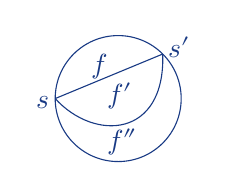
\begin{tikzpicture}[draw=blue,text=blue]\draw (0,0) circle (0.8); \draw (-0.8,0)--(0.5657,0.5657); \draw (-0.8,0) .. controls (-0.3,-0.55) and (0.6,-0.5) .. (0.5657,0.5657); \node at (-0.25,0.4) {$f$}; \node at (0.03,0.03) {$f'$}; \node at (0.05,-0.55) {$f''$}; \node at (-0.95,-0.05) {$s$}; \node at (0.78,0.65) {$s'$};\end{tikzpicture}} $f \cap f'' = \{s,s'\} = S_0$}
ness" condition is now expressed by demanding that the set of indices
I can be totally ordered, \var{\inserted[typed]{i.e. numbered}}{i.e. numbered}{typed insertion}{ps_134-2_027-v0011} in such a way that we get X by succesively
"attaching" \unsure{Dells|cells} $D_{n(i)}$ to the space already constructed\var{\xout{\unsure{,}}}{}{typewriter deletion}{ps_134-2_027-v0012} X(i-1), by a
map from \var{\deleted{a}}{}{deletion}{ps_134-2_027-v0013}\var{\inserted{a sub-}}{\hand{a sub-}}{insertion}{ps_134-2_027-v0014} cell \var{\xout{$D_i$}}{}{typewriter deletion}{ps_134-2_027-v0015}\var{\inserted{of $D_{n(i)}$}}{\hand{of $D_{n(i)}$}}{insertion}{ps_134-2_027-v0016}, $S_j^{\hand{\varepsilon}} \hand{\to} X(i-1)$ \quad $(\hand{\varepsilon\in\{}\pm 1\hand{\}})$ , this map of course
inducing an isomorphism,  more precisely \uline{the} standard isomorphism,\var{\inserted{$\varphi^{\unsure{\varepsilon'}}_{n(i')}$}}{\hand{$\varphi^{\unsure{\varepsilon'}}_{n(i')}$}}{insertion}{ps_134-2_027-v0017}\var{\deleted{of}}{}{deletion}{ps_134-2_027-v0018}
\margin{\textcircled{$\varphi^{\varepsilon'}_{n(i),j}$}}
$S_j^{\hand{\varepsilon}} \hand{\simeq} D_j$ \quad with\var{\inserted{$S^{\varepsilon'}_j$}}{\hand{$S^{\varepsilon'}_j$}}{insertion}{ps_134-2_027-v0019} one of the two corresponding cells $S_j^+$ , $S_j^-$ in some
\margin{\textcircled{$S^{\varepsilon'}_j$}}
$X_{i'} \hand{\simeq} D_{n(i')}$ .  The \var{\xout{xxxxx}}{}{typewriter deletion}{ps_134-2_027-v0020} dual translation of this\hand{,}in terms\hand{\unsure{$\vert$}} of fiber
products in \var{\xout{xxx}}{}{typewriter deletion}{ps_134-2_027-v0021} a category C endowed with objects $F_i$ $(i\in\underline{N})$ and maps
$s_1^i , t_1^i$ between these, is clear:  for a given set of indices I and map
\margin{$P=\prod_{i\in I}F_{n(i)}$}
$i \hand{\mapsto} n(i) : I \hand{\to} \underline{N}$ , we consider a sub\var{\xout{xxx}}{}{typewriter deletion}{ps_134-2_027-v0022}\var{\inserted[typed]{-object}}{-object}{typed insertion}{ps_134-2_027-v0023}\var{\inserted{ of}}{\hand{ of}}{insertion}{ps_134-2_027-v0024} $\var{\inserted[typed]{P=}}{P=}{typed insertion}{ps_134-2_027-v0025}\hand{\prod_{i\in I}}F_{n(i)}$ ,  which can be
described by equality relations between it\var{\over{t}{e}}{\hand{e}}{writing over}{ps_134-2_027-v0026}rated sources and targets
\var{\xout{xxxxxx}}{}{typewriter deletion}{ps_134-2_027-v0027} of various components of $u = (u_i)_{i\in I}$  in P,  the structure of
the set of relations being such that I can\hand{\unsure{,}}be numbered, from 1 to N say,
in such a way that we get in succession \var{\deleted{N}}{}{deletion}{ps_134-2_027-v0028}\var{\inserted{$N-1$}}{\hand{$N-1$}}{insertion}{ps_134-2_027-v0029} relations on the N components
$u_i$ respectively,\var{\inserted{$(2\leq i \leq N)$}}{\hand{$(2\leq i \leq N)$}}{insertion}{ps_134-2_027-v0030} every relation being of the type $f(u_i) = g(u_{i'})$ , with
f and g being iterated source or target maps, and $i'<i$ . \hand{(Whether}
\hand{source or target depending in obvious way on the two signs $\varepsilon,\varepsilon'$.)}

\mspage{\hand{27}}

%% END SOURCE ps_134-2_027
\ifnum\EditionMode=1
\psapparatusstart
\psentry{ps_134-2_027-v0001}{1}{deletion}{\deleted{\illegible{1}}}{}{The author cancels this material by hand; it leaves the corrected running text.}
\psentry{ps_134-2_027-v0002}{2}{insertion}{\inserted{(rather, finite $\varinjlim$'s)}}{\hand{(rather, finite $\varinjlim$'s)}}{The handwritten insertion is incorporated at its indicated position; insertion brackets leave the running text.}
\psentry{ps_134-2_027-v0003}{3}{typewriter deletion}{\xout{\unsure{s}}}{}{The typewriter strikes out this material; it leaves the corrected running text.}
\psentry{ps_134-2_027-v0004}{4}{deletion}{\deleted{cell}}{}{The author cancels this material by hand; it leaves the corrected running text.}
\psentry{ps_134-2_027-v0005}{5}{insertion}{\inserted{cells}}{\hand{cells}}{The handwritten insertion is incorporated at its indicated position; insertion brackets leave the running text.}
\psentry{ps_134-2_027-v0006}{6}{typewriter deletion}{\xout{\unsure{s}}}{}{The typewriter strikes out this material; it leaves the corrected running text.}
\psentry{ps_134-2_027-v0007}{7}{deletion}{\deleted{\illegible{3}}}{}{The author cancels this material by hand; it leaves the corrected running text.}
\psentry{ps_134-2_027-v0008}{8}{insertion}{\inserted{(12)}}{\hand{(12)}}{The handwritten insertion is incorporated at its indicated position; insertion brackets leave the running text.}
\psentry{ps_134-2_027-v0009}{9}{deletion}{\deleted{\illegible{2}}}{}{The author cancels this material by hand; it leaves the corrected running text.}
\psentry{ps_134-2_027-v0010}{10}{writing over}{\over{t}{d}}{\hand{d}}{The superposed handwritten reading replaces the underlying reading.}
\psentry{ps_134-2_027-v0011}{11}{typed insertion}{\inserted[typed]{i.e. numbered}}{i.e. numbered}{The typed insertion is incorporated at its indicated position; insertion brackets leave the running text.}
\psentry{ps_134-2_027-v0012}{12}{typewriter deletion}{\xout{\unsure{,}}}{}{The typewriter strikes out this material; it leaves the corrected running text.}
\psentry{ps_134-2_027-v0013}{13}{deletion}{\deleted{a}}{}{The author cancels this material by hand; it leaves the corrected running text.}
\psentry{ps_134-2_027-v0014}{14}{insertion}{\inserted{a sub-}}{\hand{a sub-}}{The handwritten insertion is incorporated at its indicated position; insertion brackets leave the running text.}
\psentry{ps_134-2_027-v0015}{15}{typewriter deletion}{\xout{$D_i$}}{}{The typewriter strikes out this material; it leaves the corrected running text.}
\psentry{ps_134-2_027-v0016}{16}{insertion}{\inserted{of $D_{n(i)}$}}{\hand{of $D_{n(i)}$}}{The handwritten insertion is incorporated at its indicated position; insertion brackets leave the running text.}
\psentry{ps_134-2_027-v0017}{17}{insertion}{\inserted{$\varphi^{\unsure{\varepsilon'}}_{n(i')}$}}{\hand{$\varphi^{\unsure{\varepsilon'}}_{n(i')}$}}{The handwritten insertion is incorporated at its indicated position; insertion brackets leave the running text.}
\psentry{ps_134-2_027-v0018}{18}{deletion}{\deleted{of}}{}{The author cancels this material by hand; it leaves the corrected running text.}
\psentry{ps_134-2_027-v0019}{19}{insertion}{\inserted{$S^{\varepsilon'}_j$}}{\hand{$S^{\varepsilon'}_j$}}{The handwritten insertion is incorporated at its indicated position; insertion brackets leave the running text.}
\psentry{ps_134-2_027-v0020}{20}{typewriter deletion}{\xout{xxxxx}}{}{The typewriter strikes out this material; it leaves the corrected running text.}
\psentry{ps_134-2_027-v0021}{21}{typewriter deletion}{\xout{xxx}}{}{The typewriter strikes out this material; it leaves the corrected running text.}
\psentry{ps_134-2_027-v0022}{22}{typewriter deletion}{\xout{xxx}}{}{The typewriter strikes out this material; it leaves the corrected running text.}
\psentry{ps_134-2_027-v0023}{23}{typed insertion}{\inserted[typed]{-object}}{-object}{The typed insertion is incorporated at its indicated position; insertion brackets leave the running text.}
\psentry{ps_134-2_027-v0024}{24}{insertion}{\inserted{ of}}{\hand{ of}}{The handwritten insertion is incorporated at its indicated position; insertion brackets leave the running text.}
\psentry{ps_134-2_027-v0025}{25}{typed insertion}{$\inserted[typed]{P=}$}{$P=$}{The typed insertion is incorporated at its indicated position; insertion brackets leave the running text.}
\psentry{ps_134-2_027-v0026}{26}{writing over}{\over{t}{e}}{\hand{e}}{The superposed handwritten reading replaces the underlying reading.}
\psentry{ps_134-2_027-v0027}{27}{typewriter deletion}{\xout{xxxxxx}}{}{The typewriter strikes out this material; it leaves the corrected running text.}
\psentry{ps_134-2_027-v0028}{28}{deletion}{\deleted{N}}{}{The author cancels this material by hand; it leaves the corrected running text.}
\psentry{ps_134-2_027-v0029}{29}{insertion}{\inserted{$N-1$}}{\hand{$N-1$}}{The handwritten insertion is incorporated at its indicated position; insertion brackets leave the running text.}
\psentry{ps_134-2_027-v0030}{30}{insertion}{\inserted{$(2\leq i \leq N)$}}{\hand{$(2\leq i \leq N)$}}{The handwritten insertion is incorporated at its indicated position; insertion brackets leave the running text.}
\psapparatusend
\fi

\end{document}
